%%%%%%%%%%%%%%%%%%%%%%%%%%%%%%%%%%%%%%%%%%%%%%%%%%%%%%%%%%%%%%%%%%%%%%%%%%%%%%%%
%
% Template license:
% CC BY-NC-SA 3.0 (http://creativecommons.org/licenses/by-nc-sa/3.0/)
%
%%%%%%%%%%%%%%%%%%%%%%%%%%%%%%%%%%%%%%%%%%%%%%%%%%%%%%%%%%%%%%%%%%%%%%%%%%%%%%%%
%----------------------------------------------------------------------------------------
%	PACKAGES AND OTHER DOCUMENT CONFIGURATIONS
%----------------------------------------------------------------------------------------

\documentclass[
11pt, % The default document font size, options: 10pt, 11pt, 12pt
%oneside, % Two side (alternating margins) for binding by default, uncomment to switch to one side
%chapterinoneline,% Have the chapter title next to the number in one single line
spanish,
singlespacing, % Single line spacing, alternatives: onehalfspacing or doublespacing
%draft, % Uncomment to enable draft mode (no pictures, no links, overfull hboxes indicated)
%nolistspacing, % If the document is onehalfspacing or doublespacing, uncomment this to set spacing in lists to single
%liststotoc, % Uncomment to add the list of figures/tables/etc to the table of contents
%toctotoc, % Uncomment to add the main table of contents to the table of contents
parskip, % Uncomment to add space between paragraphs
codirector, % Uncomment to add a codirector to the title page
headsepline, % Uncomment to get a line under the header
]{MastersDoctoralThesis} % The class file specifying the document structure



%----------------------------------------------------------------------------------------
%	INFORMACIÓN DE LA MEMORIA
%----------------------------------------------------------------------------------------

\thesistitle{Emulador de la placa EDU-CIAA} % El títulos de la memoria, se usa en la carátula y se puede usar el cualquier lugar del documento con el comando \ttitle

% Nombre del posgrado, se usa en la carátula y se puede usar el cualquier lugar del documento con el comando \degreename
%\posgrado{Carrera de Especialización en Sistemas Embebidos} 
%\posgrado{Carrera de Especialización en Internet de las Cosas} 
%\posgrado{Carrera de Especialización en Intelegencia Artificial}
\posgrado{Maestría en Sistemas Embebidos} 
%\posgrado{Maestría en Internet de las cosas}

\author{Esp. Ing. Jenny Chavez} % Tu nombre, se usa en la carátula y se puede usar el cualquier lugar del documento con el comando \authorname

\director{Dr. Ing. Pablo Gomez (FIUBA)} % El nombre del director, se usa en la carátula y se puede usar el cualquier lugar del documento con el comando \dirname
\codirector{Mg. Ing. Eric Pernía (UNQ, FIUBA)} % El nombre del codirector si lo hubiera, se usa en la carátula y se puede usar el cualquier lugar del documento con el comando \codirname.  Para activar este campo se debe descomentar la opción "codirector" en el comando \documentclass, línea 23.

\juradoUNO{Mg. Ing. Gonzalo Sánchez (FF.AA, FIUBA)} % Nombre y pertenencia del un jurado se usa en la carátula y se puede usar el cualquier lugar del documento con el comando \jur1name
\juradoDOS{Mg. Ing. Iván Andrés León Vásquez (INVAP)} % Nombre y pertenencia del un jurado se usa en la carátula y se puede usar el cualquier lugar del documento con el comando \jur2name
\juradoTRES{Ing. Juan Manuel Cruz (FIUBA/UTN)} % Nombre y pertenencia del un jurado se usa en la carátula y se puede usar el cualquier lugar del documento con el comando \jur3name

\ciudad{Ciudad Autónoma de Buenos Aires}
%\ciudad{ciudad de Mendoza}

\fechaINICIO{agosto de 2019}
\fechaFINAL{agosto de 2023}


\keywords{Sistemas embebidos, FIUBA} % Keywords for your thesis, print it elsewhere with \keywordnames


\begin{document}


\frontmatter % Use roman page numbering style (i, ii, iii, iv...) for the pre-content pages

\pagestyle{plain} % Default to the plain heading style until the thesis style is called for the body content


%----------------------------------------------------------------------------------------
%	RESUMEN - ABSTRACT 
%----------------------------------------------------------------------------------------

\begin{abstract}
\addchaptertocentry{\abstractname} % Add the abstract to the table of contents
%
%The Thesis Abstract is written here (and usually kept to just this page). The page is kept centered vertically so can expand into the blank space above the title too\ldots
\centering

La presente memoria describe el diseño e implementación de una plataforma web que emula la placa EDU-CIAA-NXP y permite desarrollar en lenguaje C sin la necesidad de tener la placa real. La interfaz de la plataforma permite escribir, probar y verificar aplicaciones rápidamente de una manera amigable y nace como una herramienta de aprendizaje para ser parte del Proyecto CIAA.

Para la realización de este trabajo fueron fundamentales los conocimientos relacionados al diseño de software, gestión de la tecnología e innovación, implementación de manejadores de dispositivos, sistema operativo de tiempo real, desarrollo de aplicaciones sobre sistemas operativos de propósito general y testing de sistemas embebidos. 

\end{abstract}

%----------------------------------------------------------------------------------------
%	CONTENIDO DE LA MEMORIA  - AGRADECIMIENTOS
%----------------------------------------------------------------------------------------

\begin{acknowledgements}
%\addchaptertocentry{\acknowledgementname} % Descomentando esta línea se puede agregar los agradecimientos al índice
\vspace{1.5cm}

Al Director de este trabajo Dr. Ing. Pablo Martín Gomez
y al Codirector Mg. Ing. Eric Pernia.

\end{acknowledgements}

%----------------------------------------------------------------------------------------
%	LISTA DE CONTENIDOS/FIGURAS/TABLAS
%----------------------------------------------------------------------------------------

\tableofcontents % Prints the main table of contents

\listoffigures % Prints the list of figures

\listoftables % Prints the list of tables


%----------------------------------------------------------------------------------------
%	CONTENIDO DE LA MEMORIA  - DEDICATORIA
%----------------------------------------------------------------------------------------

\dedicatory{\textbf{Dedicado a mi familia}}  % escribir acá si se desea una dedicatoria

%----------------------------------------------------------------------------------------
%	CONTENIDO DE LA MEMORIA  - CAPÍTULOS
%----------------------------------------------------------------------------------------

\mainmatter % Begin numeric (1,2,3...) page numbering

\pagestyle{thesis} % Return the page headers back to the "thesis" style

% Incluir los capítulos como archivos separados desde la carpeta Chapters

% Chapter 1
%\label{Chapter1} % For referencing the chapter elsewhere, use \ref{Chapter1} 

%----------------------------------------------------------------------------------------

% Define some commands to keep the formatting separated from the content 
\newcommand{\keyword}[1]{\textbf{#1}}
\newcommand{\tabhead}[1]{\textbf{#1}}
\newcommand{\code}[1]{\texttt{#1}}
\newcommand{\file}[1]{\texttt{\bfseries#1}}
\newcommand{\option}[1]{\texttt{\itshape#1}}
\newcommand{\grados}{$^{\circ}$}

%----------------------------------------------------------------------------------------

\chapter{Introducción general} % Main chapter title
\label{IntroGeneral}

%----------------------------------------------------------------------------------------
% Resumen de capitulo
%----------------------------------------------------------------------------------------

En este capítulo se exponen las problemáticas encontradas con el hardware en el estudio de los Sistemas Embebidos, que motiva la realización de un emulador para la placa EDU-CIAA-NXP \citep{EDU-CIAA-NXP}. Presentando los objetivos, el alcance, los requerimientos y la metodología de trabajo utilizada para llevar a cabo este proyecto.

%----------------------------------------------------------------------------------------
\section{Motivación}
%----------------------------------------------------------------------------------------

Los emuladores son desarrollos de software que modelan el funcionamiento del hardware real, de manera que permiten ejecutar programas dentro de un ambiente que imita su comportamiento \citep{sanchezqemu}. De esta forma un usuario puede simular su código antes de instalarlo en el dispositivo físico.

Para colaborar con la enseñanza de la programación de Sistemas Embebidos, se propuso, como parte del Proyecto CIAA \citep{CIAA}, realizar una plataforma de software que emule el funcionamiento de la placa EDU-CIAA-NXP, así como los periféricos y placas que se pueden conectar a ella.

Esto se debe a que para el desarrollo de aplicaciones en sistemas embebidos es necesario tener de antemano la placa de desarrollo y los componentes de hardware externos a conectar a la placa, para poder probar los programas realizados. Además, muchas veces un usuario sin experiencia, no cuenta con los dispositivos para comenzar, se equivoca en la selección de los mismos, o en las conexiones eléctricas, provocando daños irreparables en el hardware. 

De esta manera, mediante el uso de un emulador se evita todos estos inconvenientes y permite al usuario probar sus programas rápidamente, enfocándose en el desarrollo de aplicaciones y ejecutando sus pruebas en un sistema virtual, dejando para más adelante la implementación en el hardware real.

Un aspecto importante a destacar es el alto costo del hardware y la variedad de dispositivos necesarios. Entonces, contar con un emulador habilita a personas con bajos recursos aprender a programar Sistemas Embebidos utilizando hardware virtual, que se comporta como el hardware real, permitiendo probar diferentes tecnologías.

Para disponibilizar esta herramienta lo más posible, se decidió construir una plataforma de desarrollo con interfaz gráfica dentro de un entorno web, accesible a través de un navegador. De esta manera, se obtiene una herramienta que esté disponible de forma \textit{on line}, para que pueda usarse de forma gratuita, tanto en Computadoras, Tablets o Smartphones, como puede observarse en al figura \ref{fig:EsquemaEmulador}.

\begin{figure}[ht]
	\centering
	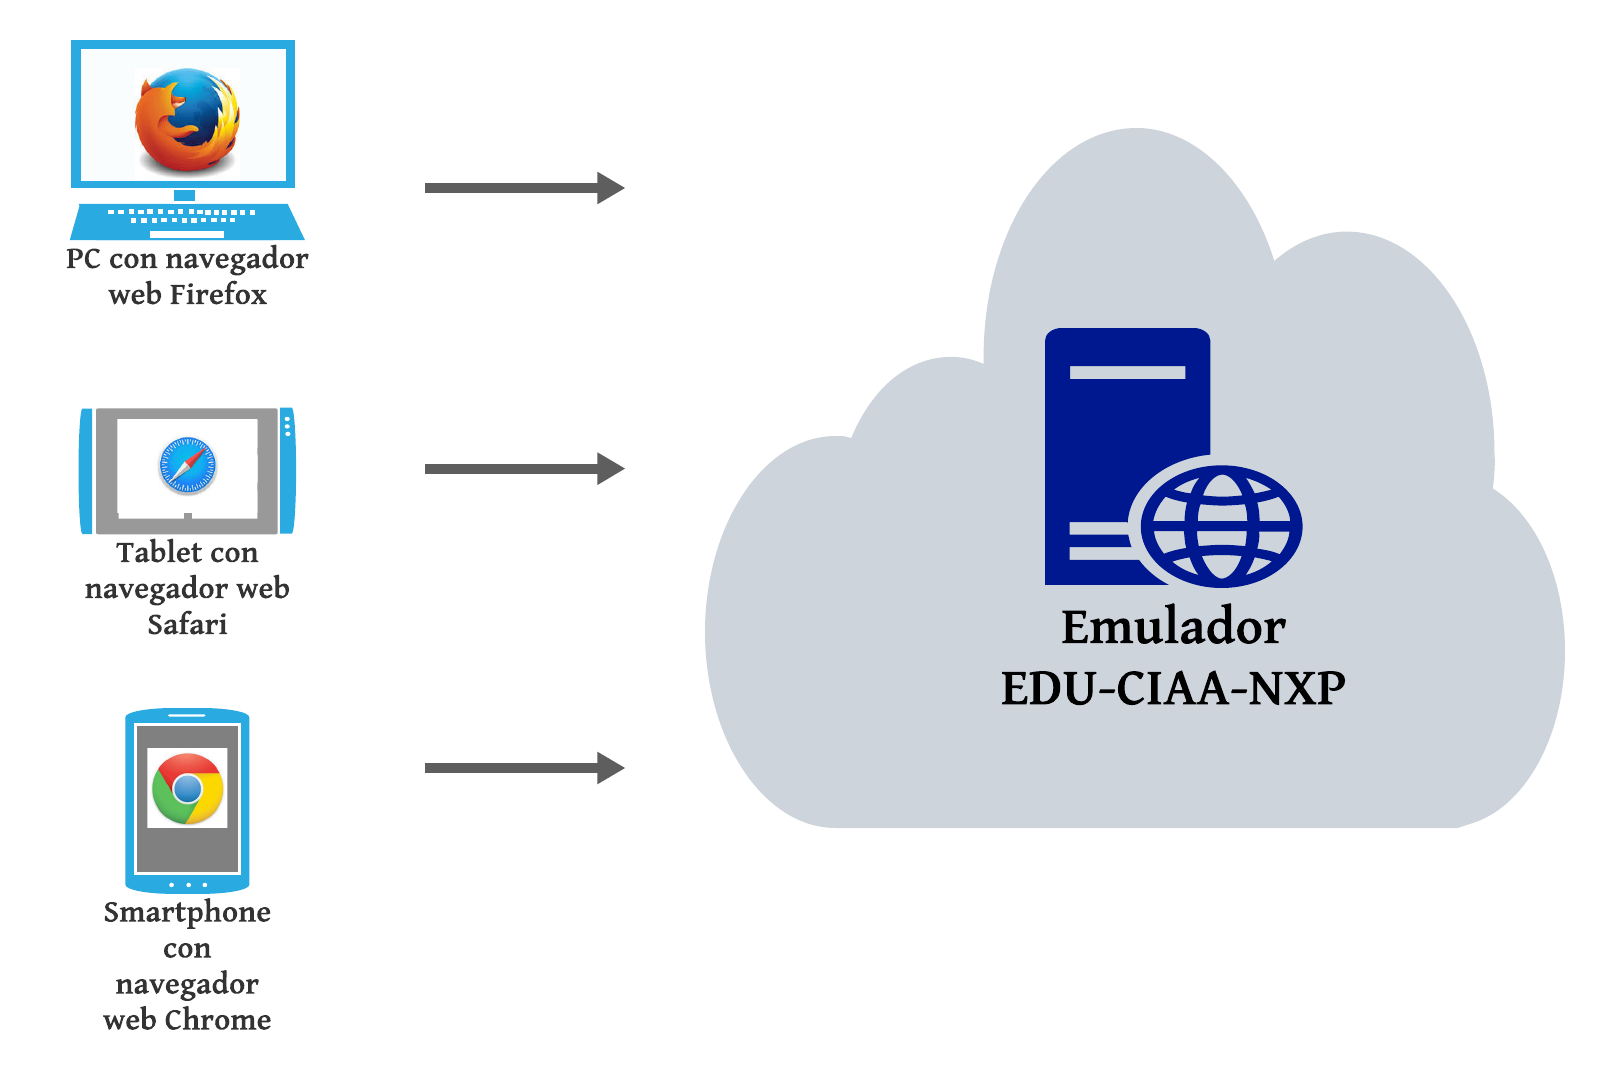
\includegraphics[scale=.55]{./Figures/EsquemaEmuladorCh1.png}
	\caption{Esquema Emulador EDU-CIAA-NXP.}
	\label{fig:EsquemaEmulador}
\end{figure}

En otras palabras, con esta herramienta de emulación, una persona que recién comienza tendrá la experiencia de relacionarse con un sistema embebido solamente conectandose mediante internet a la aplicación web en su ordenador, liberando así el camino a los estudiantes novatos de hacer la interacción con el hardware.

La autora del presente trabajo ha colaborado previamente en el Proyecto CIAA, mediante el desarrollo del software CIAA-BOT Debug como Trabajo Final de la Carrera en Especialización en Sistemas Embebidos de la FI-UBA \citep{TrabajoFinalCESE}, que permite depurar programas realizados mediante el lengaje gráfico CIAA-BOT.

%----------------------------------------------------------------------------------------
\section{Objetivos}
%----------------------------------------------------------------------------------------

Dados los antecedentes explicados, el objetivo de este trabajo es desarrollar una herramienta educativa que brinda un entorno virtual para la placa EDU-CIAA-NXP, permitiendo al usuario seleccionar y conectar con la EDU-CIAA-NXP diferentes tipos de dispositivos virtuales e interactuar con los mismos. Este desarrollo permite al usuario cargar, ejecutar, editar y corregir sus programas escritos en lenguaje C, pudiendo monitorizar gráficamente en la pantalla del ordenador la placa EDU-CIAA-NXP y muchos de los dispositivos de entrada y salida más comunes, todo de manera virtual, sin necesidad de disponer de ningún dispositivo de hardware.

%----------------------------------------------------------------------------------------
\section{Alcance}
%----------------------------------------------------------------------------------------

En el presente trabajo se realizó una primera versión de la herramienta para ser usada con la placa EDU-CIAA-NXP. En particular, se incluyen los siguientes aspectos:

\begin{enumerate}
	\item Desarrollo de aplicación para emular el hardware en PC.
	\item Realización de programas de ejemplo para ser usados dentro de la aplicación.
	\item Documentación de referencia.
\end{enumerate}

El presente proyecto no incluye el desarrollo de la aplicación para emular otras placas que no sea EDU-CIAA-NXP.

%----------------------------------------------------------------------------------------
\section{Requerimientos}
\label{sec:Requerimientos}
%----------------------------------------------------------------------------------------

Se han identificado los siguientes requerimientos:

\begin{enumerate}
    \item Investigación y definición de la arquitectura del software.
        \begin{enumerate}
            \item Investigar sobre las plataformas de emulación de hardware existentes.
            \item Investigar la arquitectura y funcionamiento de las bibliotecas y ejemplos para la EDU-CIAA-NXP, disponibles en firmware v3 \citep{firmwareV3}.
        \end{enumerate}
    \item Desarrollo del Emulador.
        \begin{enumerate}
            \item Realizar la aplicación para emular el hardware.
            \item Integrar las bibliotecas de lenguaje C de la placa EDU-CIAA-NXP portándolas a la paltaforma virtual.
            \item Respetar el estilo de código de las bibliotecas.
            \item Portar ejemplos de utilización de las bibliotecas.
            \item Desarrollar nuevos ejemplos.
        \end{enumerate}
    \item Documentación del proyecto.
        \begin{enumerate}
            \item Elaborar la documentación de la plataforma.
            \item Confeccionar un manual de usuario.
        \end{enumerate}
\end{enumerate}

%----------------------------------------------------------------------------------------
\section{Metodología de trabajo}
%----------------------------------------------------------------------------------------

Para el desarrollo de este trabajo se eligió utilizar las siguientes prácticas:

\begin{itemize}
    \item Utilizar software libre para el desarrollo del proyecto. Reutilizar todo el software y ejemplos disponibles, tanto del Proyecto CIAA como de terceros.
    \item Utilizar un Sistema de Control de Versiones de código fuente distribuído \citep{ControlVersionesGIT}.
    \item Desarrollar \textit{tests} unitarios y de integración.
    \item Automatizar los \textit{tests} y \textit{deployments} mediante Integración Continua \citep{IntegraciónContinuaGIT}.
\end{itemize}

\chapter{Introducción específica} % Main chapter title
\label{Chapter2}

%----------------------------------------------------------------------------------------
% Resumen de capitulo
%----------------------------------------------------------------------------------------

En el presente capítulo se describe el estado actual de algunas soluciones implementadas, y se elige una plataforma existente, que cumple con los requerimientos del trabajo como base. También, se presenta el estudio del código fuente de \textit{Arm Mbed OS Simulator}. 

%----------------------------------------------------------------------------------------
\section{Estado del arte}
\label{sec:Estado del arte}
%----------------------------------------------------------------------------------------

Hoy en día no existe una herramienta de emulación para la placa EDU-CIAA-NXP. Sin embargo, existe la plataforma de código abierto ViHard \citep{ViHard} que emula dispositivos de hardware en la PC, pero con la placa ECU-CIAA-NXP real conectada a la PC a través del puerto USB. En la figura \ref{fig:ViHard} se muestra el esquema de la plataforma ViHard.

\begin{figure}[ht]
	\centering
	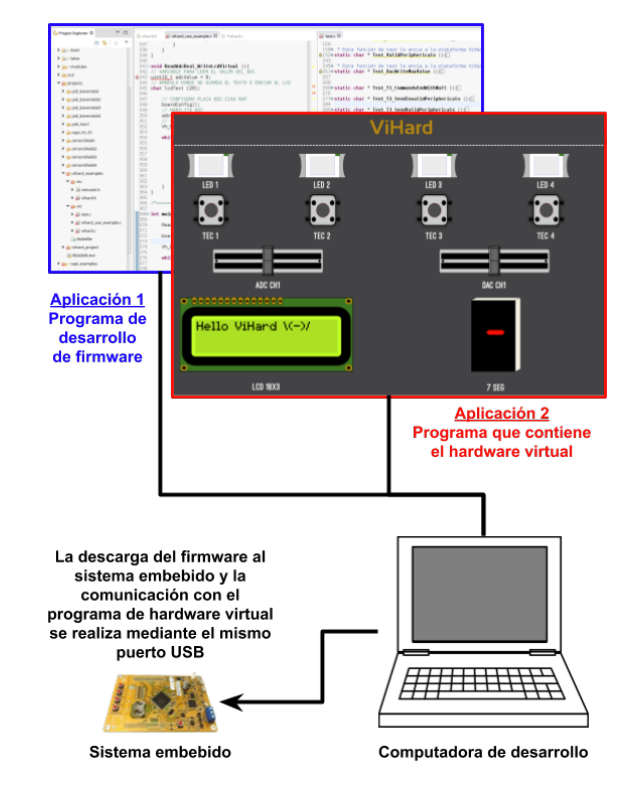
\includegraphics[scale=.40]{./Figures/ViHard.png}
	\caption{Esquema de la plataforma ViHard.\protect\footnotemark}
	\label{fig:ViHard}
\end{figure}

La plataforma se compone de un programa de PC con los perifericos virtuales de hardware y una biblioteca de firmware para la EDU-CIAA-NXP, que controla y gestiona el funcionamiento del hardware virtual. Ambos programas se comunican con el sistema embebido mediante UART, a través de un puerto USB.

El programa de hardware virtual es una aplicacion de escritorio multiplataforma desarrollada utilizando el framework Electron \citep{Electron}. Por otro lado, la biblioteca embebida fue desarrollada en lenguaje C. 

Por lo tanto, el usuario necesita ejecutar en su PC el programa de periféricos virtuales y contar con la biblioteca en el sistema embebido que controla el hardware virtual. A partir de ahí, procedería al desarrollo de su propio programa, que deberá compilar y descargar a la EDU-CIAA-NXP, y posteriormente realizar las pruebas correspondientes.

Por otro lado, se encontraron muchas plataformas educativas que simulan microcontroladores, sobre todo para la placa Arduino \citep{Arduino}. Para el análisis, se seleccionaron algunos de los simuladores más populares que implementan funcionalidades relevantes para el presente trabajo, los cuales se describen en las siguientes secciones. 

%------------------------------------
\subsection{UnoArduSim}

UnoArduSim \citep{UnoArduSim} fue desarrollado en la Universidad de Queen \citep{Queensu} por el profesor Stan Simmons. En la figura \ref{fig:UnoArduSim} puede observarse la interfaz del programa.

\begin{figure}[ht]
	\centering
	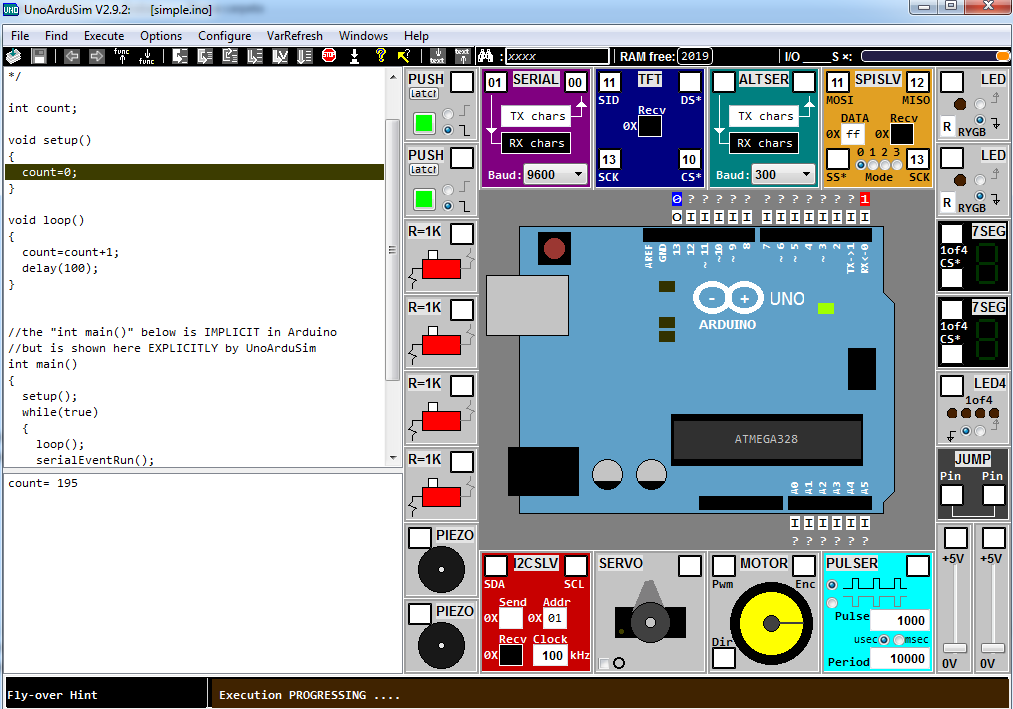
\includegraphics[scale=.33]{./Figures/UnoArduSim.png}
	\caption{Plataforma UnoArduSim.}
	\label{fig:UnoArduSim}
\end{figure}

La herramienta simula en la pantalla de la PC la placa Arduino Uno \citep{ArduinoUno} y muchos de los dispositivos de entrada y salida más usados, asimismo, permite la depuración interactiva de funciones o programas completos. Está diseñada específicamente para ejecutarse en el sistema operativo Windows. Además, el diseño de la interfaz gráfica no promueve la claridad visual, puesto que hay demasiados objetos en la pantalla y los que existen deberían estar mejor distribuidos. 

%------------------------------------
\subsection{Virtronics}

Virtronics \citep{Virtronics} es uno de los simuladores más completos que hay hoy en día para Arduino \citep{Arduino}, ya que permite simular varios modelos y, además, tiene dos versiones disponibles: una versión paga y otra gratuita, pero con funciones limitadas. En la figura \ref{fig:Virtronics} se muestra la plataforma.

\begin{figure}[ht]
	\centering
	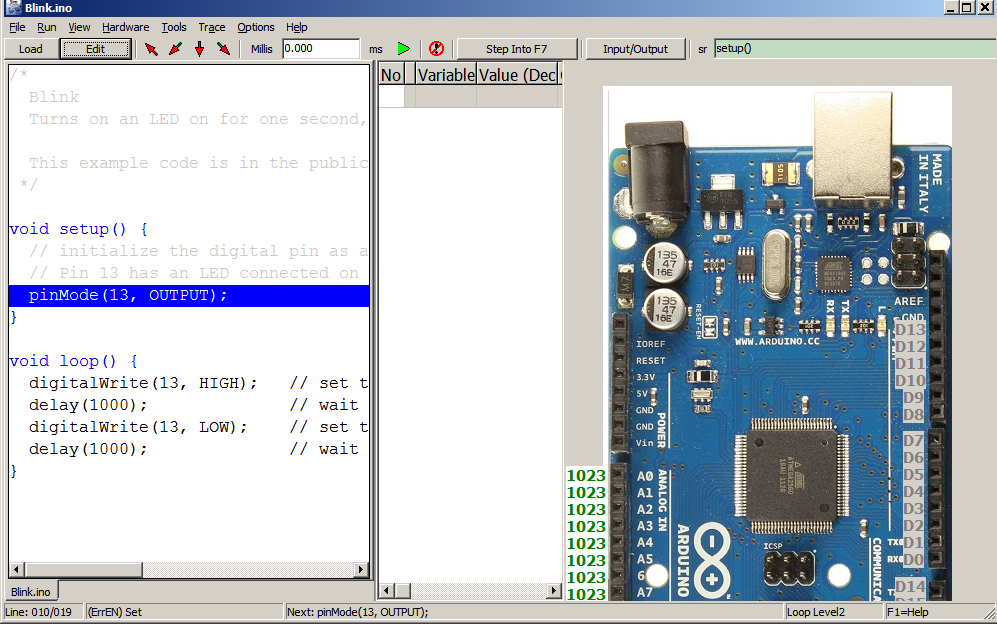
\includegraphics[scale=.35]{./Figures/Virtronics.png}
	\caption{Plataforma Virtronics.}
	\label{fig:Virtronics}
\end{figure}

%------------------------------------
\subsection{Tinkercad}

Tinkercad \citep{Tinkercad} es una plataforma online que permite el acceso desde cualquier navegador web, cuya interfaz de usuario se muestra en la figura \ref{fig:Tinkercad}.

\begin{figure}[ht]
	\centering
	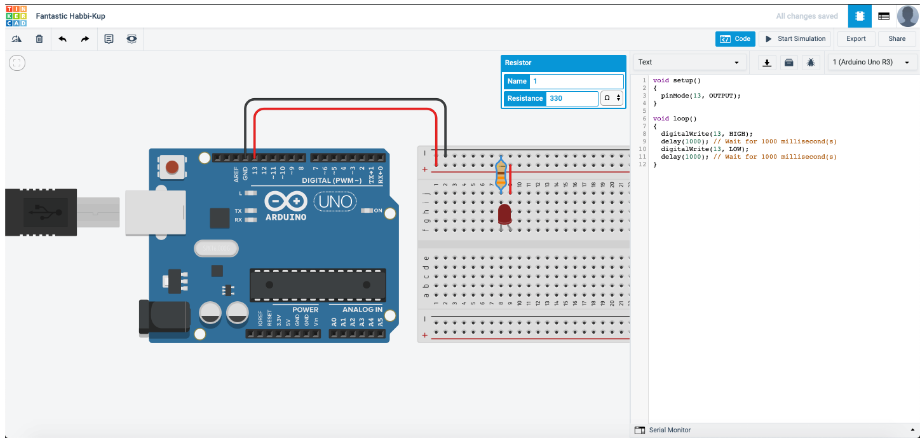
\includegraphics[scale=.40]{./Figures/Tinkercad.png}
	\caption{Plataforma Tinkercad.}
	\label{fig:Tinkercad}
\end{figure}

Fue desarrollado por ingenieros y diseñadores de software de Autodesk \citep{Autodesk} y permite diseños 3D. Adicionalmente, es necesario crear una cuenta  antes de empezar a usar la plataforma, por consiguiente, todos los diseños se guardan en la cuenta creada. 

%------------------------------------
\subsection{\textit{Arm Mbed OS Simulator}}

\textit{Arm Mbed OS Simulator} \citep{ArmMbedSim} fue desarrollado por ingenieros de Arm, encargados de mantener las bibliotecas Mbed OS, \citep{ArmMbed} y es parte de Mbed Labs. La plataforma era accesible \textit{on line} al momento del comienzo de este proyecto, pero actualmente debe ser descargado desde su repositorio \citep{ArmMbedSimRepo} y luego, puede ejecutarse utilizando cualquier navegador web en la red local, o bien, realizar el despliegue en un servidor para que esté disponible \textit{on line}. En la figura \ref{fig:ArmMbed} puede observarse la plataforma online de Mbed Simulator.

\begin{figure}[ht]
	\centering
	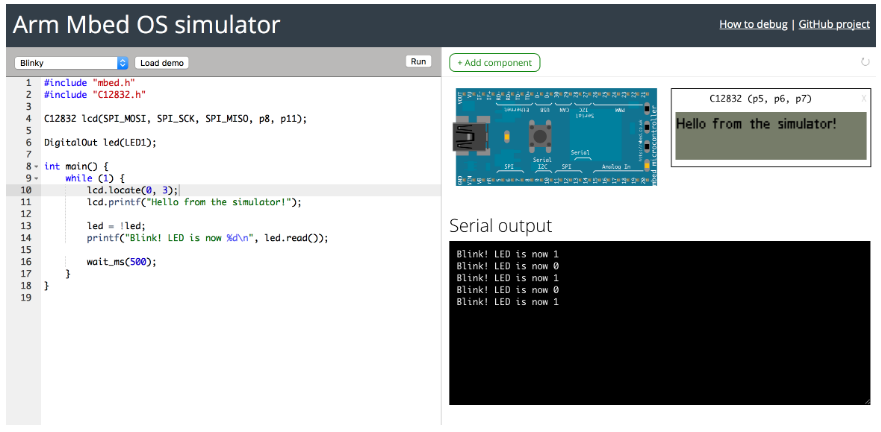
\includegraphics[scale=.44]{./Figures/ArmMbed.png}
	\caption{Plataforma Arm Mbed OS Simulator.}
	\label{fig:ArmMbed}
\end{figure}

El funcionamiento de este emulador es muy simple. Se puede crear un programa desde cero, o bien, se puede elegir un ejemplo de la lista desplegable y cargar el proyecto desde el botón \textquotedbl Load demo\textquotedbl, luego añadir los componentes necesarios para el programa, como por ejemplo, el display que se observa en la figura \ref{fig:ArmMbed}, donde se pide al usuario indicar a qué pines estará conectado. Es importante mencionar que el programa ya incluye la placa con el microcontrolador precargada. Una vez completo el programa y el ensamblado del hardware, se puede compilar y ejecutar en el emulador usando el botón \textquotedbl Run\textquotedbl.

%----------------------------------------------------------------------------------------
\section{Análisis de los emuladores revisados}
\label{sec:Análisis de los emuladores revisados}
%----------------------------------------------------------------------------------------

En la tabla \ref{tab:simuladores} se comparan las características más importantes de estos emuladores. 

\hfill \break
\hfill \break
\hfill \break
\hfill \break
\hfill \break
\hfill \break
\hfill \break
\hfill \break
\hfill \break

\begin{table}[ht]
\centering
\caption[Comparación de características de los emuladores revisados]{Comparación de características de los emuladores revisados}
\begin{tabular}{p{0.24\linewidth} p{0.17\linewidth}  p{0.19\linewidth}  p{0.14\linewidth}  p{0.10\linewidth}}
\toprule
\textbf{Característica} 
& \textbf{UnoArduSim}
& \textbf{Virtronics}
& \textbf{Tinkercad}
& \textbf{Mbed OS}
\\
\midrule
Placa/Plataforma emulada & Arduino Uno & Varios modelos Arduino & Arduino Uno & Arm Mbed OS\\
Gratuito &    Sí & No & Sí & Sí\\
Aplicación & Escritorio & Escritorio & Web & Web\\
Plataforma & Windows & Windows/Linux & Todas & Todas\\
Código abierto & No & No & No & Sí\\
Dispositivos E/S & Sí & Sí & Sí & Sí  \\
Panel de desarrollo & Sí & Sí & Sí & Sí \\
Lenguaje & C & C & C & C/C++\\
Debugging & Sí & Sí & Sí & No\\
Ejemplos & Sí & Sí & Sí & Sí\\
\bottomrule
\hline
\end{tabular}
\label{tab:simuladores}
\end{table}

Cabe destacar, que de las plataformas revisadas \textit{Arm Mbed OS Simulator} es la única de código abierto. Sin embargo, este análisis sirve tembién para revisar, comprender y comparar las ventajas y desventajas de las otras plataformas, y tomar características útiles para el desarrollo del emulador. 

Del análisis anterior, se desprende que \textit{Arm Mbed OS Simulator} presenta las siguientes ventajas significativas:

\begin{itemize}
	\item Código abierto: al tener acceso al código fuente permitió estudiar cómo funciona internamente el proyecto simulador, además, de la libertad de uso y distribución.
	\item Arquitectua de aplicación web. 
    \item Su capacidad para simular dispositivos y componentes.
	\item Comunidad y Soporte: el proyecto tiene una comunidad activa de desarrolladores, que brinda acceso a una amplia base de conocimientos, documentación y soporte. 
	\item Reconocimiento de Marca ARM mbed OS: al basarse en su proyecto simulador, se puede obtener cierto reconocimiento y confianza entre los usuarios.
	\item Reutilización: ofrece un conjunto sólido de funcionalidades y características ya probadas que agilizó el desarrollo y redujo la probabilidad de introducir errores.
	\item Actualizaciones y Mejoras Continuas: el proyecto Mbed Simulator recibe actualizaciones continuas con las últimas tecnologías que permite mantener el emulador para la placa EDU-CIAA-NXP actualizado.	
\end{itemize}

Sim embargo, actualmente, \textit{Arm Mbed OS Simulator} presenta las siguientes limitaciones:

\begin{enumerate}
	\item Dentro de un bucle infinito \texttt{while(1)}, es necesario agregar un retraso \newline(\texttt{delay)}, de lo contrario, el navegador no puede actualizar la interfaz de la plataforma web ni responder a eventos del usuario. Esto significa que el navegador no tiene la oportunidad de realizar otras tareas o responder a eventos mientras el bucle está en ejecución. Como resultado, el navegador se bloquea o congela y puede dejar de responder.
	
	\item En cada iteracion, la ejecución del programa puede variar en términos de tiempo, lo que puede afectar a la precisión en la sincronización de eventos dentro de la aplicación.

	\item En \textit{Arm Mbed OS Simulator}, no hay restricciones significativas en cuanto a la cantidad de memoria que se puede asignar al stack o al heap  de un programa, lo cual difiere del hardware físico, donde sí existen limitaciones de memoria.
	
	\item Dentro del entorno web, las interrupciones no se manejan de la misma manera que en un sistema embebido real, debido a que no implementa el manejo de prioridades, por lo cual no afectan la ejecución del programa principal.
	
	\item Sin RTOS. No tiene la capacidad de ejecutar múltiples hilos de manera concurrente como lo haría un RTOS. Todo el código se ejecuta en un solo hilo. Se puede utilizar la biblioteca mbed-events para manejar ciertos aspectos de concurrencia, usando eventos y temporizadores.
	
	\item Emulación a nivel API de Mbed OS. No permite programar a bajo nivel, utilizando registros de core para la arquitectura ARM o periféricos.
	
	\item Sin capacidad de debug paso a paso. Se realiza el programa, se compila y ejecuta en el hardware virtual pero no permite la depuración de código.
\end{enumerate}

Dadas todas estas consideraciones y una vez confirmada su compatibilidad para los propósitos del presente trabajo, se decide basar el emulador de la EDU-CIAA-NXP en portar el proyecto \textit{Arm Mbed OS Simulator}, para la EDU-CIAA-NXP y sus bibliotecas.

%----------------------------------------------------------------------------------------
\section{Análisis del código fuente de \textit{Arm Mbed OS Simulator}}
%----------------------------------------------------------------------------------------

Se procedió a analizar en detalle el código fuente de \textit{Arm Mbed OS Simulator} para adquirir una compresión de su arquitectura, del funcionamiento del \textit{Sistema Operativo Mbed}, de los periféricos simulados y sus las interacciones, así como de las configuraciones necesarias para la plataforma web.

%------------------------------
\subsection{Análisis de las tecnologías utilizadas}

\textit{Arm Mbed OS Simulator} es una aplicación web. Este tipo de aplicaciones son provistas por un servidor web y pueden ser accedidas por los usuarios que se conecten a través de internet desde cualquier lugar mediante un navegador web \citep{NavegadorWeb}. Además, presentan la arquitectura cliente/servidor (que se muestra en la figura \ref{fig:ClienteServidor}) en donde un cliente o navegador web realiza peticiones al servidor y en consecuencia el servidor envía la respuesta de regreso.

\begin{figure}[ht]
	\centering
	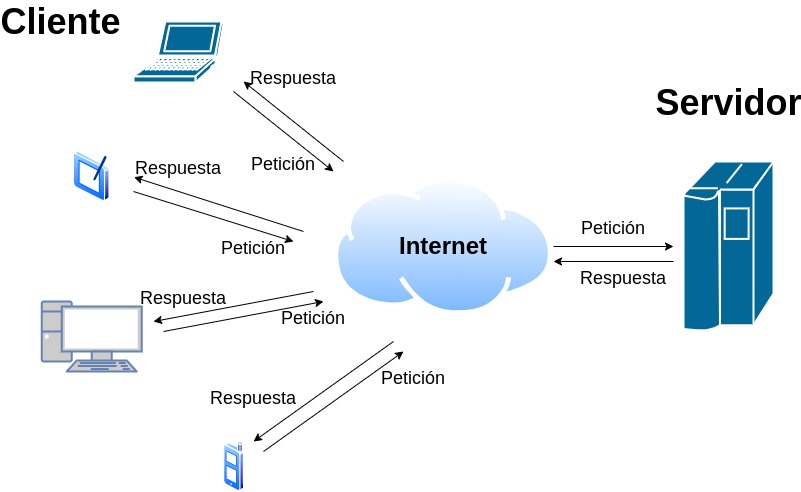
\includegraphics[scale=.48]{./Figures/EsquemaCliente_Servidor.jpg}
	\caption{Esquema modelo cliente/servidor.}
	\label{fig:ClienteServidor}
\end{figure}

\hfill \break
\hfill \break
\hfill \break

Las razones por las que se optó por la tecnologia web se debe a las potenciales ventajas que presentan, de las cuales las más importantes son:

\begin{itemize}
	\item No es necesario instalar nada en la computadora del usuario.
	\item No consumen los recursos del ordenador.
	\item No se encuentra limitado a un lugar físico específico para acceder y utilizar las capacidades de emulación.
	\item No obliga al usuario usar un determinado sistema operativo, ya que se puede ejecutar en todos los dispositivos con acceso a un navegador web y una conexión a internet.
\end{itemize}

En el desarrollo web, el \textit{frontend} es la parte del software que interactúa con el usuario y el \textit{backend} es la parte lógica que se encarga de tomar los datos, procesarlos y devolverlos al \textit{frontend}. En la figura \ref{fig:frontBackMbed} se muestra un esquema con las tecnologías web usadas en el presente trabajo.

\hfill \break
\hfill \break
\hfill \break
\hfill \break
\hfill \break
\hfill \break
\hfill \break
\hfill \break
\hfill \break
\hfill \break
\hfill \break
\hfill \break

\begin{figure}[ht]
	\centering
	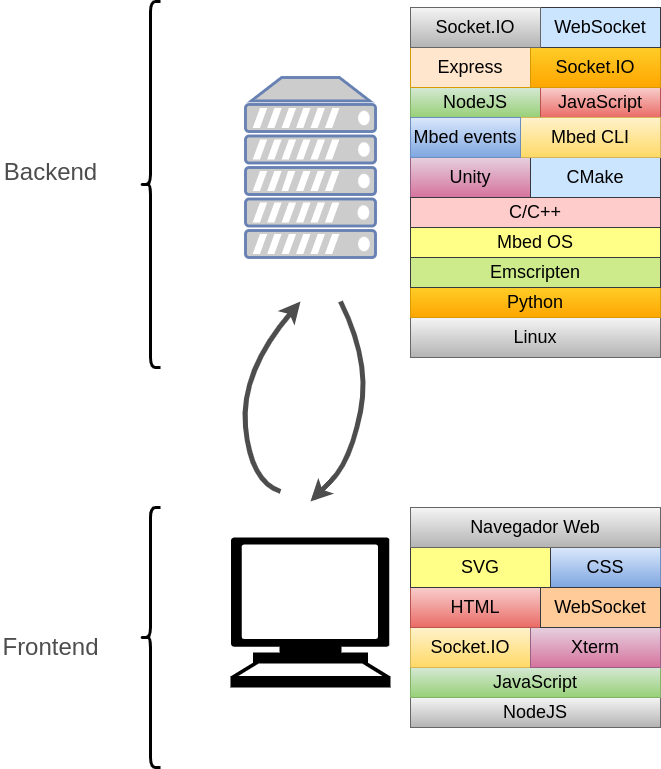
\includegraphics[scale=.47]{./Figures/FrontendBackendMbed.png}
	\caption{Esquema de las tecnologías utlilizadas en \textit{Arm Mbed OS Simulator}.}
	\label{fig:frontBackMbed}
\end{figure}

En las siguientes secciones se describen las tecnologías que forman parte del \textit{frontend} y \textit{backend} del emulador.

%-------------------------
\subsection{Frontend}
\label{subsec:Frontend}

Se describen brevemente las principales tecnologías utilizadas:

\begin{itemize}
	\item JavaScript \citep{JavaScript}: es un lenguaje de programación que se ejecuta del lado del cliente en el navegador, o bien del lado del servidor mediante motores como NodeJS \citep{NodeJS}. En el caso del lado del cliente, permite crear páginas web dinámicas y también responder a eventos causados por el propio usuario tales como modificaciones del DOM, de la sigla en inglés  \textit{Document Object Model} \citep{DOM}. Por consiguiente, el desarrollo con JavaScript en el frontend permitió cargar y ejecutar los archivos resultantes generados por el compilador en el navegador. Asimismo, es el responsable de configurar el entorno necesario para ejecutar el emulador web y proporcionar la interfaz de usuario para la interacción. Además, en el backend fue útil para gestionar la comunicación y la interacción entre los diferentes componentes a través de solicitudes HTTP, permitiendo la transferencia de datos y el flujo de información dentro de la plataforma web.

	\item NodeJS \citep{NodeJS}: es un entorno de ejecución de JavaScript cuyo propósito es el desarrollo de aplicaciones web y servicios del lado del servidor. También, proporciona una arquitectura orientada a eventos y no bloqueante. 
De manera que, en el contexto del frontend, se utilizó como parte del flujo de trabajo de desarrollo, incluyendo la gestión de dependencias, automatización de tareas de compilación, pruebas y despliegue. Mientras tanto, en el backend, se utilizó para desarrollar las rutas, controladores y manejar la lógica de la aplicación en respuesta a las solicitudes entrantes y el envío de respuestas.

	\item HTML \citep{HTML}: de la sigla en inglés \textit{Lenguaje de Marcas de Hipertexto, del inglés HyperText Markup Language}, es el lenguaje de marcas que sirve para etiquetar contenido y visualizarlos en el navegador web.
	Este lenguaje es sencillo de aprender y es fácil de interpre­tar tanto por humanos como por máquinas.  En el desarrollo, se utilizó para crear los elementos visuales de la interfaz de usuario, como los botones, lista desplegable, pantallas de visualización, y otros componentes necesarios para interactuar con el emulador web.

	\item CSS \citep{CSS}: de la sigla en inglés \textit{Cascading Style Sheets},
	es un lenguaje de diseño gráfico que permite definir estilos, colores, formato, tamaño, tipo de letra del texto, posición de cada elemento dentro de la página, etc. Es la mejor forma de separar los contenidos y es necesario para crear páginas web complejas. El desarrollo con CSS ayudó a controlar la presentación visual y el estilo de la plataforma.

    \item SVG \citep{SVG}: de la sigla en inglés \textit{Scalable Vector Graphics}, es un formato de gráficos vectoriales bidimensionales con una base matemática que pueden modificarse según se necesite. Las imágenes creadas con este formato se pueden escalar y hacer zoom de forma arbitraria sin pérdida de resolución debido a que no están formadas por píxeles. Además, esta basado en el lenguaje de marcado extensible XML \citep{XML} y es un formato muy útil para ser utilizado en entornos web. 
Para el desarrollo del diseño de la interfaz fue ideal el uso de este tipo de formato para evitar que las imagenes se deformen y también, ofrecer una experiencia visual interactiva.

    \item Xterm \citep{Xterm}: es un componente escrito en TypeScript \citep{TypeScript} que permite que una aplicación pueda usar terminales emuladas con todas sus funciones en el navegador web. 
En el desarrollo del emulador web, se utilizó esta tecnología en la interfaz de usuario para visualizar la salida de la terminal.

    \item WebSocket \citep{WebSocket}: esta tecnología permite la comunicación bidireccional entre el cliente y el servidor, trabaja sobre el protocolo TCP/IP y también, es una especificación de protocolo de HTML5, de la sigla en inglés \textit{HyperText Markup Language, versión 5} \citep{HTML5}. 
Se utilizó WebSocket para establecer la comunicación entre el frontend y el backend, y de esta manera, permitir la transferencia de datos de manera dinámica con el fin de mostrarlos en la terminal serial del emulador. 
       
    \item Socket.IO \citep{Socket}: es una biblioteca de Javascript que usa websocket para la comunicación bidireccional y para la baja latencia. También, está basada en el manejo de eventos entre un cliente y un servidor. El desarrollo con esta tecnología facilitó la transmisión de eventos en tiempo real para la salida de los datos de la terminal serial.

\end{itemize}

%-------------------------
\subsection{Backend}

Se describen brevemente las principales tecnologías que se usaron en el backend.

\begin{itemize}
	\item Emscripten \citep{Emscripten}: es un compilador que traduce la mayor parte del lenguaje LLVM, de la sigla en inglés \textit{Low Level Virtual Machine} \citep{LLVM}, a JavaScript. De esta forma, permite ejecutar el código de varios lenguajes de programación en los navegadores actuales.
Emscripten compila C y C++ en WebAssembly \citep{WebAssembly} mediante LLVM y Binaryen \citep{Binaryen}. La salida de Emscripten puede ejecutarse en la web y en NodeJS.
El uso de esta herramienta tuvo por objetivo el compilar el código escrito en C, a WebAssembly (Wasm) y JavaScript.	Esto permitió ejecutar aplicaciones nativas en la web sin necesidad de plugins o complementos adicionales.

	\item Python \citep{Python}:  es un poderoso y popular lenguaje de programación multiplataforma de código abierto. Se caracteriza por su sencillez y su gran potencia para el tratamiento de datos en el lado del servidor. En el emulador web, Python se utilizó para escribir scripts que realizan tareas específicas, como la configuración e inicialización de la plataforma web del emulador.
    
    \item Express \citep{Express}: es un marco de aplicaciones web en el backend para NodeJS. También, está diseñado para crear aplicaciones web y APIs, de la sigla en inglés \textit{application programming interface} \citep{API}. Se utilizó Express para configurar middlewares que permiten servir archivos estáticos desde carpetas específicas, como \textquotedbl outUser \textquotedbl, que contiene los archivos generados por Emscripten.
    
    \item Lenguaje C \citep{LenguajeC}: es de propósito general y es muy popular debido al eficiente código que produce al crear software de sistemas y de aplicaciones. 
    Asimismo, es un lenguaje de tipos de datos estáticos, fuertemente tipado y tiene estructuras típicas de los lenguajes de alto nivel pero, a su vez, tiene construcciones que permiten un control de los lenguajes de bajo nivel. El desarrollo con C fue fundamental, ya que permitió la integración de la biblioteca sAPI del Proyecto  CIAA en el desarrollo del emulador web.
    
    \item Mbed CLI \citep{MbedCLI}: es una herramienta de línea de comandos que facilita el desarrollo y la gestión de proyectos basados en la plataforma Mbed \citep{ArmMbed}. Incluso, permite realizar tareas como la configuración del entorno de desarrollo, compilación de código, gestión de dependencias y la depuración, permitiendo identificar y resolver problemas en el código. Se reutilizó esta herramienta, ya incluída en el emulador sobre el cual se basó este trabajo, para proporcionar una interfaz de línea de comandos que simplificó las tareas de configuración y despliegue del emulador web.
 
    
     \item Mbed events \citep{ArmMbed}: es una biblioteca de código que se utiliza en el desarrollo de software embebido para facilitar la gestión de eventos y temporizadores. Para el desarrollo de la plataforma del emulador web se reutilizó esta biblioteca para la creación y gestión de tareas en el RTOS.
     
\end{itemize}

%------------------------------
\subsection{Análisis estructural de archivos y carpetas}


En la figura \ref{fig:estructuraMbed1} se exhibe la estructura de arbol de las carpetas y archivos de \textit{Arm Mbed OS Simulator} clonado desde GitHub.


\hfill \break


\begin{figure}[ht]
	\centering
	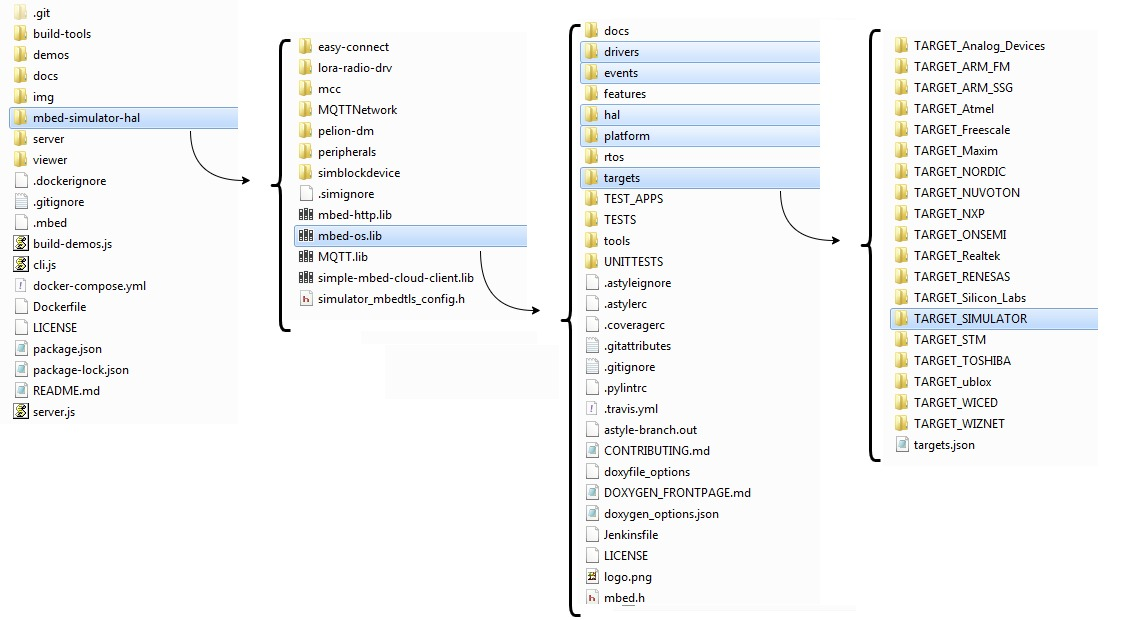
\includegraphics[scale=.37]{./Figures/estructuraMbed.jpg}
	\caption{Estructura de carpetas y archivos de \textit{Arm Mbed OS Simulator}.}
	\label{fig:estructuraMbed1}
\end{figure}
 
La carpeta \textquotedbl build-tools\textquotedbl{}  contiene tres archivos javascript: 

\begin{enumerate}
	\item build-application.js, que contiene funciones para construir aplicaciones en el contexto de \textit{Arm Mbed OS Simulator}. Asimismo, contiene métodos para encontrar los periféricos y manejar la construcción de componentes.
	
	\item build-libmbed.js, es un módulo de Node.js que realiza la compilación \textit{(build)} y gestión de dependencias. También, proporciona métodos que verifican las dependencias necesarias antes de la construcción.

	\item helpers.js,  es un módulo de Node.js que proporciona funciones relacionadas con operaciones de sistema de archivos, compilación, y manipulación de directorios y archivos.
\end{enumerate}
 
Dentro de la carpeta \textquotedbl demos\textquotedbl{}  se encuentran todos los programas ejemplo que muestran cómo utilizar ciertas funcionalidades de \textit{Arm Mbed OS Simulator} y son útiles como referencia para comenzar con el desarrollo en el entorno web. 
 
La carpeta \textquotedbl server\textquotedbl{}  contiene tres archivos javascript: 

\begin{enumerate}
	\item compile.js, este archivo realiza la generación de los archivos de salida compilados a partir del codigo fuente.
	
	\item get\_ips.js, proporciona una función para la configuración de las aplicaciones de red.

	\item launch-server.js, define y configura un servidor web que permite ejecutar solicitudes de ejecución de aplicaciones, gestionar las conexiones de red y la comunicación LoRaWAN.
	
\end{enumerate}
 
La carpeta \textquotedbl viewer\textquotedbl{}  contiene los archivos necesarios para crear interacción con el navegador. Entre estos archivos se encuentran: HTML, CSS, JavaScript, imágenes y bibliotecas de terceros o frameworks.
 
La carpeta \textquotedbl mbed-simulator-hal\textquotedbl{}  contiene las siguientes sub-carpetas y son usadas en el contexto de \textit{Arm Mbed OS Simulator}: 

\begin{itemize}
	\item easy-connect, dentro de esta carpeta se encuentran archivos que facilitan la conexión a una red utilizando Ethernet para manipular conexiones de red, sockets y eventos.
	
	\item lora-radio-drv, proporciona un marco para interactuar y controlar el módulo de radio LoRa, lo que permite enviar y recibir datos, administrar el estado y el funcionamiento.

	\item mcc, establece una cola de eventos que se utilizará para manejar eventos en \textit{Arm Mbed OS Simulator}. 
	
	\item MQTTNetwork, establece la interfaz para la comunicación de red con el protocolo MQTT. 
	
	\item pelion-dm, implementación de temporizadores y manejo de eventos para la plataforma mbed.
	
	\item peripherals, proporciona implementación de los periféricos externos para ejecutarse en el entorno web.
	
	\item simblockdevice, establece una interfaz para interactuar con  dispositivos de bloques que emula un dispositivo de almacenamiento físico en el navegador web.
	
	\item mbed-os.lib, es un archivo de biblioteca en formato binario que contiene la versión del código fuente del sistema operativo de Mbed OS  que usa \textit{Arm Mbed OS Simulator}.
	
\end{itemize}

La biblioteca \textquotedbl mbed-os.lib\textquotedbl{} se compone de las siguiente carpetas: 

\begin{itemize}

	\item drivers, dentro de esa carpeta se encuentran los diversos controladores que interactúan con los periféricos de hardware, y además, proporcionan una interfaz para acceder a ellos. 
	
	\item events, presenta archivos relacionados con la infraestructura de manejo de eventos para las tareas y operaciones de manera asíncrona.

	\item features, contiene varias subcarpetas con varios módulos que gestionan la conexión celular en dispositivos integrados, proporcionan una interfaz para interactuar con LoRaWAN, manejar la manipulación de memoria para el uso de la pila LWIP, proporciona mbed TLS, implementación del protocolo de red 6LoWPAN, sockets de red, comunicación inalámbrica de corto alcance entre dispositivos y almacenamiento de datos en sistemas embebidos. 
	
	\item hal, contiene implementaciones específicas de hardware para diferentes plataformas y microcontroladores.  
	
	\item platform, proporciona una capa de abstracción adicional sobre la capa de abstracción de hardware (HAL) .
	
	\item rtos, contiene la implementación del sistema operativo en tiempo real (RTOS).
	
	\item targets, cada sub-carpeta corresponde a un microcontrolador o una plataforma específica y, además, contiene información sobre cómo Mbed OS debe funciona con una plataforma en particular.
	
	\item TEST\_APPS, contiene ejemplos y aplicaciones de prueba de diferentes plataformas de hardware que se utilizan para probar y verificar diversas funcionalidades de Mbed OS.
	
	\item TESTS, contiene pruebas unitarias y de integración que verifican y validan el correcto funcionamiento de los módulos y características de Mbed OS.
	
	\item tools, contiene herramientas y utilidades para el desarrollo, compilación, depuración y prueba para diferentes plataformas de hardware y sistemas operativos.

	\item UNITTESTS, contiene pruebas unitarias para diferentes componentes del sistema operativo Mbed.

	\item mbed.h, este archivo contiene declaraciones y definiciones iniciales para que estén disponibles para el desarrollo web del usuario. 
	
\end{itemize}
 
\chapter{Diseño e implementación} % Main chapter title

\label{Chapter3} % Change X to a consecutive number; for referencing this chapter elsewhere, use \ref{ChapterX}

En este capítulo se exponen los criterios de selección para la arquitectura de la plataforma de emulación. Se presenta la arquitectura elegida y se describe la estructura y organización de las capas de programación.


\definecolor{mygreen}{rgb}{0,0.6,0}
\definecolor{mygray}{rgb}{0.5,0.5,0.5}
\definecolor{mymauve}{rgb}{0.58,0,0.82}

%%%%%%%%%%%%%%%%%%%%%%%%%%%%%%%%%%%%%%%%%%%%%%%%%%%%%%%%%%%%%%%%%%%%%%%%%%%%%
% parámetros para configurar el formato del código en los entornos lstlisting
%%%%%%%%%%%%%%%%%%%%%%%%%%%%%%%%%%%%%%%%%%%%%%%%%%%%%%%%%%%%%%%%%%%%%%%%%%%%%
\lstset{ %
  backgroundcolor=\color{white},   % choose the background color; you must add \usepackage{color} or \usepackage{xcolor}
  basicstyle=\footnotesize,        % the size of the fonts that are used for the code
  breakatwhitespace=false,         % sets if automatic breaks should only happen at whitespace
  breaklines=true,                 % sets automatic line breaking
  captionpos=b,                    % sets the caption-position to bottom
  commentstyle=\color{mygreen},    % comment style
  deletekeywords={...},            % if you want to delete keywords from the given language
  %escapeinside={\%*}{*)},          % if you want to add LaTeX within your code
  %extendedchars=true,              % lets you use non-ASCII characters; for 8-bits encodings only, does not work with UTF-8
  %frame=single,	                % adds a frame around the code
  keepspaces=true,                 % keeps spaces in text, useful for keeping indentation of code (possibly needs columns=flexible)
  keywordstyle=\color{blue},       % keyword style
  language=[ANSI]C,                % the language of the code
  %otherkeywords={*,...},           % if you want to add more keywords to the set
  numbers=left,                    % where to put the line-numbers; possible values are (none, left, right)
  numbersep=5pt,                   % how far the line-numbers are from the code
  numberstyle=\tiny\color{mygray}, % the style that is used for the line-numbers
  rulecolor=\color{black},         % if not set, the frame-color may be changed on line-breaks within not-black text (e.g. comments (green here))
  showspaces=false,                % show spaces everywhere adding particular underscores; it overrides 'showstringspaces'
  showstringspaces=false,          % underline spaces within strings only
  showtabs=false,                  % show tabs within strings adding particular underscores
  stepnumber=1,                    % the step between two line-numbers. If it's 1, each line will be numbered
  stringstyle=\color{mymauve},     % string literal style
  tabsize=2,	                   % sets default tabsize to 2 spaces
  title=\lstname,                  % show the filename of files included with \lstinputlisting; also try caption instead of title
  morecomment=[s]{/*}{*/}
}


%----------------------------------------------------------------------------------------
%	SECTION 1
%----------------------------------------------------------------------------------------
\section{Introducción}
 
Se investigó la arquitectura de \textit{Mbed Simulator} para adquirir una compresión del funcionamiento del \textit{Sistema Operativo Mbed}, de los periféricos simulados y las interacciones, además, de las configuraciones necesarias para la platadorma web.

Sin embargo, durante el análisis del repositorio, la presencia de múltiples módulos de código, bibliotecas y configuraciones que no estaban directamente relacionados con la simulación, inicialmente generó incertidumbre sobre su propósito y relevancia en la plataforma del simulador. En la figura \ref{fig:estructuraMbed} se exhibe la estructura de arbol de las carpetas y archivos de  \textit{Mbed Simulator} clonado desde GitHub.

\begin{figure}[ht]
	\centering
	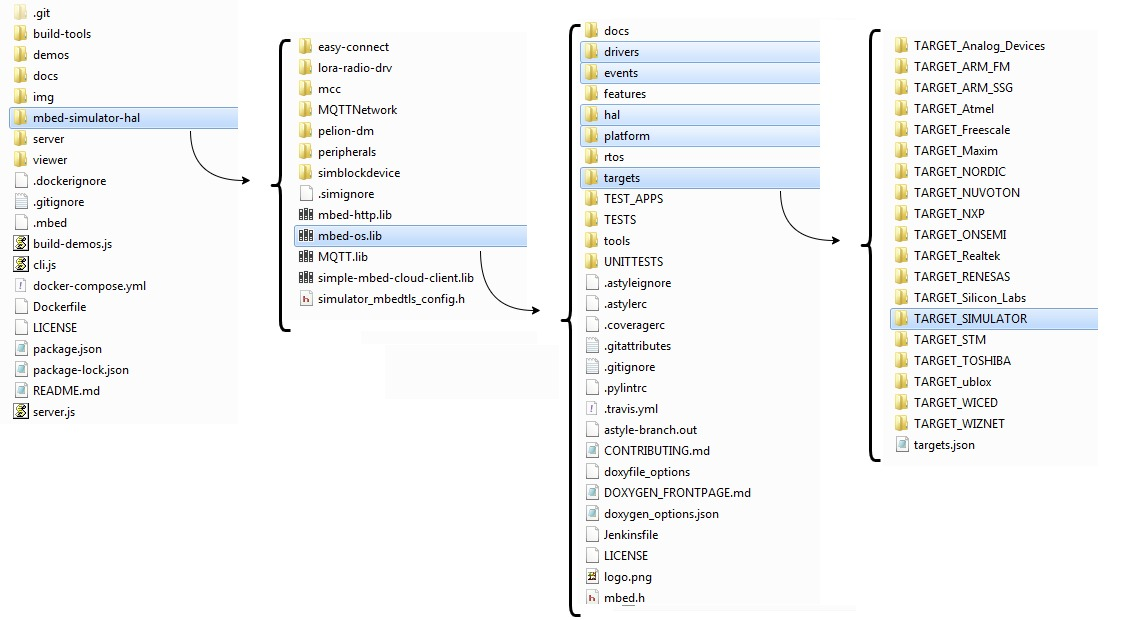
\includegraphics[scale=.35]{./Figures/estructuraMbed.jpg}
	\caption{Estructura de carpetas y archivos de \textit{Mbed Simulator}.}
	\label{fig:estructuraMbed}
\end{figure}
 
La carpeta \textquotedbl build-tools\textquotedbl contiene tres archivos javascript: 

\begin{enumerate}
	\item build-application.js, que contiene funciones para construir aplicaciones en el contexto de \textit{Mbed Simulator}. Asimismo, contiene métodos para encontrar los periféricos y manejar la construcción de componentes.
	
	\item build-libmbed.js, es un módulo de Node.js que realiza la construcción \textit{(build)} y gestión de dependencias. También, proporciona métodos que verifican las dependencias necesarias antes de la construcción.

	\item helpers.js,  es un módulo de Node.js que proporciona funciones relacionadas con operaciones de sistema de archivos, compilación, y manipulación de directorios y archivos.
\end{enumerate}
 
Dentro de la carpeta \textquotedbl demos\textquotedbl se encuentran todos los programas ejemplo que muestran cómo utilizar ciertas funcionalidades de \textit{Mbed Simulator} y son útiles como referencia para comenzar con el desarrollo en el entorno web. 
 
La carpeta \textquotedbl server\textquotedbl contiene tres archivos javascript: 

\begin{enumerate}
	\item compile.js, este archivo realiza la generación de los archivos de salida compilados a partir del codigo fuente.
	
	\item get\_ips.js, proporciona una función para la configuración de las aplicaciones de red.

	\item launch-server.js, define y configura un servidor web que permite ejecutar solicitudes de ejecución de aplicaciones, gestionar las conexiones de red y la comunicación LoRaWAN.
	
\end{enumerate}
 
La carpeta \textquotedbl viewer\textquotedbl contiene los archivos necesarios para crear interacción con el navegador. Entre estos archivos se encuentran: HTML, CSS, JavaScript, imágenes y bibliotecas de terceros o frameworks.
 
La carpeta \textquotedbl mbed-simulator-hal\textquotedbl contiene las siguiente sub-carpetas y son usadas en el contexto de \textit{Mbed Simulator}: 

\begin{itemize}
	\item easy-connect, dentro de esta carpeta se encuentran archivos que facilitan la conexión a una red utilizando Ethernet para manipular conexiones de red, sockets y eventos.
	
	\item lora-radio-drv, proporciona un marco para interactuar y controlar el módulo de radio LoRa, lo que permite enviar y recibir datos, administrar el estado y el funcionamiento.

	\item mcc, establece una cola de eventos que se utilizará para manejar eventos en \textit{Mbed Simulator}. 
	
	\item MQTTNetwork, establece la interfaz para la comunicación de red con el protocolo MQTT. 
	
	\item pelion-dm, implementación de temporizadores y manejo de eventos para la plataforma mbed.
	
	\item peripherals, proporciona implementación de los periféricos externos para ejecutarse en el entorno web.
	
	\item simblockdevice, establece una interfaz para interactuar con  dispositivos de bloques que emula un dispositivo de almacenamiento físico en el navegador web.
	
	\item mbed-os.lib, es un archivo de biblioteca en formato binario que contiene la versión del código fuente del sistema operativo de Mbed OS  que usa \textit{Mbed Simulator}.
	
\end{itemize}


Por consiguiente, la biblioteca \textquotedbl mbed-os.lib\textquotedbl contiene las siguiente carpetas: 

\begin{itemize}

	\item drivers, dentro de esa carpeta se encuentran los diversos controladores que interactúan con los periféricos de hardware, y además, proporcionan una interfaz para acceder a ellos. 
	
	\item events, presenta archivos relacionados con la infraestructura de manejo de eventos para las tareas y operaciones de manera asíncrona.

	\item features, contiene varias subcarpetas con varios módulos que gestionan la conexión celular en dispositivos integrados, proporcionan una interfaz para interactuar con LoRaWAN, manejar la manipulación de memoria para el uso de la pila LWIP, proporciona mbed TLS, implementación del protocolo de red 6LoWPAN, sockets de red, comunicación inalámbrica de corto alcance entre dispositivos y almacenamiento de datos en sistemas embebidos. 
	
	\item hal, contiene implementaciones específicas de hardware para diferentes plataformas y microcontroladores.  
	
	\item platform, proporciona una capa de abstracción adicional sobre la capa de abstracción de hardware (HAL) .
	
	\item rtos, contiene la implementación del sistema operativo en tiempo real (RTOS).
	
	\item targets, cada sub-carpeta corresponde a un microcontrolador o una plataforma específica y, además, contiene información sobre cómo Mbed OS debe funciona con una plataforma en particular.
	
	\item TEST\_APPS, contiene ejemplos y aplicaciones de prueba de diferentes plataformas de hardware que se utilizan para probar y verificar diversas funcionalidades de Mbed OS.
	
	\item TESTS, contiene pruebas unitarias y de integración que verifican y validan el correcto funcionamiento de los módulos y características de Mbed OS.
	
	\item tools, contiene herramientas y utilidades para el desarrollo, compilación, depuración y prueba para diferentes plataformas de hardware y sistemas operativos.

	\item UNITTESTS, contiene pruebas unitarias para diferentes componentes del sistema operativo Mbed.

	\item mbed.h, este archivo contiene declaraciones y definiciones iniciales para que estén disponibles para el desarrollo web del usuario. 
	
\end{itemize}


Después, al eliminar módulos y dependencias innecesarias, tales como: mbed-http, simple-mbed-cloud-client, features, rtos y todas las sub-carpetas dentro de la carpeta \textquotedbl target\textquotedbl excluyendo la sub-carpeta TARGET\_SIMULATOR, se procedió a evaluar la compatibilidad de su arquitectura. Durante el proceso, en primer lugar, se analizó si la arquitectura proporcionaba funcionalidades para la interacción con los usuarios. Incluso, de adaptarse fácilmente a futuros desarrollos y cambios, permitiendo un crecimiento escalable.

Además, la mantenibilidad y flexibilidad también fueron aspectos evaluados. Otro punto esencial, fueron las tecnologías y herramientas utilizadas, lo cual implicó una curva de aprendizaje adicional. 

Actualmente, \textit{Mbed Simulator} presenta las siguientes limitaciones:

\begin{enumerate}
	\item Dentro de un bucle infinito \texttt{while(1)}, es necesario agregar un retraso \newline(\texttt{delay)}, de lo contrario, el navegador no puede actualizar la interfaz de la plataforma web ni responder a eventos del usuario. Esto significa que el navegador no tiene la oportunidad de realizar otras tareas o responder a eventos mientras el bucle está en ejecución. Como resultado, el navegador se bloquea o congela y puede dejar de responder.
	
	\item En cada iteracion, la ejecución del programa puede variar en términos de tiempo, lo que puede afectar a la precisión en la sincronización de eventos dentro de la aplicación.

	\item En \textit{Mbed Simulator}, no hay restricciones significativas en cuanto a la cantidad de memoria que se puede asignar al stack o al heap  de un programa, lo cual difiere del hardware físico, donde sí existen limitaciones de memoria.
	
	\item Dentro del entorno web, las interrupciones no se manejan de la misma manera que en un sistema embebido real, debido a que no implementa el manejo de prioridades, por lo cual no afectan la ejecución del programa principal.
	
	\item Sin RTOS. No tiene la capacidad de ejecutar múltiples hilos de manera concurrente como lo haría un RTOS. Todo el código se ejecuta en un solo hilo. Se puede utilizar la biblioteca mbed-events para manejar ciertos aspectos de concurrencia, usando eventos y temporizadores.

\end{enumerate}

Finalmente, una vez confirmada su compatibilidad para los propósitos del presente trabajo, se tomó la decisión de seleccionarlo y empezar el desarrollo.


\section{Arquitectura de la plataforma web}

Después del análisis de \textit{Mbed Simulator}, se modificaron las carpetas y archivos de configuración para adaptarlos al entorno del emulador EDU-CIAA. Luego, se reemplazó \textquotedbl mbed-os\textquotedbl por la biblioteca \textit{\textbf{sAPI}}, pero se mantuvieron algunos componentes propios de Mbed, como \textquotedbl events\textquotedbl y \textquotedbl callback\textquotedbl, para agilizar el desarrollo.
  
En la figura \ref{fig:estructuraCiaa} se exhibe la estructura de las carpetas y archivos del  \textit{Emulador de la placa EDU-CIAA}.

\begin{figure}[ht]
	\centering
	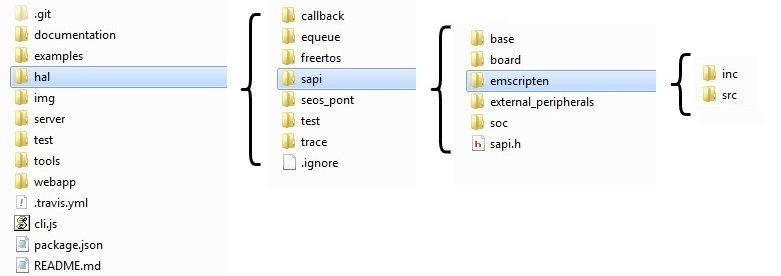
\includegraphics[scale=.50]{./Figures/estructuraCiaa.jpg}
	\caption{Estructura de carpetas y archivos de \textit{Mbed Simulator}.}
	\label{fig:estructuraCiaa}
\end{figure}
 

La emulación a nivel de API proporciona una capa de abstracción para el entorno de desarrollo del usuario, de modo que permite escribir aplicaciones en \textit{C} y ejecutarlas en la plataforma de emulación. 

Al utilizar esta capa de abstracción, se pudo replicar las funcionalidades y las características de configuración de la biblioteca \textit{\textbf{sAPI}} en un entorno diferente, en este caso, en un entorno web.


En el diagrama de bloques de la figura \ref{fig:Arquitectura} se muestra la arquitectura básica de una aplicación de usuario que ejecuta el emulador de la placa EDU-CIAA-NXP.


\begin{figure}[ht]
	\centering
	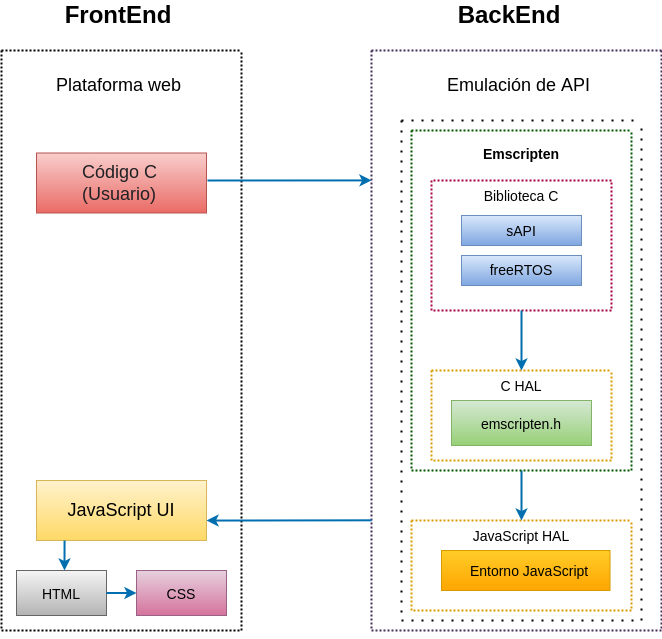
\includegraphics[scale=.55]{./Figures/Arquitectura.png}
	\caption{Diagrama de bloques arquitectura de la plataforma.}
	\label{fig:Arquitectura}
\end{figure}

A continuación, se presenta una breve descripción de cada componente del diagrama de bloques de la figura \ref{fig:Arquitectura}:

\begin{enumerate}
	\item El usuario escribe un programa en código de lenguaje \textit{C}, que utiliza la biblioteca \textit{\textbf{sAPI}} u otras. 
	
	\item El código del usuario se conecta a través de la plataforma de emulación con la capa 
\textit{Biblioteca C}, que proporciona la emulación a nivel de API de la biblioteca \textit{\textbf{sAPI}}.
	
	\item La capa \textit{Biblioteca C} se comunica con la capa \textit{C HAL} (capa abstracción de hardware) escrita en \textit{C}. Esta capa \textit{C HAL} proporciona las definiciones necesarias para que el compilador de \textit{Emscripten} traduzca el código escrito en lenguaje \textit{C} a código que puede ser ejecutado en el entorno web.
	
	\item La capa \textit{JavaScript HAL} se comunica con la capa \textit{C HAL}  a través de los archivos \textit{WebAssembly} y \textit{JavaScript} generados por el proceso de compilación de \textit{Emscripten}.
	
	\item La capa de abstracción de JavaScript (\textit{JavaScript HAL}) actúa como intermediario entre las capa \textit{C HAL} y la interfaz de usuario en \textit{JavaScript} (\textit{JavaScript UI}). Y además, se encarga de distribuir eventos y llamadas entre ambas capas.
	
\item La interfaz de usuario en \textit{JavaScript} (\textit{JavaScript UI}) maneja los eventos procedentes de la capa \textit{JavaScript HAL}. No interactúa directamente con el código \textit{JavaScript} y \textit{WebAssembly} resultante del código \textit{C}.

\item La capa \textit{JavaScript UI} accede y modifica dinámicamente los elementos HTML, que utilizan reglas de estilo \textit{CSS} para la presentación en la plataforma web.
	
\end{enumerate}


En resumen, el diagrama representa cómo un programa escrito en lenguaje \textit{C} interactúa con la capa de abstracción de la emulación a nivel de API hasta llegar a la interfaz de usuario en \textit{JavaScript}. La compilación con \textit{Emscripten} permite que el código en \textit{C} se ejecute en el navegador web, lo que posibilita la ejecución del programa de usuario en un entorno basado en la web.


\section{Frontend}
En esta parte de la plataforma web se implementó el desarrollo de la interacción entre el \textit{backend} y el navegador del usuario.


\subsection{Diseño de la Interfaz de Usuario}

Para el desarrollo de la interfaz, se optó por un diseño intuitivo, de manera que el usuario se sienta familiarizado con las herramientas de trabajo y que la disposición de los componentes sea cómoda y esté organizada al momento de usarlas.

La figura \ref{fig:PlataformaEmulador1} muestra la plataforma web del Emulador de la placa EDU-CIAA-NXP.

\begin{figure}[ht]
	\centering
	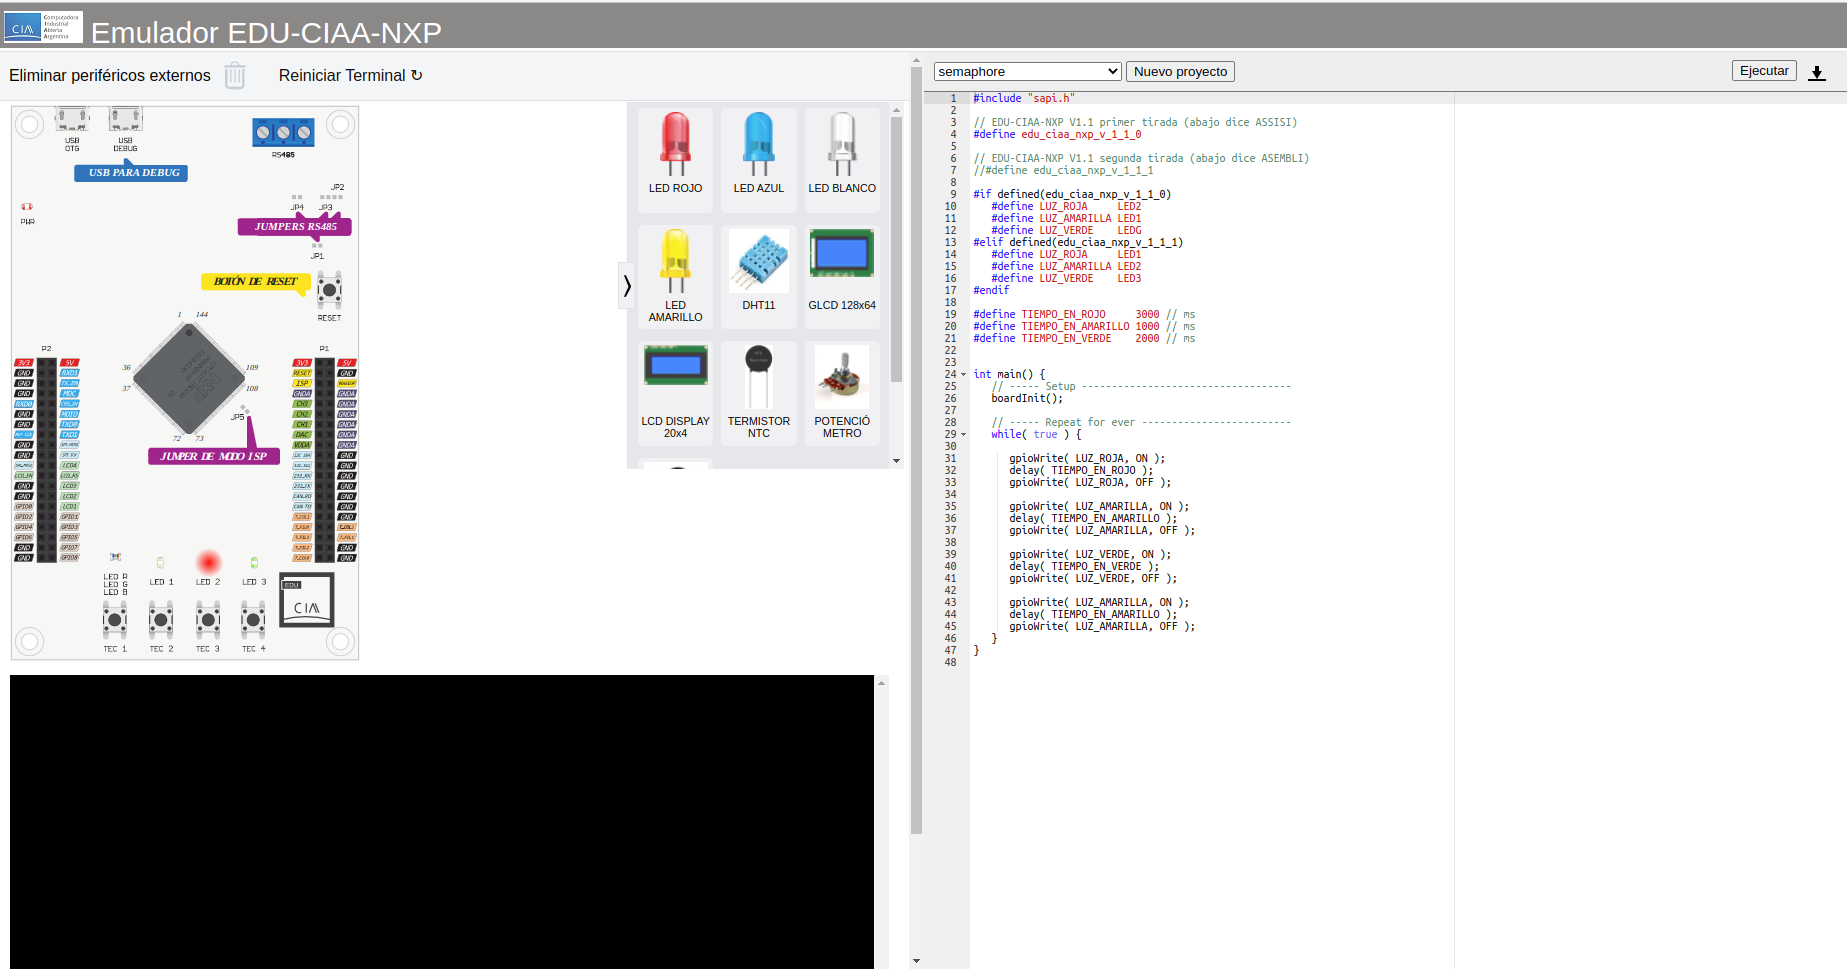
\includegraphics[scale=.20]{./Figures/PlataformaEmulador.png}
	\caption{Plataforma de emulación para la placa EDU-CIAA-NXP.}
	\label{fig:PlataformaEmulador1}
\end{figure}


Para su estudio, dividimos la plataforma web en tres partes. En la figura \ref{fig:PlataformaEmulador2}, se muestra la parte izquierda y superior de la interfaz gráfica para interactuar con el hardware. La figura \ref{fig:PlataformaEmulador3} muestra la parte inferior izquierda, donde se visualiza la salida de la consola. Finalmente, en la figura \ref{fig:PlataformaEmulador4}, se muestra la parte derecha de la interfaz gráfica destinada a la aplicación de usuario.

\begin{figure}[ht]
	\centering
	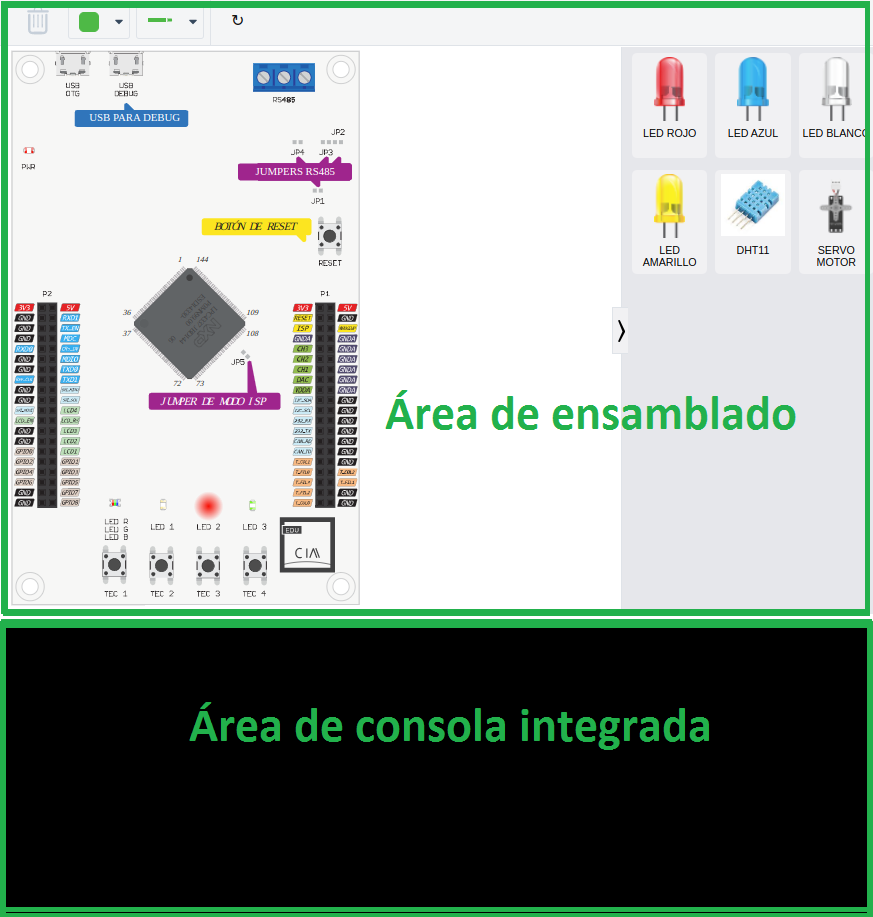
\includegraphics[scale=.57]{./Figures/PlataformaEmulador1.png}
	\caption{Parte izquierda y superior de la plataforma de emulación de la placa EDU-CIAA-NXP.}
	\label{fig:PlataformaEmulador2}
\end{figure}


\begin{figure}[ht]
	\centering
	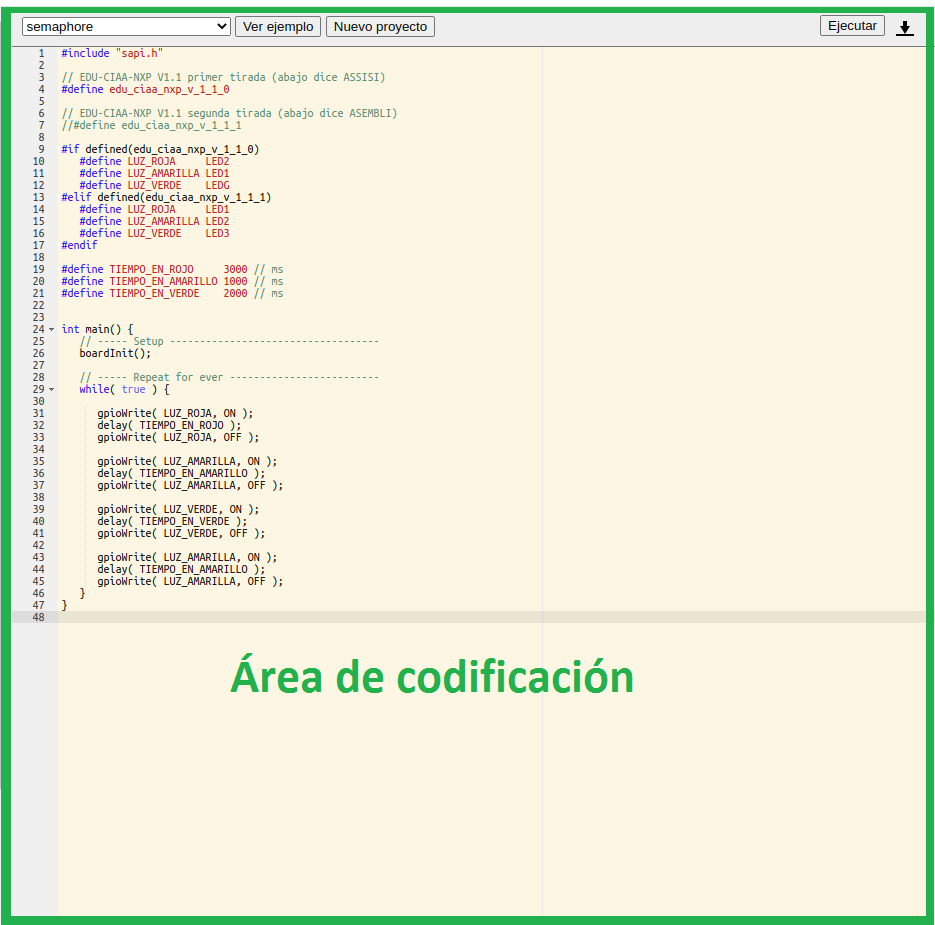
\includegraphics[scale=.58]{./Figures/PlataformaEmulador2.png}
	\caption{Parte inferior izquierda de la plataforma de emulación de la placa EDU-CIAA-NXP.}
	\label{fig:PlataformaEmulador3}
\end{figure}


\hfill \break
\hfill \break
\hfill \break
\hfill \break
\hfill \break
\hfill \break
\hfill \break

\begin{figure}[ht]
	\centering
	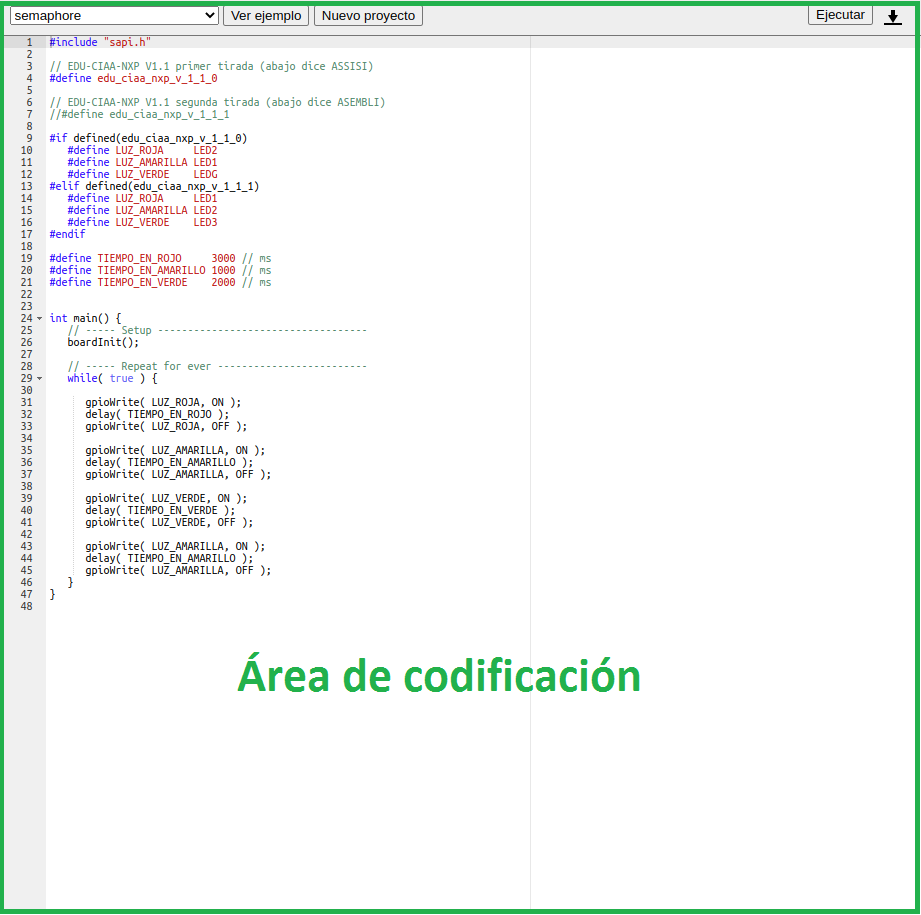
\includegraphics[scale=.55]{./Figures/PlataformaEmulador3.png}
	\caption{Parte derecha de la plataforma de emulación de la placa EDU-CIAA-NXP.}
	\label{fig:PlataformaEmulador4}
\end{figure}

Por consiguiente, el diseño de la interfaz de usuario de la plataforma proporciona las siguientes áreas:

\begin{itemize}
	\item Área de ensamblado: el valor predeterminado muestra la placa EDU-CIAA-NXP, y también se permite agregar componentes.
	\item Área de codificación: se proporciona un editor de código en línea para programar con la placa EDU-CIAA-NXP. La primera vez que se accede a la platafoma se muestra en ejecución un ejemplo de código predeterminado.
	\item Área de consola integrada: se muestra en una ventana la salida que se vería a través del puerto serie. 
\end{itemize}


Debido a las áreas de trabajo que presenta la plataforma, el
usuario programador podrá realizar las siguientes tareas:

\begin{itemize}
	\item Ver los programas de ejemplo predeterminados.
	\item Crear un nuevo proyecto.
	\item Ejecutar un programa de ejemplo o uno nuevo.
	\item Editar programas.
	\item Visualizar los cambios programados para la placa virtual.
	\item Agregar nuevos componentes.
	\item Ver los errores obtenidos en la programación.
	\item Ver lo programado en la salida de consola.
\end{itemize}

\subsubsection{Área de ensamblado}

Para el desarrollo de la placa EDU-CIAA-NXP y componentes externos se usaron dibujos en formato de gráficos vectoriales bidimensionales (SVG) por las siguientes características:

\begin{itemize}
	\item Son más ligeras, entonces se cargan más rápido en el navegador.
    \item Por su capacidad de ser modificado por medio de \textit{JavaScript}. Por lo tanto, se pudieron crear imágenes interactivas.
	\item Evitan que las imagenes se deformen y no pierden calidad.
	\item Permite programar animaciones.
\end{itemize}

En ese sentido, para la capa de programación \textit{JavaScript UI}, se pudo implementar el comportamiento interactivo para los botones de la placa (TEC1, TEC2, TEC3 y TEC4) usando el código SVG generado para la placa EDU-CIAA-NXP, incluso, se pudo modificar también el comportamiento de los LEDs, que permitió mostrar dinamicamente en la placa el encendido y apagado.

Además, con el objetivo de optimizar la experiencia del usuario, esta área permite elegir uno o más dispositivos virtuales de entrada/salida desde la barra lateral \textit{sidebars} derecho. En esta barra se exhiben todos los periféricos disponibles para la plataforma web. 

Una vez que el usuario elige un periférico de la barra lateral y realiza la configuración de las conexiones, la barra automáticamente colapsa, ocultándose del área de ensamblado. Al colapsarse, se muestra el periférico integrado en la aplicación. Asimismo,  el usuario tiene la opción de volver a expandir la barra lateral para agregar un nuevo periférico.

También, cuando se añadió un periférico virtual, el usuario tiene la posibilidad de eliminarlo. Para realizarlo, simplemente debe seleccionar el periférico deseado, lo que habilitará el icono de \textquotedbl Eliminar periféricos externos\textquotedbl. Al hacer clic en el icono, el periférico virtual será eliminado de forma automática y efectiva.


En la figura \ref{fig:AgregarPeriferico} se observa que el usuario puede elegir qué componente agregar a la aplicación y en la figura \ref{fig:AgregarPeriferico2} se muestra que el componente se agregó a la aplicación.
\hfill \break
\hfill \break
\hfill \break
\hfill \break
\hfill \break
\hfill \break
\hfill \break
\hfill \break
\hfill \break
\hfill \break
\hfill \break
\hfill \break
\hfill \break



\begin{figure}[ht]
	\centering
	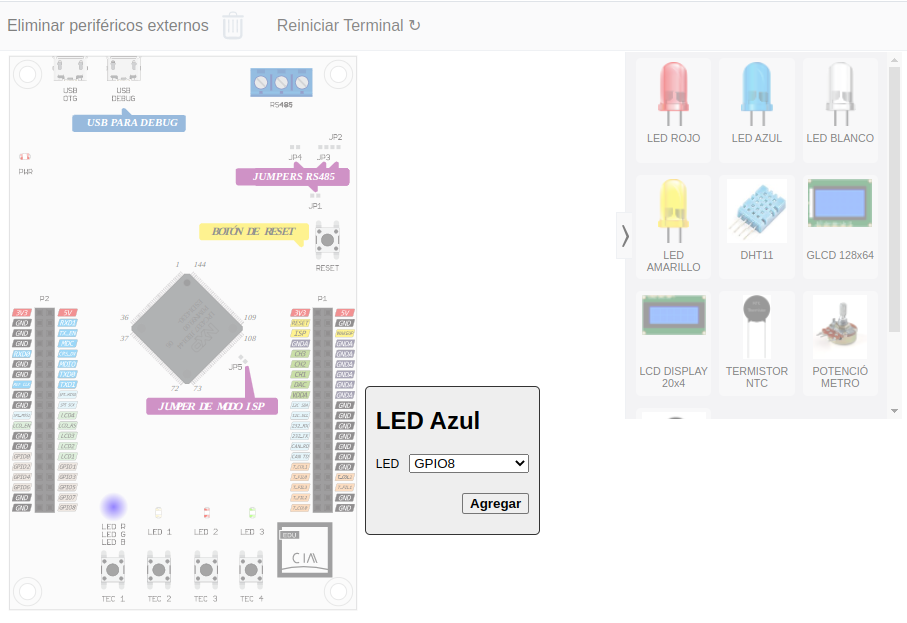
\includegraphics[scale=.33]{./Figures/AgregarPeriferico.png}
	\caption{Agregar periférico.}
	\label{fig:AgregarPeriferico}
\end{figure}


\begin{figure}[ht]
	\centering
	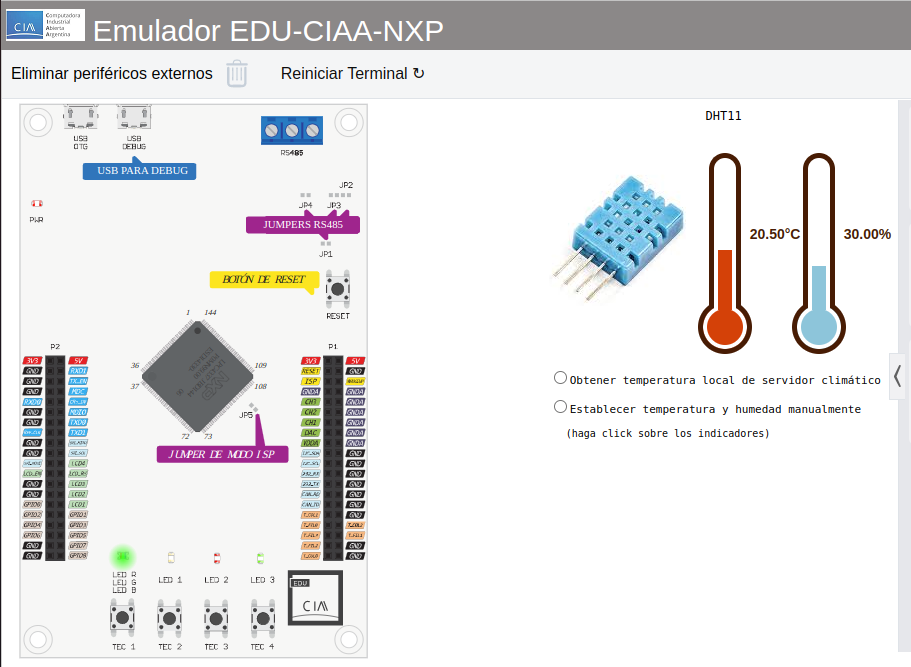
\includegraphics[scale=.33]{./Figures/AgregarPeriferico2.png}
	\caption{Periférico agregado en el área de ensamblado. }
	\label{fig:AgregarPeriferico2}
\end{figure}


\subsubsection{Área de codificación}

Esta parte de la plataforma se reserva al usuario para que pueda programar sus propias aplicaciones. Esta ventana de edición presenta las siguientes capacidades:

\begin{itemize}
\item Manejar la sintaxis para el lenguaje C.
\item Soportar el uso de las constantes, como por ejemplo: '\#define'.
\item Permitir el uso de las palabras claves, comentarios, etc.
\item Permitir el resaltado de líneas de código, sangría automática y número de línea.
\item Utilizar la función buscar (ctrl + f).
\item Utilizar la función buscar/reemplazar (ctrl + h).
\item Utilizar la función rehacer (ctrl + y).
\end{itemize}


Para compilar un programa, la plataforma provee al usuario el botón “ejecutar”. Sin embargo, si hubo problemas de sintaxis, errores lógicos, etc., se mostrarán esos errores al usuario.

En la figura \ref{fig:PlataformaErrores2} se muestra el código que generó los errores de compilación y en la figura \ref{fig:PlataformaErrores1} se observa los errores de compilación en el área de ensamblado.



\begin{figure}[ht]
	\centering
	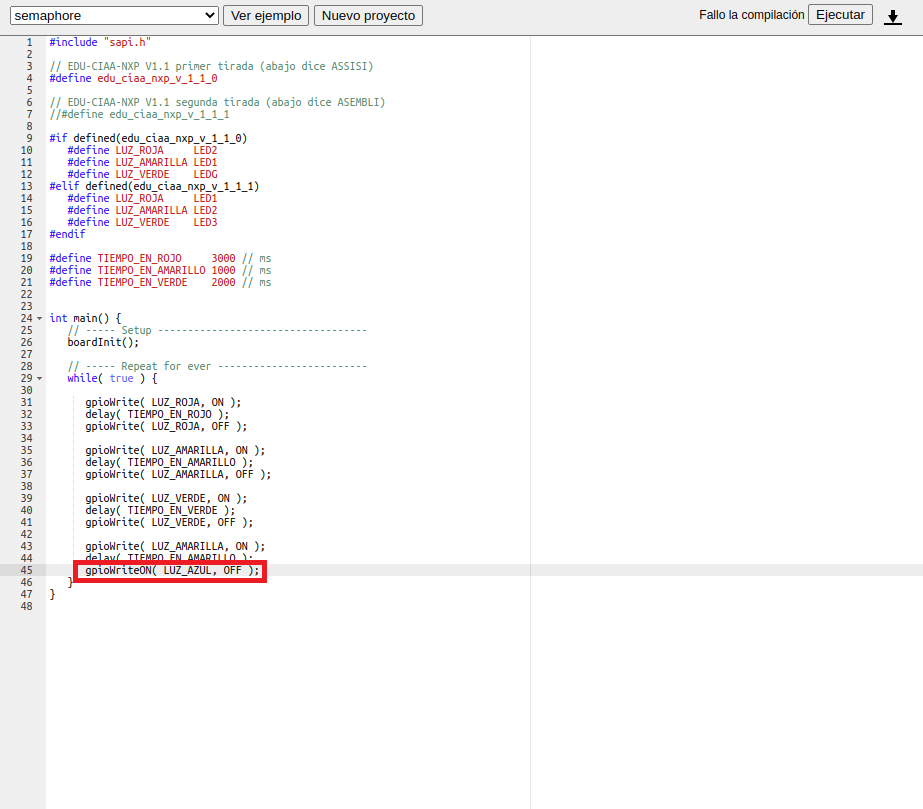
\includegraphics[scale=.39]{./Figures/PlataformaErrores1.png}
	\caption{Código que generó los errores de compilación.}
	\label{fig:PlataformaErrores2}
\end{figure}



\begin{figure}[ht]
	\centering
	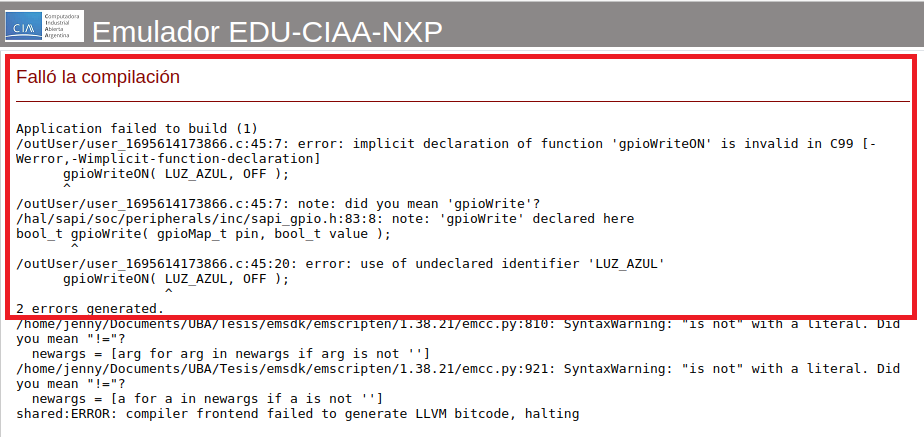
\includegraphics[scale=.39]{./Figures/PlataformaErrores2.png}
	\caption{Errores de compilación.}
	\label{fig:PlataformaErrores1}
\end{figure}

También, se implementó una estructura jerárquica en la lista desplegable de ejemplos. El propósito es organizar y presentar los ejemplos agrupados por periféricos, de manera más ordenada y fácil de navegar para el usuario.

La figura \ref{fig:listExamples} muestra la estructura jerárquica de la lista de ejemplos.

\begin{figure}[ht]
	\centering
	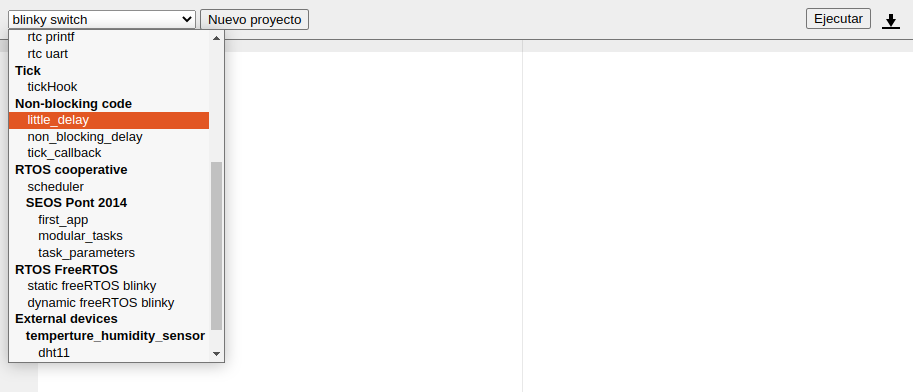
\includegraphics[scale=.42]{./Figures/listExamples.jpg}
	\caption{Estructura jerárquica de ejemplos. }
	\label{fig:listExamples}
\end{figure}

Ademas, al seleccionar algún ejemplo que contiene un periférico externo de la lista desplegable, la aplicación, automáticamente cargara dentro del área de ensamblado el periférico con las conexiones a los pines configurados por defecto. Es decir, el usuario no tendrá la necesidad de seleccionar y configurar el periférico desde la barra lateral del área de ensamblado.

La figura \ref{fig:cargarPeriferico} muestra el periférico agregado automáticamente al seleccionar el ejemplo \textquotedbl potentiometer\textquotedbl.

\begin{figure}[ht]
	\centering
	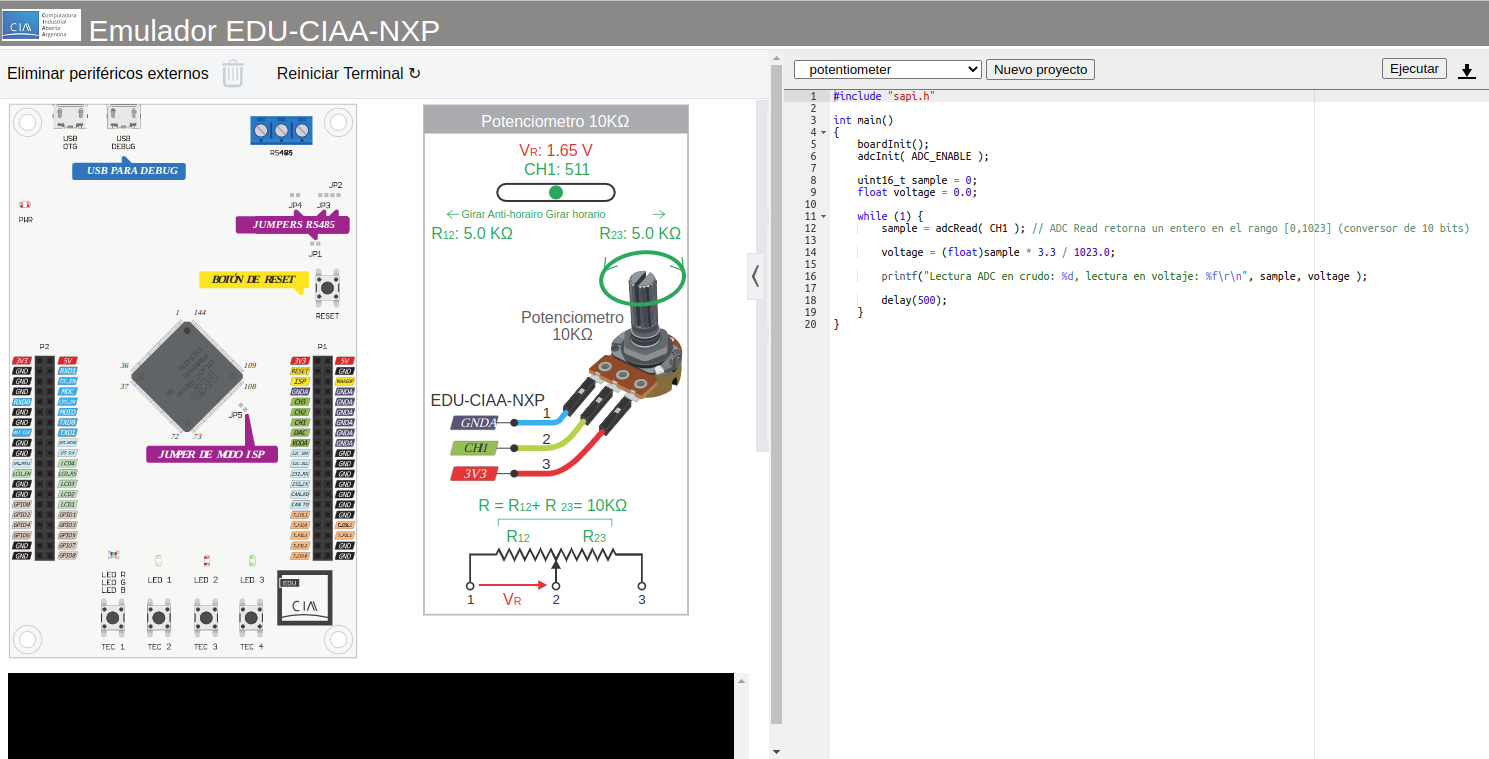
\includegraphics[scale=.21]{./Figures/cargarPeriferico.png}
	\caption{Carga automática del Periférico. }
	\label{fig:cargarPeriferico}
\end{figure}



\subsubsection{Área de consola integrada}

Dentro del código traducido en el proceso de compilación por \textit{Emscripten}, se encuentran las siguientes funciones definidas y configuradas previamente, las cuales son: 

\begin{itemize}
\item \texttt{print}, esta función envía el texto a la terminal de la interfaz gráfica del emulador web, al utilizar la función \texttt{terminal.write}.
\item \texttt{printErr}, se comunica con la consola de error del navegador, al usar \newline \texttt{console.error}.
\end{itemize}

Ambas funciones interactuan con el código \textit{JavaScript}. La función \texttt{printErr} se comunica con la consola de error del navegador y la función \texttt{print} se comunica con la terminal del emulador web a través de la biblioteca xterm.js, que es un componente de terminal de front-end escrito en \textit{JavaScript} y que permite construir terminales en el navegador. 

Entre las principales características de xterm.js se destaca:

\begin{itemize}
	\item Funciona con la mayoría de las aplicaciones de terminal, como bash, es compatible con aplicaciones basadas y eventos de mouse.
	\item Es de alto rendimiento, por eso es realmente rápido.
	\item No requiere de dependencias externas para funcionar, sin embargo, la dependencia principal para el funcionamiento básico es el propio navegador web.
	\item API bien documentada.
\end{itemize}


Además de las características de Xterm.js, esta biblioteca de \textit{JavaScript} es usado por varios proyectos populares como VS Code, Hyper y Theia que lo usan, de ahí que, el soporte en la comunidad de desarrolladores es amplio.

En la figura \ref{fig:Terminal2} se puede observar la salida por consola de un programa.

\begin{figure}[ht]
	\centering
	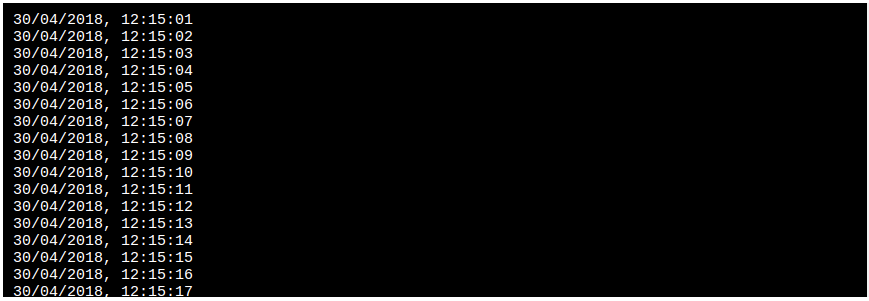
\includegraphics[scale=.60]{./Figures/Terminal2.png}
	\caption{Salida de la terminal serie.}
	\label{fig:Terminal2}
\end{figure}

Y en la figura \ref{fig:Terminal1} se muestra el programa de usuario que generó la salida por consola.

\begin{figure}[ht]
	\centering
	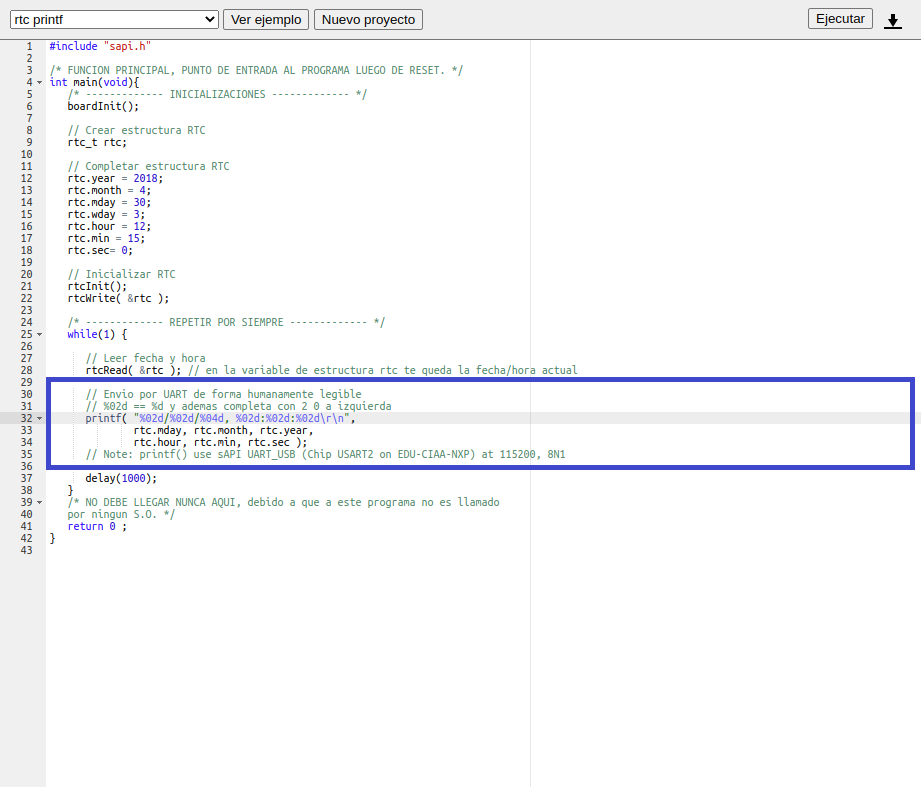
\includegraphics[scale=.41]{./Figures/Terminal1.png}
	\caption{Programa de usuario que imprime por consola.}
	\label{fig:Terminal1}
\end{figure}
 



 
 

\subsection{JavaScript UI}

Esta capa se desarrolló con el propósito de que se comunique con la capa \textit{JavaScript HAL}, y también con el objetivo de proporcionar componentes de código, utilidades y manejo de eventos en la aplicación de usuario.

Por tanto, para lograr la comunicación con la capa \textit{JavaScript HAL}, se desarrolló en esta capa los objetos que se sucriben al detector de eventos programados en la \textit{HAL}.

\textit{JavaScript} permite crear oyentes, utilizando el método \texttt{on()} y pasando como argumento el nombre del evento al que se quiere suscribir. De esta manera, se  programaron varios subscriptores para un mismo evento en diferentes archivos \textit{JavaScript} dentro de esta capa. En consecuencia, se logró una mayor interactividad entre los componentes de la plataforma.

Es decir, cuando se emite algún evento en la \textit{HAL}, entonces el oyente suscrito a ese evento en esta capa \textit{UI} lo podrá escuchar y realizar las acciones que correspondan para la funcionalidad requerida. La figura \ref{fig:EventemitterNodeJSUI} describe esta situación.

\hfill \break
\hfill \break
\hfill \break
\hfill \break
\hfill \break
\hfill \break
\hfill \break
\hfill \break

\begin{figure}[ht]
	\centering
	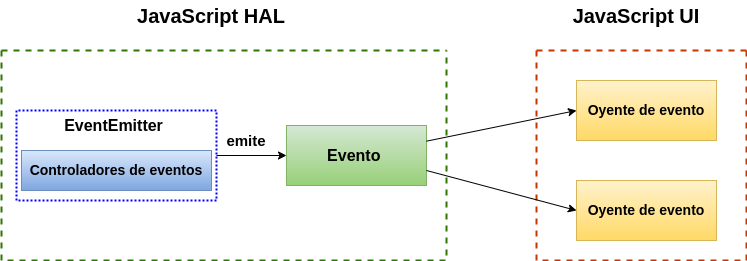
\includegraphics[scale=.52]{./Figures/EventemitterNodeJSUI.png}
	\caption{Diagrama de bloques de los oyentes de \textit{EventEmitter} en la capa UI.}
	\label{fig:EventemitterNodeJSUI}
\end{figure}




\subsection{Aplicación de Usuario}
La plataforma de emulación para la placa EDU-CIAA-NXP es una aplicación en línea, que se ejecuta en el \textit{browser} del usuario. La interfaz fue diseñada como una herramienta que permite al usuario realizar sus tareas de programación dentro de una plataforma simple e intuitiva.

Sin embargo, existen algunas limitaciones que se deben tener en cuenta.

\begin{itemize}
	\item Las unidades de tiempo especificadas por los valores en las constantes, por ejemplo cuando el usuario define \texttt{TASK1\_PERIODICITY} con un valor de 1000 para ser usado dentro del codigo siguiente: 
	
\begin{lstlisting}[caption={Ejemplo TASK1\_PERIODICITY}]
#define TASK1_PERIODICITY 1000} 

if( task1Counter++ == TASK1_PERIODICITY ){
  task1();
  task1Counter = 0;
}
\end{lstlisting}	
	


Significa que la tarea  planificada se ejecutará cada 1000 milisegundos en la placa fisica. Sin embargo, en el emulador web, la velocidad de ejecución puede variar y no necesariamente coincidir con el tiempo real. Por lo tanto, el tiempo de ejecución de cada iteración de la tarea \texttt{task1} podría ser más lento en el emulador web. Estas diferencias en la ejecución se deben a las limitaciones inherentes de \textit{JavaScript} y \textit{Emscripten}, que pueden afectar la precisión del tiempo.

\end{itemize}

\section{Backend}

En esta capa de programación se desarrolló toda la lógica necesaria para emular las funcionalidades que proporcionan las bibliotecas: \textit{\textbf{sAPI}}, \textit{\textbf{freertos}} y \textit{\textbf{seos\textunderscore pont}} para la placa EDU-CIAA-NXP.

\hfill \break
\hfill \break
\hfill \break


\subsection{Biblioteca C}

En primer lugar, se identificaron las funciones de las bibliotecas \textit{C} originales para empezar a emular. Luego, en el emulador se crearon interfaces que reflejen las estructuras de las bibliotecas originales, que incluyo definiciones de funciones, estructuras de datos y constantes.

Es decir, en las funciones originales se examinaron los parámetros de entrada y los valores de retorno, para luego mapearlos correctamente en las definiciones de las funciones del emulador.  A modo de referencia se muestra en la tabla \ref{tab:gpioMap} las definiciones de las funciones para \texttt{sapi\_gpio.h}, que incluye los nombres de la funciones, los tipos de parámetros y el tipo de valor de retorno. Cabe destacar que estas definiciones son idénticas tanto en las \textit{\textbf{sAPI}} como en el emulador, lo que permite una fácil correspondencia entre ambas.


\begin{table}[h]
	\centering
	\caption[Módulo \textit{GPIO}]{Módulo \textit{GPIO}}
	\begin{tabular}{l c c}    
		\toprule
		\textbf{Nombre de la función} 	 & \textbf{Parámetros} 		& \textbf{Tipo de retorno}  \\
		\midrule
		gpioInit & gpioMap\_t, gpioInit				&  bool\_t \\		
		gpioRead	 & gpioMap\_t				&  bool\_t \\
		gpioWrite	 & gpioMap\_t, bool\_t				&  bool\_t \\
		gpioToggle	 & gpioMap\_t				&  bool\_t \\
		\bottomrule
		\hline
	\end{tabular}
	\label{tab:gpioMap}
\end{table}



Al igual que en la biblioteca \textit{\textbf{sAPI}} del proyecto CIAA, los archivos de código fuente para la plataforma de emulación, conservan el mismo nombre, por ejemplo  \texttt{sapi\_gpio.c}. Sin embargo, la implementación de las funciones es totalmente distinta. En el caso de la biblioteca \textit{\textbf{sAPI}} del proyecto CIAA, para \texttt{sapi\_gpio.c}  se incluyen los archivos de encabezado: \texttt{gpio\_18xx\_43xx.h} y \newline \texttt{scu\_18xx\_43xx.h}. Y en el caso de la plataforma de emulación se usa otro archivos de encabezado como \texttt{gpio\_api.h} para replicar el mismo comportamiento.

A continuación, se presenta una comparación entre las clases del módulo GPIO de la biblioteca \textit{\textbf{sAPI}} del proyecto CIAA y el módulo GPIO implementado en la plataforma de emulación. 

La figura \ref{fig:GPIOsAPI} muestra las dependencias que se usan para la implementación de \newline \texttt{sapi\_gpio.c} del proyecto CIAA y en la figura \ref{fig:GPIOEmulador} se muestran las dependencias utilizadas en el emulador para el mismo módulo, logrando el \textit{port} al emulador de las funciones para el manejo del periférico GPIO.


\hfill \break
\hfill \break
\hfill \break
\hfill \break
\hfill \break
\hfill \break
\hfill \break
\hfill \break
\hfill \break
\hfill \break
\hfill \break
\hfill \break

\begin{figure}[ht]
	\centering
	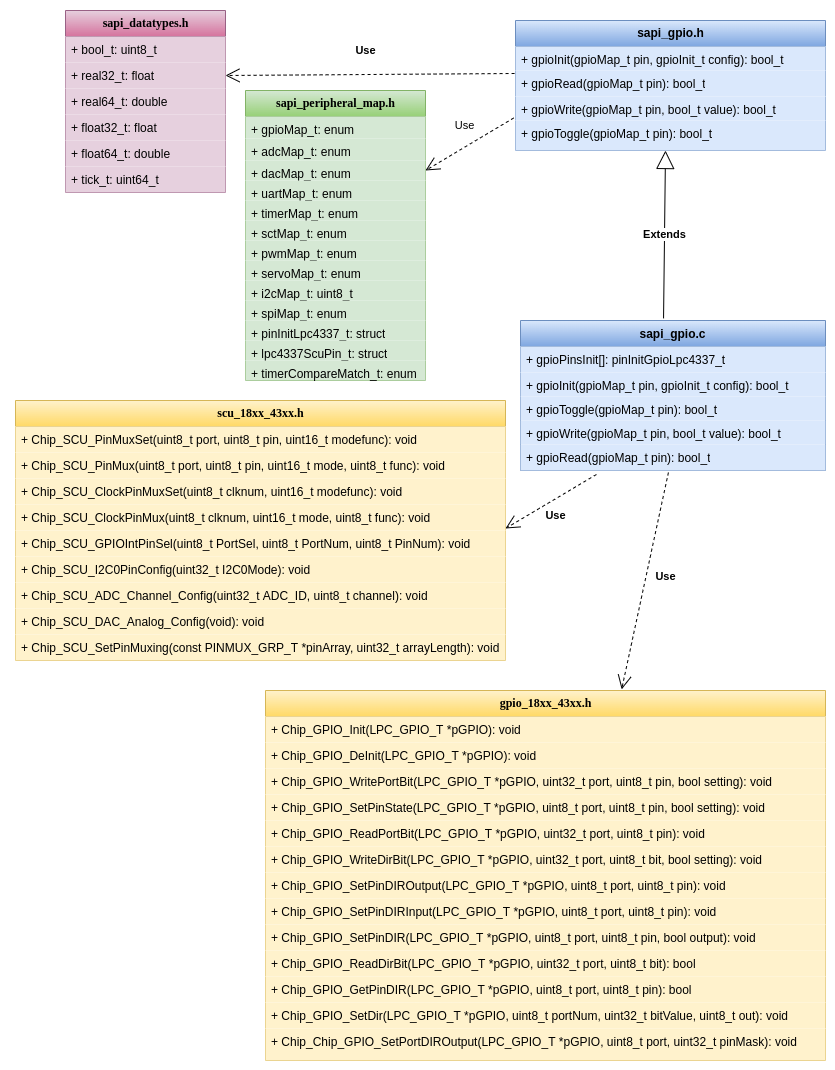
\includegraphics[scale=.41]{./Figures/DiagramaClasesGPIOsAPI.png}
	\caption{Diagrama de dependencias del módulo \textit{GPIO} de la biblioteca \textit{\textbf{sAPI}} del proyecto CIAA.}
	\label{fig:GPIOsAPI}
\end{figure}


\hfill \break
\hfill \break
\hfill \break
\hfill \break
\hfill \break
\hfill \break
\hfill \break
\hfill \break
\hfill \break
\hfill \break
\hfill \break
\hfill \break


\begin{figure}[ht]
	\centering
	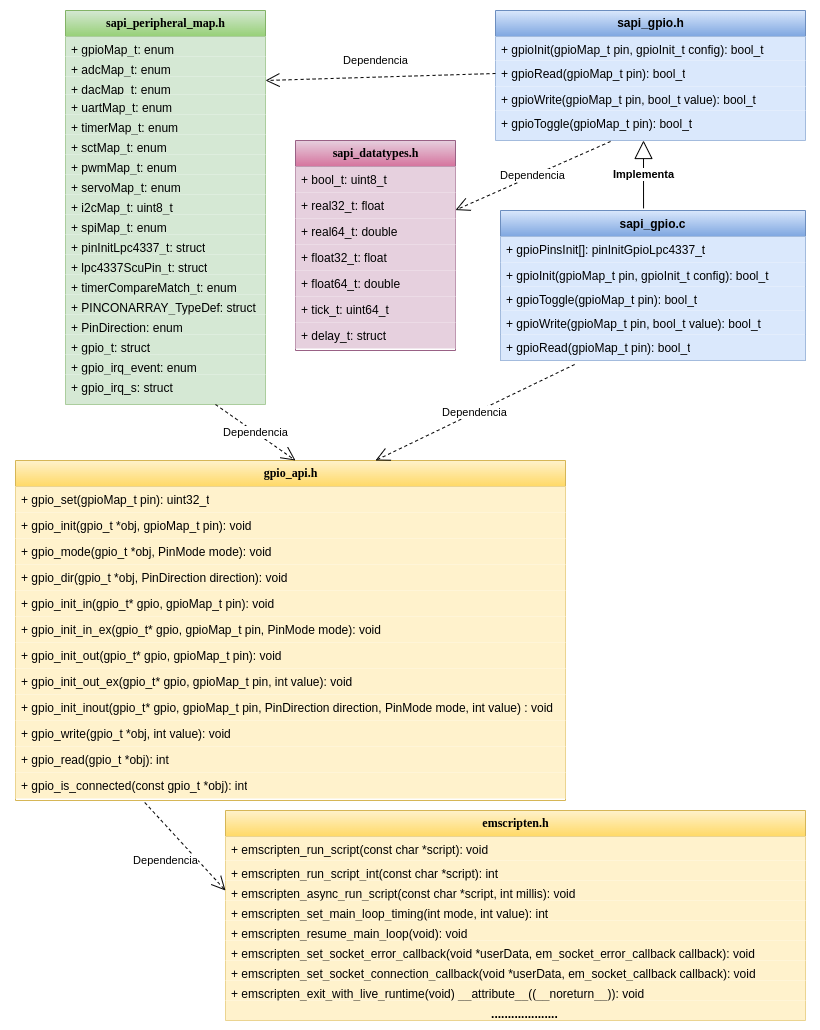
\includegraphics[scale=.41]{./Figures/DiagramaClasesEmulador.png}
	\caption{Diagrama de dependencias del módulo \textit{GPIO} de la plataforma de emulación para la placa EDU-CIAA-NXP.}
	\label{fig:GPIOEmulador}
\end{figure}


Para todos los demás módulos de la biblioteca \textit{\textbf{sAPI}} para la pogramación de periféricos del microcontrolador se siguió esta misma lógica. Asimismo, se utilizó un esquema de nomenclatura de los archivos de encabezado y de código fuente similar al de las bibliotecas originales.  Esto permitió mantener una estructura organizada y coherente en la emulación, que facilita el mantenimiento y comprensión.


También, se reutilizó el archivo de encabezado \texttt{sapi.h} que cumple con la misma funcionalidad que en la biblioteca \textit{\textbf{sAPI}}, la cual consiste en incluir todos los módulos que conforman la biblioteca para utilizarla en el programa de usuario. 

Además, se reutilizaron los archivos de encabezado: \texttt{sapi\_datatypes.h} y \newline \texttt{sapi\_peripheral\_map.h} incluidos en todos los módulos de la biblioteca \textit{\textbf{sAPI}} del proyecto CIAA. La decisión de reutilización fue para emular las características de hardware y prevalecer el uso de todos los tipos de datos básicos y configuraciones de la placa.

En la tabla \ref{tab:ConfiguracionGPIO} se muestran los tipos de datos de \texttt{sapi\_peripheral\_map.h} que se usan en la plataforma de emulación. Se puede observar que se reutilizó los nombres: TEC1, TEC2, TEC3 y TEC4 para los botones y los nombres LEDR, LEDG, LEDB, LED1, LED2 y LED3 para los LEDs de la placa EDU-CIAA-NXP.

\begin{table}[h]
	\centering
	\caption[\texttt{sapi\_peripheral\_map.h}.]{Tipos de datos de \texttt{sapi\_peripheral\_map.h} que se reutilizan en en la plataforma de emulación.}
	\begin{tabular}{l c c c}    
		\toprule
		\textbf{P2 header} & \textbf{P1 header} & \textbf{LEDs}  & \textbf{Switches}\\
		\midrule
		GPIO8, GPIO7, GPIO5 & T\_FIL1 &  LEDR &  TEC1\\		
		GPIO3, GPIO1, LCD1 & T\_COL2  & LEDG &  TEC2\\
		LCD2, LCD3, LCDRS & T\_COL0 & LEDB &  TEC3\\
		LCD4, SPI\_MISO, ENET\_TXD1 & T\_FIL2 & LED1 & TEC4\\
		ENET\_TXD0, ENET\_MDIO, ENET\_CRS\_DV & T\_FIL3 & LED2 & \\
	    ENET\_MDC, ENET\_TXEN, ENET\_RXD1 & T\_FIL0 & LED3 & \\
	    GPIO6, GPIO4, GPIO2 & T\_COL1&  & \\
	    GPIO0, LCDEN, SPI\_MOSI, ENET\_RXD0 & CAN\_TD&  & \\
		\bottomrule
		\hline
	\end{tabular}
	\label{tab:ConfiguracionGPIO}
\end{table}






\subsection{C HAL}

La capa de abstracción de hardware en \textit{C (C HAL)}  permitió replicar el comportamiento del hardware de la placa, lo que a su vez posibilitó la compatibilidad de las bibliotecas de nivel superior escritas en \textit{C} en el entorno de emulación de la plataforma web.

En esta capa se encuentra la biblioteca \textit{emscripten.h}, la cual provee las funciones y macros necesarias para interactuar con el compilador de \textit{Emscripten}. El compilador transforma el código \textit{C} a \textit{JavaScript}, de esta manera, se facilita la interacción y comunicación entre el código \textit{C} y el entorno web, donde se ejecuta el código ya convertido a \textit{JavaScript}.


\textit{Emscripten} se ejecuta en el entorno de \textit{Node.js}. para compilar el código \textit{C} a \textit{JavaScript}. Además, incluye la biblioteca \textit{emscripten.h} presentes en la capa \textit{C (C HAL)}. Esto permite que el código \textit{C} use estas funciones nativas para interactuar con el entorno de \textit{JavaScript}, llamando a funciones \textit{JavaScript} desde código \textit{C} o viceversa.

El proceso de compilación con \textit{Emscripten} involucra los siguientes pasos:

\begin{itemize}
	\item Preprocesamiento: donde prepara el código fuente antes de la compilación real del código \textit{C} de manera similar a un compilador tradicional. Esto incluye el manejo de directivas como la inclusión de archivos de cabecera \texttt{\#include}, directivas que permiten la inclusión condicional de código: \newline \texttt{\#ifdef}, \texttt{\#ifndef}, \texttt{\#else}, \texttt{\#endif}, la expansión de macros \texttt{\#define}, etc. Lo que facilita el trabajo del compilador.
	
	\item Compilación: \textit{Emscripten} utiliza LLVM para compilar el código \textit{C} en un formato intermedio binario llamado  \textit{bitcode}. 
Además. \textit{LLVM} proporciona múltiples componentes que pueden intercambiarse entre sí, a diferencia de los compiladores \textit{GCC} que presentan una estructura monolítica. 

	\item Optimización: Después de obtener el \textit{bitcode}, el compilador busca mejorar el rendimiento, la eficiencia y reducir el tamaño del código resultante, por tanto,  aplica diversas técnicas de optimizaciones antes de traducirlo a \textit{JavaScript} o WebAssembly. Estas optimizaciones pueden incluir eliminación de código muerto, reordenamiento de instrucciones, detección y eliminación de código redundante, \textit{inlining de funciones}, entre otras.
	
	\item Generación de código \textit{JavaScript}: Finalmente, \textit{Emscripten} toma el \textit{bitcode} optimizado y lo traduce a código \textit{JavaScript}.

\end{itemize}


En la figura \ref{fig:Emscripten} se muestra el diagrama con el principal funcionamiento de \textit{Emscripten}. 
\hfill \break

\begin{figure}[ht]
	\centering
	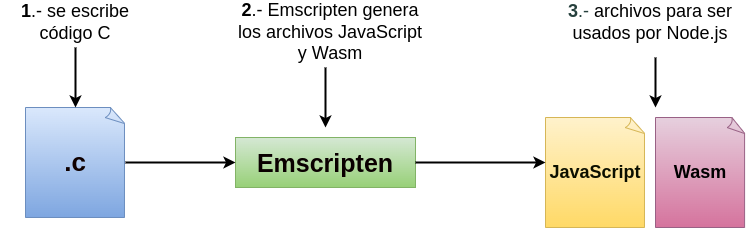
\includegraphics[scale=.47]{./Figures/Emscripten.png}
	\caption{Diagrama de funcionamiento de \textit{Emscripten}.}
	\label{fig:Emscripten}
\end{figure}


En ese sentido, para la aplicación de usuario dentro de la plataforma, cuando se ejecuta un programa de usuario, \textit{Emscripten} utiliza una función del módulo de \textit{Node.js} para la generación de un identificador único que será utilizado para los archivos generados. Este identificador esta compuesto por el prefijo \texttt{user\_} y un número entero que representa el tiempo en milisegundos. Es decir, \textit{Emscripten} creará los siguientes archivos:

\begin{itemize}

	\item Archivo \texttt{user\_tiempoenmilisegundos.js}: resultado final de la compilación y contiene el código \textit{JavaScript} que representa el programa \textit{C}.
	\item Archivo \texttt{user\_tiempoenmilisegundos.wasm}: contiene el código binario equivalente al código \textit{C} compilado. Se utiliza si el navegador del usuario admite \textit{WebAssembly} y proporciona un rendimiento mejorado en comparación con el código \textit{JavaScript} puro.
	\item Archivo \texttt{user\_tiempoenmilisegundos.js.components}: contiene datos utilizados por el programa.
	\item Archivo \texttt{user\_tiempoenmilisegundos.wasm.map}: contiene rutas de mapeos a los archivos de código \textit{C} que fueron compilados en formato \textit{Json}.
	\item Archivo \texttt{user\_tiempoenmilisegundos.wast}: representa el módulo \textit{WebAssembly} generado, pero en una representación de texto legible.
\end{itemize}

Estos archivos se ubicarán dentro del directorio de salida  \textit{outUser} que fue previamente configurado.


\subsection{JavaScript HAL}

Esta capa de programación se diseñó para proporcionar la funcionalidad de distribuir los eventos entre los componentes de la interfaz de usuario de \textit{JavaScript} y la capa \textit{C HAL}. Para lograr este objetivo se usaron las clases \textit{EventEmitter} del módulo \textit{Events} que monitorizan y activan los eventos. Además, facilita la interacción del navegador con el código \textit{JavaScript} y la actualización de la interfaz de usuario de manera flexible y eficiente.

También, la clase \textit{EventEmitter} se basa en el modelo de publicación/suscripción que se trata de un paradigma de envío de mensajes asíncrono mediante el cual un usuario publica mensajes y uno o varios objetos se suscriben a esos eventos.

En la figura \ref{fig:PublicarSuscribir} se muestra el modelo de \textit{publicación/suscripción}.

\begin{figure}[ht]
	\centering
	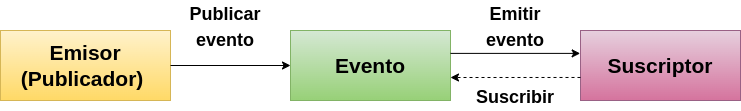
\includegraphics[scale=.49]{./Figures/PublicarSuscribir.png}
	\caption{Modelo de \textit{publicación/suscripción}.}
	\label{fig:PublicarSuscribir}
\end{figure}


Para la implementacion de esta capa de emulación, se crearon archivos \textit{JavaScript} con instancias de la clase \textit{EventEmitter}, que al utilizar el método \textit{emit} lanzan eventos con nombre. El nombre del evento es un string y permite que los oyentes registrados al evento sean notificados. La figura \ref{fig:EventemitterNodejs} muestra el diagrama de bloques de la instancia de \textit{EventEmitter} en la plataforma de emulación.

\begin{figure}[ht]
	\centering
	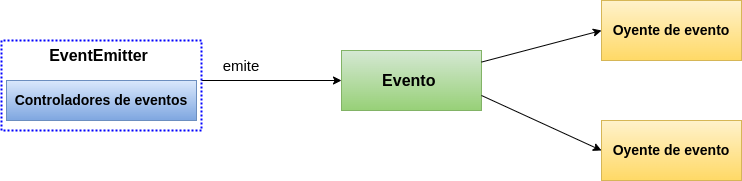
\includegraphics[scale=.49]{./Figures/EventemitterNodejs.png}
	\caption{Diagrama de bloques de \textit{EventEmitter} implementado en la plataforma.}
	\label{fig:EventemitterNodejs}
\end{figure}

En la sección de \ref{sec:caso_de_estudio}, se mostrará la implementación de este modelo en los archivos \textit{JavaScript} del emulador web.

\subsection{\textit{\textbf{sapi\_gpio}}}

Para comenzar a emular la biblioteca \textit{sapi\_gpio} del proyecto CIAA, se identificaron las funciones principales que el entorno de la plataforma web debería ofrecer al usuario. La siguiente tabla \ref{tab:sapiGPIO} muestra las funciones del archivo de código fuente \textit{sapi\_gpio} en la biblioteca \textit{\textbf{sAPI}} del proyecto CIAA que también están presentes en el emulador.


\begin{table}[h]
	\centering
	\caption[Funciones \texttt{sapi\_gpio}]{Funciones \texttt{sapi\_gpio}}
	\begin{tabular}{p{0.20\linewidth} p{0.50\linewidth}  p{0.20\linewidth}}    
		\toprule
		\textbf{Función} 	 & \textbf{Parámetros} 		& \textbf{Tipo de retorno}  \\
		\midrule
		gpioInit & gpioMap\_t pin, gpioInit\_t config 		&  bool\_t \\		
		gpioRead	 & gpioMap\_t pin			&  bool\_t \\
		gpioWrite	 & gpioMap\_t pin, bool\_t value			& bool\_t \\
		gpioToggle	 & gpioMap\_t pin				&  bool\_t \\
		\bottomrule
		\hline
	\end{tabular}
	\label{tab:sapiGPIO}
\end{table}

Además, para lograr replicar el comportamiento de cada función emulada de manera que, al invocarlas, produzcan resultados similares a los que se obtendrían al utilizar las funciones con el hardware físico, se utilizó la capa de \textit{C HAL}. Esta capa interactúa con la capa \textit{Javascript HAL}, que se encarga de comunicarse con la interfaz de usuario, permitiendo mostrar el comportamiento de los pines GPIO programados en la aplicación del usuario.

Entonces, se utilizó la capa de emulación correspondiente a \textit{C HAL} para emular las siguientes funcionalidades:

\begin{itemize}
	\item \texttt{Chip\_GPIO\_Init(LPC\_GPIO\_PORT)}se utiliza para inicializar y configurar el hardware de los pines GPIO de la placa. En la capa de emulación \textit{C HAL}, utilizando  \textit{Emscripten}, también se realizaron configuraciones de variables para representar los tipos de pines e inicializarlos.
	
	\item \texttt{Chip\_GPIO\_SetDir (LPC\_GPIO\_PORT, gpioPort, \newline (1 \<<\<<  gpioPin), GPIO\_OUTPUT)}se utiliza para establecer si un pin GPIO se utilizará para recibir datos (entrada) o enviar datos (salida). De manera similar, en la capa de abstracción de datos en \textit{C}, se implementaron configuraciones similares para la capa \textit{Javascript HAL} usando las macros de \textit{Emscripten}.
	
	\item \texttt{Chip\_GPIO\_SetPinState(LPC\_GPIO\_PORT, gpioPort, \newline gpioPin, 0)} se utiliza para gestionar el estado de los pines GPIO, permitiendo configurarlos como salidas y establecer su valor (alto o bajo). En la capa de abstracción de datos \textit{C}, esta función actualiza la estructura de datos utilizada para almacenar información sobre la configuración de los pines GPIO. Además, registra el valor del pin especificado como parámetro.

	\item \texttt{Chip\_GPIO\_ReadPortBit(LPC\_GPIO\_PORT, gpioPort, \newline gpioPin)} se utiliza para obtener el estado actual de un pin GPIO específico en la placa, lo que permite leer datos provenientes de dispositivos externos o de otros componentes conectados a los pines GPIO. En la capa de emulación \textit{C HAL}, se emula la lectura del estado de un pin GPIO utilizando la información almacenada en la estructura de datos.
\end{itemize}


Para emular las funciones mencionadas anteriormente, se utilizó la macro \newline \texttt{EM\_ASM\_}, mediante la cual se incrustó código \textit{JavaScript} directamente en el código \textit{C}. Este código \textit{JavaScript} incrustado se compila junto con el código C y se ejecutará en el entorno de ejecución de \textit{Emscripten}  cuando la aplicación de usuario invoque a esas funciones. La figura \ref{fig:gpioEmscripten} muestra el diagrama de bloques de la macro \texttt{EM\_ASM\_}.

\hfill \break


\begin{figure}[ht]
	\centering
	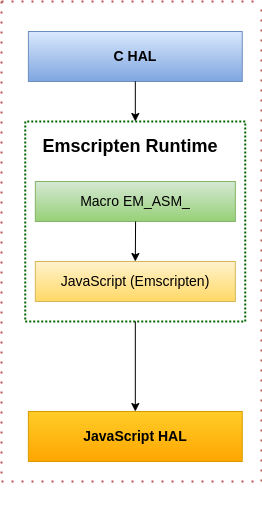
\includegraphics[scale=.40]{./Figures/gpioEmscripten.png}
	\caption{Diagrama de bloques de la macro \texttt{EM\_ASM\_}.}
	\label{fig:gpioEmscripten}
\end{figure}


Asimismo, para emular las interacciones entre la interfaz de usuario y las GPIO TEC1, TEC2, TEC3 y TEC4, se utilizó en la capa \textit{C HAL} la macro \newline \texttt{EMSCRIPTEN\_KEEPALIVE}. Su funcionamiento se explica en la siguiente sección \ref{sec:sapi_tick}. 

A continuación, en la capa \textit{Javascript HAL}, se distribuyen eventos a la capa \textit{Javascript UI} para notificarle que el pin GPIO ha sido configurado desde la capa \textit{C HAL}. Estos eventos incluyen información que será útil para gestionar los pines GPIO en la capa de interfaz de usuario. La figura \ref{fig:gpioEmit} muestra el diagrama de bloques del envío de eventos de la capa \textit{Javascript HAL} a la capa \textit{Javascript UI}.

\begin{figure}[ht]
	\centering
	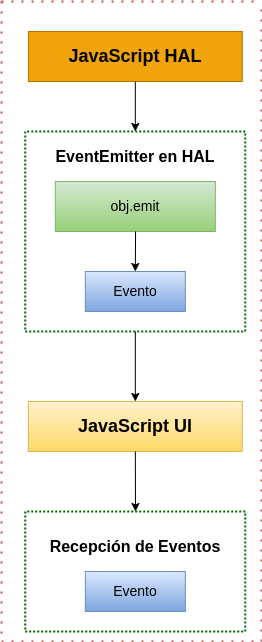
\includegraphics[scale=.40]{./Figures/gpioEmit.png}
	\caption{Diagrama de bloques del envío de eventos de la capa \textit{Javascript HAL}.}
	\label{fig:gpioEmit}
\end{figure}

Por consiguiente, en la capa \textit{Javascript UI} se manipulan esos eventos, y en consecuencia, se actualiza la interfaz de la plataforma web para mostrar al usuario los cambios.

\subsection{\textit{\textbf{sapi\_tick}}}
\label{sec:sapi_tick}

En la tabla \ref{tab:sapiTick} se puede observar las funciones del archivo de código fuente \texttt{sapi\_tick} en la biblioteca \textit{\textbf{sAPI}} del proyecto CIAA y en el emulador.

\begin{table}[h]
	\centering
	\caption[Funciones \texttt{sapi\_tick}]{Funciones \texttt{sapi\_tick}}
	\begin{tabular}{p{0.20\linewidth} p{0.50\linewidth}  p{0.20\linewidth}}    
		\toprule
		\textbf{Función} 	 & \textbf{Parámetros} 		& \textbf{Tipo de retorno}  \\
		\midrule
		tickInit & tick\_t tickRateMSvalue 		&  bool\_t \\		
		tickRead	 & void				&  tick\_t \\
		tickWrite	 & tick\_t ticks 				& void \\
		tickCallbackSet	 & callBackFuncPtr\_t tickCallback, void* tickCallbackParams				&  bool\_t \\
		tickPowerSet & bool\_t power 		&  void \\	
		\bottomrule
		\hline
	\end{tabular}
	\label{tab:sapiTick}
\end{table}

Para emular a nivel de API, se tuvo como objetivo replicar el comportamiento de la función \texttt{tickInit}, la cual se encarga de la inicialización y configuración de la interrupción del temporizador \texttt{SysTick\_Config} en la placa física. Sin embargo, al realizar la emulación en la plataforma web, esta función no se encuentra disponible de forma nativa. Por lo tanto, fue necesario emular su comportamiento y proporcionar una alternativa compatible.

Para emular la funcionalidad de \texttt{SysTick\_Config}, se utilizó la capa de emulación correspondiente a \textit{C HAL}. Esta capa de emulación permitió ejecutar código \textit{JavaScript} en el contexto de \textit{Emscripten}, lo que posibilitó replicar el comportamiento del temporizador \textit{SysTick}. 

Una vez habilitada la interrupción del temporizador, se realiza una invocación periódica a la función \texttt{tickerCallback}, que tiene la misma implementación que en \texttt{sapi\_tick} de la biblioteca \textit{\textbf{sAPI}} del proyecto CIAA. La función \newline \texttt{tickerCallback} realiza las siguientes acciones: incrementa los contadores de ticks y, si el puntero \texttt{tickHookFunction} no es nulo, ejecuta la función establecida como \textit{calback} mediante la función de \textit{\textbf{sAPI}} \texttt{tickCallbackSet()}, pasando los parámetros \texttt{callBackFuncParams}. En consecuencia, esto permite la ejecución de tareas específicas programadas por el usuario en cada interrupción del temporizador periódico.

En el capítulo 4 se detallarán las diferencias encontradas al realizar las pruebas entre la placa y el emulador utilizando estas funciones.

En el contexto de la emulación a nivel de API, para implementar las demás bibliotecas de las \textit{\textbf{sAPI}}, se siguió el mismo esquema utilizado en \texttt{sapi\_tick}. Primeramente, se identificaron las funciones que requerían interacción con el hardware de la placa. Luego, en la capa \textit{C HAL} se implementaron funciones de emulación con \textit{Emscripten} para reflejar el comportamiento del hardware.

Para emular el comportamiento de la interrupción del temporizador \textit{SysTick} y proporcionar la invocación periódica a la función \texttt{tickerCallback} de \textit{sapi\_tick}, se utilizó la macro \texttt{EMSCRIPTEN\_KEEPALIVE} de \textit{Emscripten}, que le dice al compilador de \textit{Emscripten} que conserve la función marcada con esta macro en el código compilado, incluso si no es accedida desde el código \textit{JavaScript} del lado del cliente.

Es decir, cuando la función marcada con la macro \texttt{EMSCRIPTEN\_KEEPALIVE} sea invocada desde la capa \textit{JavaScript HAL}, llamará a la función \texttt{tickerCallback} de la biblioteca \textit{C} y la ejecutará. En la figura \ref{fig:tickerCallback} se muestra el funcionamiento de \texttt{EMSCRIPTEN\_KEEPALIVE}. 


\begin{figure}[ht]
	\centering
	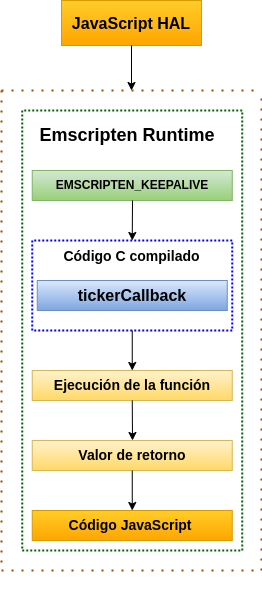
\includegraphics[scale=.55]{./Figures/tickerCallback.png}
	\caption{Diagrama de bloques \texttt{EMSCRIPTEN\_KEEPALIVE}.}
	\label{fig:tickerCallback}
\end{figure}



Para lograr la interacción con la capa de emulación \textit{C HAL}, y realizar la invocación periódica a la función que usa la macro \texttt{EMSCRIPTEN\_KEEPALIVE} de \textit{Emscripten} se configuró en esta capa de desarrollo un temporizador de \textit{JavaScript}.

Además, dentro del temporizador, se utilizó la función \texttt{ccall} de \textit{Emscripten}, que permite invocar a la funcion \texttt{tickerCallback} desde el código \textit{C} compilado con \textit{Emscripten}. 

A continuacion, se muestra en la figura  \ref{fig:ccall} el funcionamiento de \texttt{ccall}. 

\hfill \break
\hfill \break
\hfill \break
\hfill \break

\begin{figure}[ht]
	\centering
	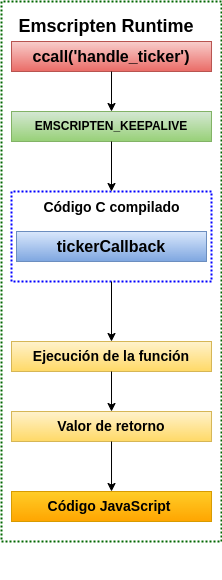
\includegraphics[scale=.49]{./Figures/ccall.png}
	\caption{Diagrama de bloques de la función \textit{ccall}.}
	\label{fig:ccall}
\end{figure}

Sin embargo, debido a la naturaleza asíncrona de \textit{JavaScript} y al uso de la función \texttt{ccall}, la función no mantiene el contexto entre las ejecuciones del temporizador. En consecuencia, cada vez que se reinicia el temporizador y se ejecuta la función  \texttt{tickerCallback}, la tarea específica programada por el usuario comienza desde el principio en lugar de continuar desde el punto donde quedó anteriormente. 

\subsection{\textit{\textbf{sapi\_delay}}}

La tabla \ref{tab:sapiDelay} expone las funciones del archivo de código fuente \texttt{sapi\_delay} en la biblioteca \textit{\textbf{sAPI}} del proyecto CIAA y en el emulador.

\begin{table}[h]
	\centering
	\caption[Funciones \texttt{sapi\_delay}]{Funciones \texttt{sapi\_delay}}
	\begin{tabular}{p{0.30\linewidth} p{0.40\linewidth}  p{0.20\linewidth}}    
		\toprule
		\textbf{Función} 	 & \textbf{Parámetros} 		& \textbf{Tipo de retorno}  \\
		\midrule
		delayInaccurateMs & tick\_t delay\_ms 		&  void \\		
		delayInaccurateUs	 & tick\_t delay\_us			&  void \\
		delayInaccurateNs	 & tick\_t delay\_ns				& void \\
		delay	 & tick\_t duration\_ms				&  void \\
		delayInit & delay\_t * delay, tick\_t duration 		&  void \\
		delayRead & delay\_t * delay 		&  bool\_t \\
		delayWrite & delay\_t * delay, tick\_t duration 		&  void \\	
		\bottomrule
		\hline
	\end{tabular}
	\label{tab:sapiDelay}
\end{table}

La función \texttt{delay} en la biblioteca \textit{\textbf{sAPI}} del proyecto CIAA crea una pausa en la ejecución del programa durante el tiempo especificado en \texttt{duration\_ms} implementando un bucle de espera. Este bucle se ejecutará mientras la diferencia de tiempo entre \texttt{tickRead()} y startTime(inicio actual de \texttt{tickRead()} sea menor que \texttt{duration\_ms/ tickRateMS}.

Sin embargo, cuando \textit{Emscripten} compila código \textit{C} a \textit{JavaScript}, la función \texttt{delay} tal como está escrita, causa que la ejecución de la plataforma web se bloquee o congele. Esto se debe a que la función \texttt{tickRead()} no se actualiza a la velocidad que se espera, lo que lleva a que se obtenga el mismo valor repetidamente. Es decir, debido a la naturaleza asincrónica de \textit{JavaScript} y al no tener una pausa controlada en el bucle (como \texttt{delay(1)}), \textit{JavaScript} no tiene tiempo suficiente para actualizar el valor de \texttt{tickRead()} entre iteraciones. De esta manera,  el bucle \texttt{while} se queda esperando activamente e impide al navegador atender otros eventos.

Por esta razón, se decidio usar en las funciones de espera,  las funciones nativas de \textit{Emscripten} usando la capa de emulación \textit{C HAL}, que se ira detallando en la siguiente sección. En consecuencia, se aprovecho su eficiencia y precisión.

Para emular las funciones de espera de la biblioteca \textit{C} se implemento la función \texttt{emscripten\_sleep}, que utiliza funciones asincrónicas internas de \textit{Emscripten} para realizar pausas. 

Por lo tanto, permite al navegador atender otros eventos mientras el programa se encuentra en espera. Es decir, evita el bloqueo de la ejecución del resto del código y también, que la página no responda.

Además, proporciona pausas precisas, debido a que, \textit{Emscripten}  utiliza las capacidades de temporización del navegador para garantizar que el tiempo indicado sea realizado.

La figura \ref{fig:emscriptenDelay} representa el funcionamiento de  \texttt{emscripten\_sleep}. 


\begin{figure}[ht]
	\centering
	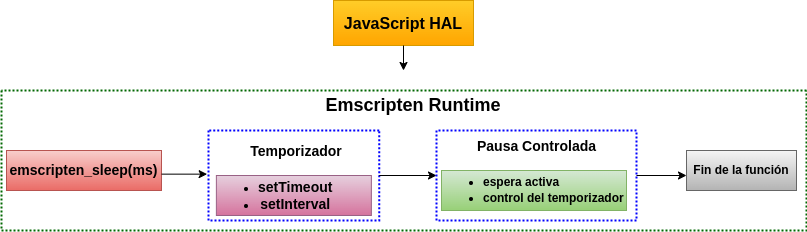
\includegraphics[scale=.50]{./Figures/emscriptenDelay.png}
	\caption{Diagrama de bloques \texttt{emscripten\_sleep.}}
	\label{fig:emscriptenDelay}
\end{figure}




\subsection{\textit{\textbf{freertos}}}

Para emular la funcionalidad de las tareas de \textit{freeRTOS} en el contexto del emulador web, se utilizó la biblioteca de eventos de \textit{mbed}. Entonces, para las funciones \texttt{xTaskCreate} y \texttt{xTaskCreateStatic}, se programaron funciones periódicas utilizando las siguientes funciones de la biblioteca de \textit{Mbed events}: 

 
 \begin{itemize}
	\item \texttt{int equeue\_create}:  crea una cola de eventos, configura e inicializa los recursos de plataforma necesarios, como semáforos y mutexes.
	
	\item \texttt{int equeue\_call\_every}:  se utiliza para crear un evento periódico en la cola de eventos equeue, programando llamadas repetidas a una función en intervalos regulares.
	
	\item \texttt{int equeue\_post}: permite publicar un evento en la cola de eventos equeue, estableciendo el tiempo y estableciendo el evento en la cola para su posterior procesamiento.
	
	\item \texttt{void equeue\_dispatch}: se encarga de despachar los eventos en la cola de eventos equeue de manera continua, verificando los tiempo y realizando acciones específicas según la configuración.

	\item \texttt{void equeue\_destroy}: permite liberar y limpiar todos los recursos asociados a una cola de eventos, libera los mutexes, semáforos y memoria asignada.
\end{itemize}

Estas funciones permiten ejecutar tareas periódicas en intervalos de tiempo regulares, lo que proporcionó una aproximación simplificada a la funcionalidad de tareas en el emulador web. Aunque esta solución no ofrece todas las características de un sistema operativo de tiempo real completo como \textit{freeRTOS}, fue adecuada para emular el funcionamiento de programas de usuario simples.

Es importante destacar que la implementación de tareas en el emulador web tiene una limitación significativa. Debido a que solo puede ejecutar un subproceso (hilo de ejecución) a la vez, no es posible que se ejecuten tareas simultáneas. Esto significa que, a diferencia del sistema operativo de tiempo real \textit{freeRTOS}, donde se pueden crear múltiples tareas que se ejecutan de manera concurrente, en el emulador web solo es posible ejecutar una sola tarea. Por lo tanto, esta solución es adecuada para programas de usuario simples que no requieran multitarea.


La tabla \ref{tab:ConceptosRTOS} expone algunos de los conceptos importantes de \textit{freeRTOS} que se cumplen en el emulador.

\begin{table}[h]
\centering
\caption[Conceptos importantes de \textit{freeRTOS} que se cumplen en el emulador.]{Conceptos importantes de \textit{freeRTOS} que se cumplen en el emulador.}
\begin{tabular}{p{0.45\linewidth} p{0.15\linewidth}  p{0.15\linewidth}}
\toprule
\textbf{Capacidades} 
& \textbf{\textit{freeRTOS}}
& \textbf{Emulador}
\\
\midrule
Multitareas & Si & No  \\
Funciones de espera &  Si & Si \\
Cambio de contexto &  Si & Si \\
Tarea de procesamiento continuo &  Si & Si \\
Manejo de prioridades & Si & No  \\
\bottomrule
\hline
\end{tabular}
\label{tab:ConceptosRTOS}
\end{table}

En el emulador, se encuentran implementados varios conceptos importantes de \textit{freeRTOS}, como funciones de espera y cambio de contexto. Sin embargo, en esta primera versión del emulador, no se han incluido el manejo de multitareas y de prioridades presentes en \textit{freeRTOS}.


\subsection{\textit{\textbf{sapi\_dht11}}}

Al emular los periféricos externos de la biblioteca \textit{\textbf{sAPI}} del proyecto CIAA, se continuó con la misma lógica de programación utilizada para interactuar con los periféricos de la placa EDU-CIAA-NXP. Asimismo, se mapearon las funcionalidades ofrecidas por la biblioteca \textit{\textbf{sAPI}} a la plataforma web. En la siguiente tabla \ref{tab:sapiDht11} se muestran las funciones presentes en ambas plataformas.


\begin{table}[h]
	\centering
	\caption[Funciones \texttt{sapi\_dht11}]{Funciones \texttt{sapi\_dht11}}
	\begin{tabular}{p{0.20\linewidth} p{0.50\linewidth}  p{0.20\linewidth}}    
		\toprule
		\textbf{Función} 	 & \textbf{Parámetros} 		& \textbf{Tipo de retorno}  \\
		\midrule
		dht11Init & int32\_t gpio		&  void \\		
		dht11Read	 & float *phum, float *ptemp	&  bool\_t \\
		\bottomrule
		\hline
	\end{tabular}
	\label{tab:sapiDht11}
\end{table}

En esta primera versión de la plataforma web, no se ofrece la capacidad gráfica de las interacciones virtuales entre la placa y los periféricos externos. Sin embargo, el usuario debe realizar las configuraciones manualmente, eligiendo las conexiones correctas, que luego serán verificadas en la capa de \textit{JavaScript UI}.
Además, en \textit{JavaScript UI}, principalmente se centró el trabajo de emular el envío de los datos de temperatura y humedad del sensor DHT11 al microcontrolador.


Entonces, en la capa de abstracción de datos \textit{C HAL} se implementó la lectura de los datos provenientes de la capa \textit{JavaScript HAL} al usar la macro \texttt{EM\_ASM\_INT} de \textit{Emscripten}. A continuación, en la figura \ref{fig:dht11Emscripten} se presenta el diagrama de bloques de la macro \texttt{EM\_ASM\_INT}.

\begin{figure}[ht]
	\centering
	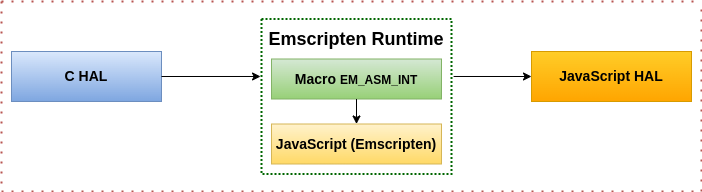
\includegraphics[scale=.53]{./Figures/dht11Emscripten.png}
	\caption{Diagrama de bloques de la macro \texttt{EM\_ASM\_INT}.}
	\label{fig:dht11Emscripten}
\end{figure}

La capa \textit{JavaScript HAL} recibe los datos enviados desde \textit{JavaScript UI} y los transmite a la capa \textit{C HAL}. La generación de los datos  emulados de temperatura y humedad, se realiza en \textit{JavaScript UI} a través de dos opciones elegidas por el usuario:
 
 \begin{itemize}
	\item Obtener los datos de temperatura y humedad local conectándose a una central meteorológica a través de la geolocalización del navegador del usuario. Sin embargo, si el servidor donde se encuentra desplegada la plataforma web no puede acceder al servicio de geolocalización del navegador por motivos de seguridad, o el usuario no permite el acceso, entonces se realizará la consulta a la central meteorológica utilizando la ubicación predeterminada de la ciudad de Buenos Aires. Acto seguido se actualizará la interfaz gráfica con los datos de temperatura y humedad.
	
	\item Generar los datos manualmente haciendo click en la interfaz gráfica que representa a la temperatura y humedad. De esta manera, el usuario puede generar los datos según su elección.
\end{itemize}

En la figura \ref{fig:uiDht11} se muestra el diagrama de bloques de la capa de interfaz de usuario \textit{JavaScript UI} con las dos opciones de usuario.

\begin{figure}[ht]
	\centering
	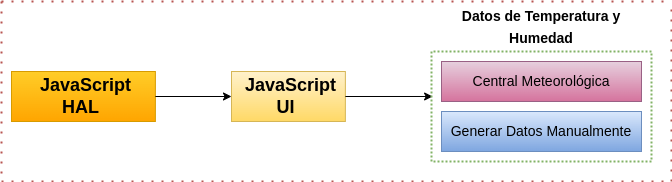
\includegraphics[scale=.53]{./Figures/uiDht11.png}
	\caption{Diagrama de bloques de la capa \textit{JavaScript UI} con las dos opciones para el usuario.}
	\label{fig:uiDht11}
\end{figure}

\hfill \break
\hfill \break
\hfill \break
\hfill \break

\subsection{\textit{\textbf{sapi\_adc}}}

Para comenzar, se realizó el mapeo de las funciones del módulo de la biblioteca \textit{\textbf{sAPI}} a la plataforma web. La tabla \ref{tab:sapiADC} expone las funciones presentes en ambas plataformas.


\begin{table}[h]
	\centering
	\caption[Funciones \texttt{sapi\_adc}]{Funciones \texttt{sapi\_adc}}
	\begin{tabular}{p{0.20\linewidth} p{0.50\linewidth}  p{0.20\linewidth}}    
		\toprule
		\textbf{Función} 	 & \textbf{Parámetros} 		& \textbf{Tipo de retorno}  \\
		\midrule
		adcInit & adcInit\_t config		&  void \\		
		adcRead	 & adcMap\_t analogInput	&  uint16\_t \\
		\bottomrule
		\hline
	\end{tabular}
	\label{tab:sapiADC}
\end{table}

El módulo \textit{adc} fue implementado en el emulador  y es utilizado por varios periféricos externos, que incluyen: el potenciómetro, el termistor NTC y el joystick. De esta manera, permite al usuario realizar pruebas de funcionamiento de un \textit{adc} real. 

Luego, se implementaron las funciones de inicialización y de lectura del componente \textit{adc}  en la capa \textit{C HAL}. Posteriormente, son utilizadas por la capa \textit{JavaScript HAL} para la interacción con el hardware y permitir al usuario trabajar con los periféricos externos en un entorno web. La figura \ref{fig:adcEmscripten} presenta el diagrama de bloques de las capas: \textit{C HAL} y \textit{JavaScript HAL} para el \textit{adc}.

\begin{figure}[ht]
	\centering
	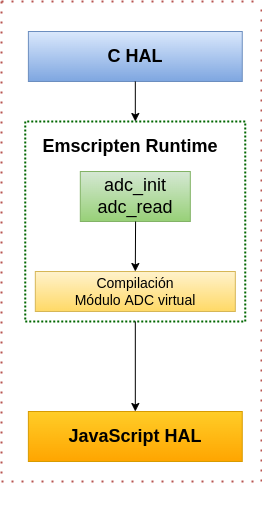
\includegraphics[scale=.53]{./Figures/adcEmscripten.png}
	\caption{Diagrama de bloques de \textit{C HAL} y \textit{JavaScript HAL} para el módulo \textit{adc}.}
	\label{fig:adcEmscripten}
\end{figure}

\hfill \break
\hfill \break
\hfill \break
\hfill \break

En la capa \textit{JavaScript UI}, se implementó la obtención de datos para los periféricos externos que interactúan con el \textit{adc}. Por ejemplo, para el potenciómetro, los datos son establecidos por el usuario a través de la interfaz gráfica utilizando el componente HTML  \textit{input} de tipo \textit{range}. De esta manera, el usuario al deslizar este componente dentro de un rango mínimo y máximo establecido, se va realizando el siguiente cálculo para obtener el valor del \textit{adc} correspondiente:

\begin{lstlisting}[caption={Cálculo del ADC para el potenciómetro.}]
  window.JSHal.gpio.write(self.dataPin.ADC, range.value/ 3.3 * 1023);
\end{lstlisting}

En consecuencia, los cálculos actualizados se muestran en la interfaz gráfica del emulador web.

En el caso del termistor NTC, se implementó en la interfaz grafica un elemento gráfico (termómetro) para representar la temperatura en grados celsius. A medida que el usuario ajusta el termómetro, la temperatura en kelvin se va actualizando en función de la temperatura en grados celsius y, además, el valor del \textit{adc} se actualiza mediante la siguiente función:

\begin{lstlisting}[caption={Cálculo ADC del termistor NTC.}]
     ThermistorNTC.prototype.updateSampleADC= function(R_NTC) {
        let R_NTC_float = parseFloat(R_NTC);
        let R_10k_float = parseFloat(R_10k);
        let Vsupply_float = parseFloat(Vsupply);    
        let VoutT = (R_NTC_float * Vsupply_float) / (R_10k_float + R_NTC_float);
        Vout = parseFloat(VoutT.toFixed(2)); 

        this.sample = parseFloat((Vout * 1023.0 / Vsupply).toPrecision(4));
        console.log('this.sample ', this.sample);
        window.JSHal.gpio.write(this.dataPin.ADC, this.sample);     
    };
\end{lstlisting}

Además, se implementó un componente web para el joystick, encargado de gestionar los movimientos y acciones en las interacciones con el usuario. Los datos de los movimientos de los ejes X e Y del joystick son obtenidos y se utilizan para realizar cálculos de voltajes en las respectivas resistencias de cada eje, así como también, para calcular el valor del \textit{adc}. A modo de referencia se muestra las cálculos que se hicieron para el eje X del joystick:

\begin{lstlisting}[caption={Cálculo de la resistencia del eje X y del ADC.}]
            var VRx = Joy.GetVRx();
            var voltage = (Math.floor(VRx/ 3.3 * 1023)* 3.3 / 1023.0).toFixed(2);
            joyVRx.textContent = voltage;
            joyADCx.textContent = Math.trunc(VRx/ 3.3 * 1023);
            window.JSHal.gpio.write(self.dataPin.ADCx, VRx/ 3.3 * 1023);
\end{lstlisting}

Luego, para cada periférico externo, el cálculo del \textit{adc} es envíado a la capa \textit{JavaScript HAL}.
En la figura \ref{fig:uiADC} se muestra el diagrama de bloques con la interaccion de ambas capas de desarrollo.

\hfill \break
\hfill \break
\hfill \break

\begin{figure}[ht]
	\centering
	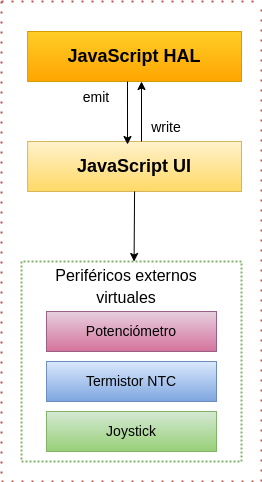
\includegraphics[scale=.57]{./Figures/uiADC.png}
	\caption{Diagrama de bloques con la interaccion de las capas  \textit{JavaScript HAL} y \textit{JavaScript UI}.}
	\label{fig:uiADC}
\end{figure}


\subsection{Tabla de Periféricos}

La siguiente tabla \ref{tab:perifericosInternosMBED} expone los  periféricos internos implementados actualmente en \textit{Mbed Simulator}.

\begin{table}[h]
\centering
\caption[Comparación de características de periféricos internos implementados en \textit{Mbed Simulator}]{Comparación de características de Periféricos internos implementados en \textit{Mbed Simulator}}
\begin{tabular}{p{0.24\linewidth} p{0.14\linewidth}  p{0.14\linewidth}  p{0.14\linewidth}}
\toprule
\textbf{Periféricos} 
& \textbf{Velocidad y tiempo real}
& \textbf{Responde a eventos}
\\
\midrule
GPIO & Si & Si  \\
UART & Si & Si \\
BUTTON & SI & Si \\
ADC & Si & Si \\
DAC & Si & No \\
PWM & Si & No \\ 
\bottomrule
\hline
\end{tabular}
\label{tab:perifericosInternosMBED}
\end{table}


En la figura \ref{fig:GPIOMbed} se muestra el funcionamiento de GPIO y en la figura \ref{fig:PMWMbed} expone el funcionamiento de PWM del \textit{Mbed Simulator}.

\hfill \break
\hfill \break
\hfill \break
\hfill \break
\hfill \break

\begin{figure}[ht]
	\centering
	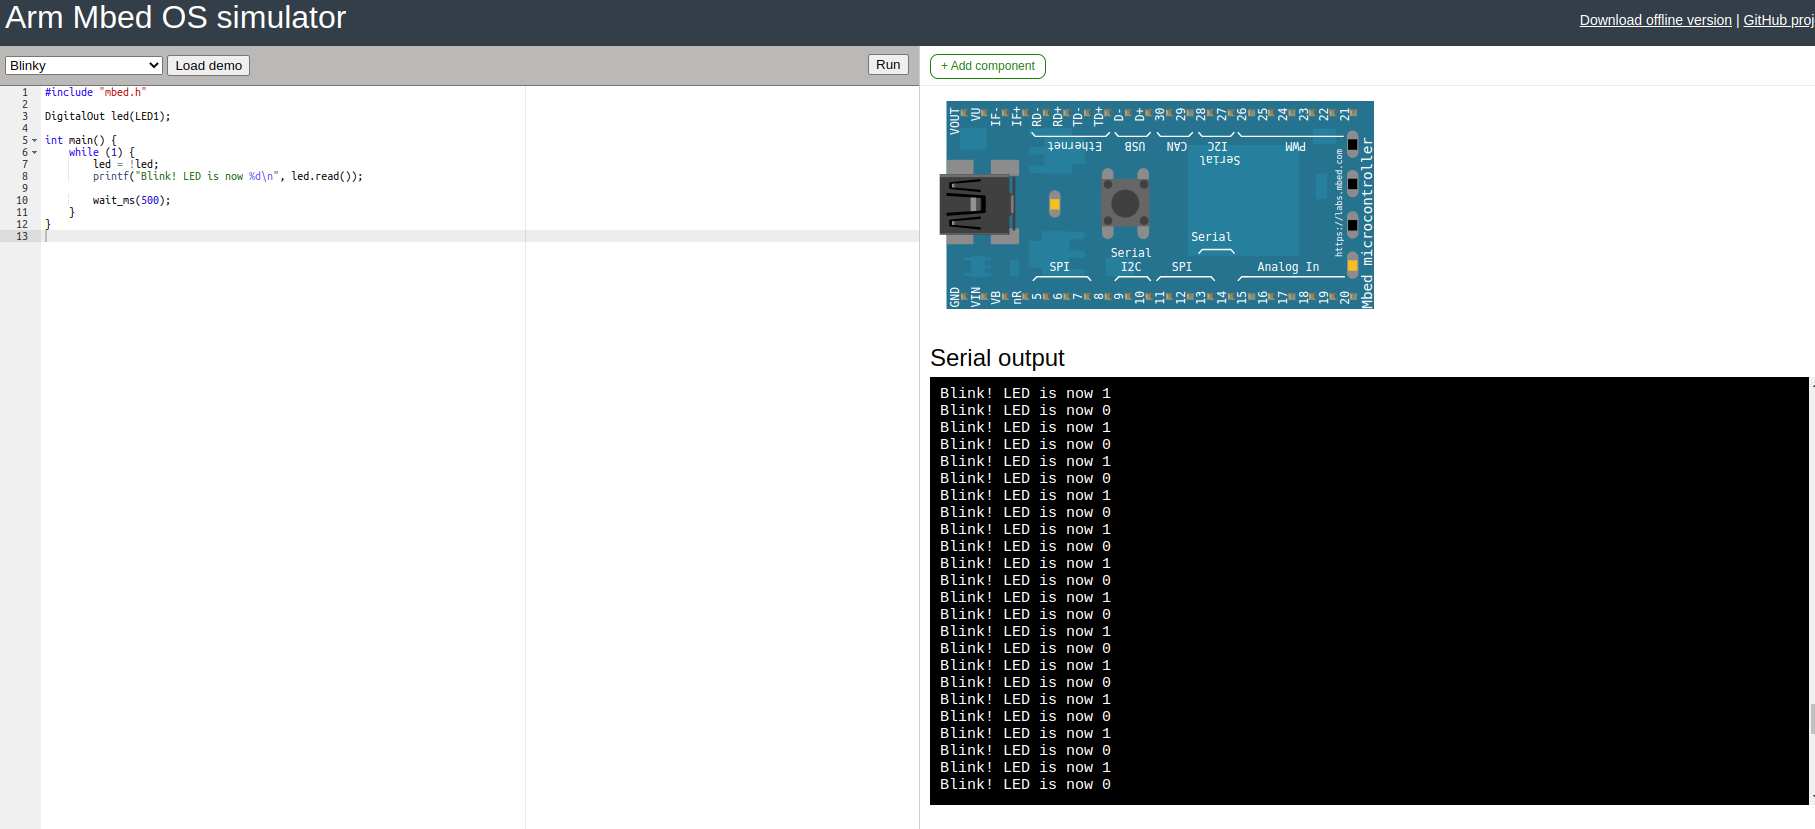
\includegraphics[scale=.24]{./Figures/GPIOMbed.png}
	\caption{Funcionamiento GPIO en \textit{Mbed Simulator}.}
	\label{fig:GPIOMbed}
\end{figure}

\begin{figure}[ht]
	\centering
	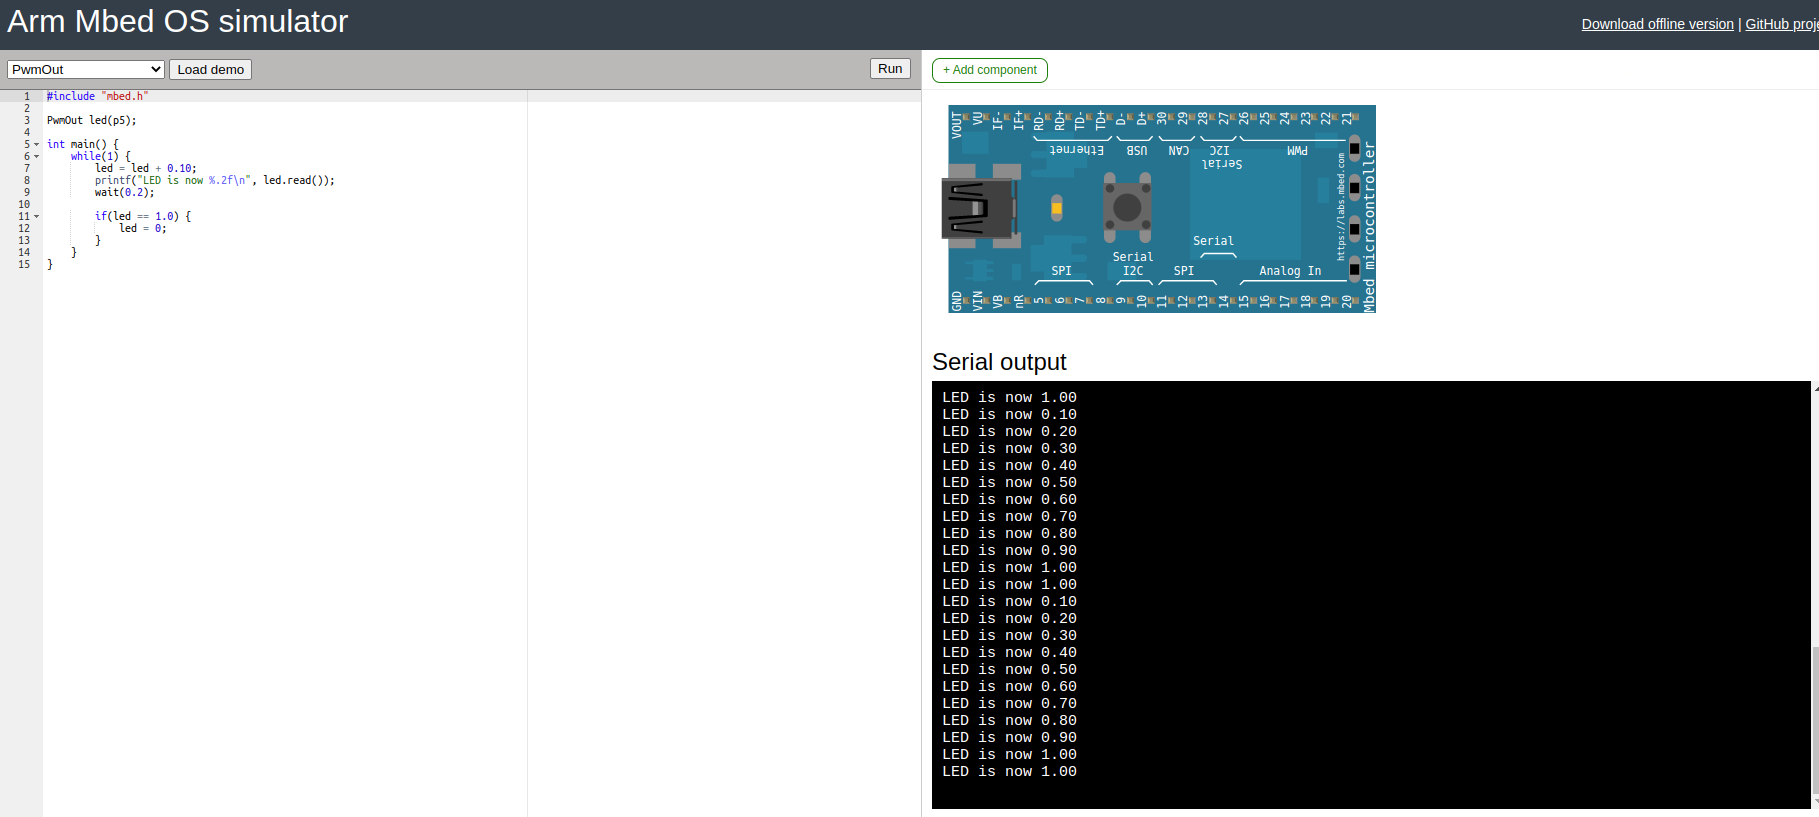
\includegraphics[scale=.24]{./Figures/PMWMbed.png}
	\caption{Funcionamiento PWM en \textit{Mbed Simulator}.}
	\label{fig:PMWMbed}
\end{figure}





Además, en la tabla \ref{tab:perifericosExternosMBED} expone los  periféricos externos implementados actualmente en \textit{Mbed Simulator}.


\begin{table}[h]
\centering
\caption[Comparación de características de Periféricos externos implementados en \textit{Mbed Simulator}]{Comparación de características de Periféricos externos implementados en \textit{Mbed Simulator}}
\begin{tabular}{p{0.30\linewidth} p{0.14\linewidth}  p{0.14\linewidth}  p{0.14\linewidth}}
\toprule
\textbf{Periféricos} 
& \textbf{Velocidad y tiempo real}
& \textbf{Responde a eventos}
\\
\midrule
DHT11 & Si & Si  \\
LCD Display C12832 & Si & Si  \\
LED & Si & Si \\
Thermistor & Si & Si \\
SHT31 & Si & Si \\
Touch Screen ST7789H2 & Si & Si \\
\bottomrule
\hline
\end{tabular}
\label{tab:perifericosExternosMBED}
\end{table}

La figura \ref{fig:perifericosMbed} muestra los periféricos externos de \textit{Mbed Simulator}.
\hfill \break
\hfill \break
\hfill \break
\hfill \break
\hfill \break

\begin{figure}[ht]
	\centering
	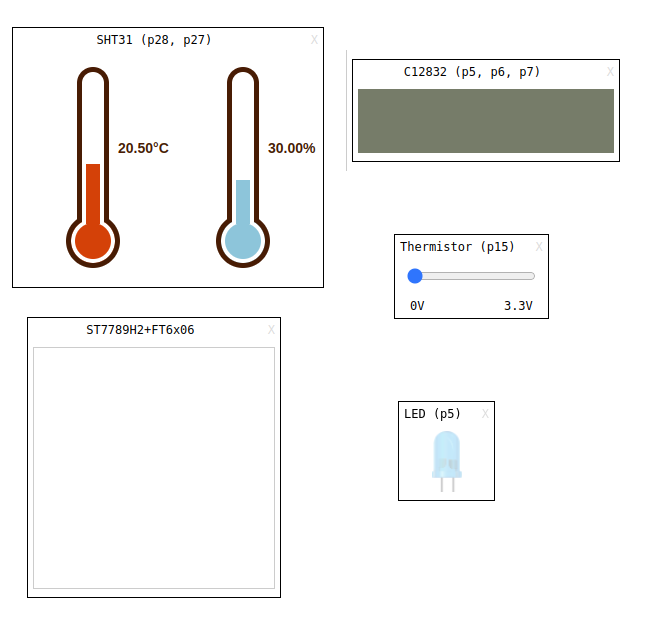
\includegraphics[scale=.81]{./Figures/perifericosMBED.png}
	\caption{Periféricos externos de \textit{Mbed Simulator}.}
	\label{fig:perifericosMbed}
\end{figure}

En la siguiente tabla \ref{tab:perifericosInternosCIAA} se exponen los  periféricos internos implementados en la primera versión de la plataforma de emulación web de la placa EDU-CIAA.

\begin{table}[h]
\centering
\caption[Comparación de características de periféricos internos del Emulador EDU-CIAA]{Comparación de características de Periféricos}
\begin{tabular}{p{0.24\linewidth} p{0.14\linewidth}  p{0.14\linewidth}  p{0.14\linewidth}}
\toprule
\textbf{Periféricos} 
& \textbf{Velocidad y tiempo real}
& \textbf{Responde a eventos}
\\
\midrule
GPIO & Si & Si  \\
UART & Si & Si \\
BUTTON & SI & Si \\
RTC & Si & Si  \\
SYSTICK & No & Si \\
ADC & Si & Si \\
DAC & Si & No \\
\bottomrule
\hline
\end{tabular}
\label{tab:perifericosInternosCIAA}
\end{table}


Además, la siguiente tabla \ref{tab:perifericosExternosCIAA} se exponen los  periféricos externos implementados en la plataforma de emulación web.

\hfill \break
\hfill \break
\hfill \break
\hfill \break

\begin{table}[h]
\centering
\caption[Comparación de características de periféricos externos del Emulador EDU-CIAA]{Comparación de características de los periféricos externos del Emulador EDU-CIAA}
\begin{tabular}{p{0.30\linewidth} p{0.14\linewidth}  p{0.14\linewidth}  p{0.14\linewidth}}
\toprule
\textbf{Periféricos} 
& \textbf{Velocidad y tiempo real}
& \textbf{Responde a eventos}
\\
\midrule
DHT11 & Si & Si  \\
LCD & Si & Si  \\
LED & Si & Si  \\
LCD DISPLAY 128x64 & Si & Si \\
LCD DISPLAY 20x4 & Si & Si \\
Thermistor NTC & Si & Si \\
Potentiometer & Si & Si \\
Joystick & Si & Si \\
\bottomrule
\hline
\end{tabular}
\label{tab:perifericosExternosCIAA}
\end{table}


La figura \ref{fig:perifericosCIAA} muestra los periféricos externos implementados en el emulador web EDU-CIAA.

\begin{figure}[ht]
	\centering
	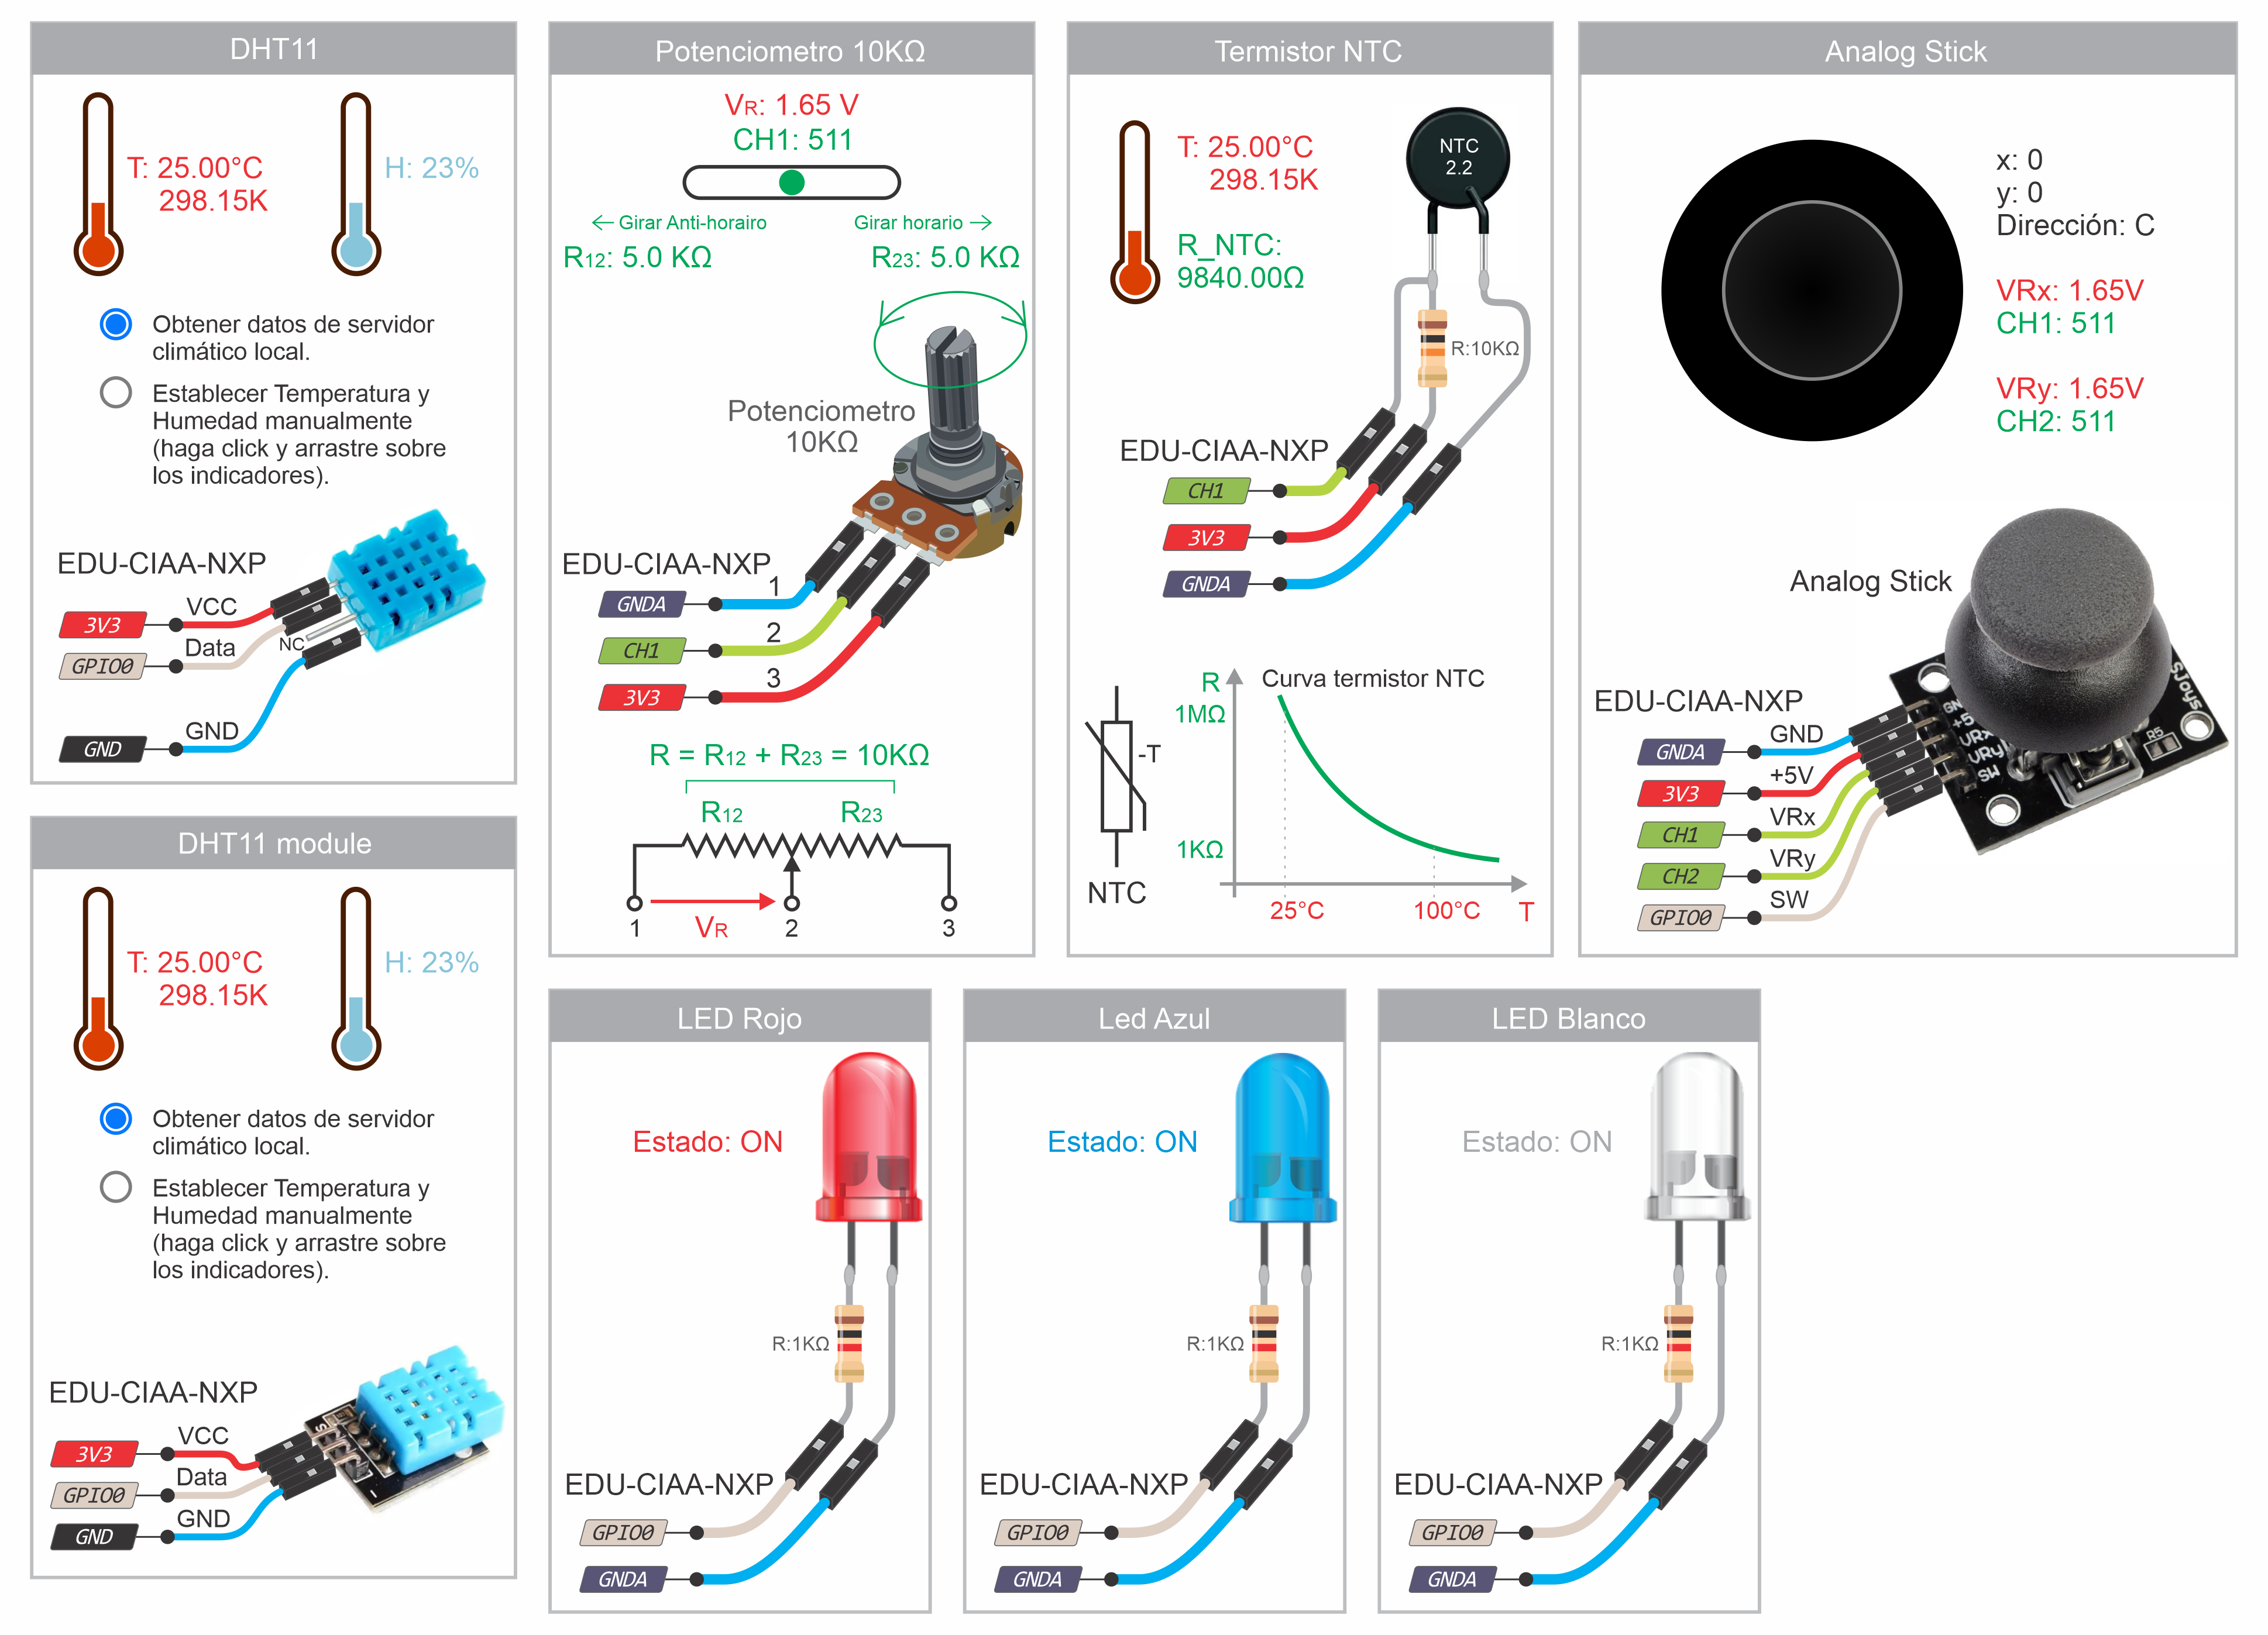
\includegraphics[scale=.40]{./Figures/perifericosCIAA.png}
	\caption{Periféricos externos del emulador web EDU-CIAA.}
	\label{fig:perifericosCIAA}
\end{figure}


\hfill \break
\hfill \break
\hfill \break
\hfill \break
\hfill \break
\hfill \break
\hfill \break
\hfill \break

\section{Caso de estudio}
\label{sec:caso_de_estudio}

El usuario escribe o modifica el programa llamado \texttt{blinky} en lenguaje \textit{C}, que utiliza la biblioteca \textit{\textbf{sAPI}} para interactuar con los periféricos de hardware GPIO y controlar el LED. A continuación, ejecuta el programa dentro de la plataforma web. Para lograr esto, Node.js se encarga de ejecutar los comandos necesarios para que \textit{Emscripten} realice la compilación del código \textit{C}, que incluye: 

\begin{itemize}
	\item El codigo de la aplicacion de usuario escrito en lenguaje \textit{C}.
	\item El archivo \texttt{sapi\_gpio.c} de la capa \textit{Bibioteca C}.
	\item El archivo \texttt{gpio\_api.c} de la capa \textit{C HAL}.
\end{itemize} 

El proceso de compilación comienza con el preprocesamiento del código \textit{C}, que incluye el manejo de directivas del preprocesador como \texttt{\#include} y \texttt{\#define}. Luego, el compilador utiliza \textit{LLVM} para compilar el código \textit{C} en \texttt{bitcode}. Después, de obtener el \texttt{bitcode} realiza optimizaciones para mejorar el rendimiento y reducir el tamaño del código resultante. Finalmente, \textit{Emscripten} toma el bitcode optimizado y lo traduce a código \textit{JavaScript}, lo que permite que el programa escrito originalmente en \textit{C} pueda ser ejecutado dentro del entorno web. Los archivos resultantes de este proceso incluyen: 


\begin{itemize}
	\item \texttt{user\_tiempoenmilisegundos.js}.
	\item \texttt{user\_tiempoenmilisegundos.wasm}.
	\item \texttt{user\_tiempoenmilisegundos.wast}.
	\item \texttt{user\_tiempoenmilisegundos.js.components}.
	\item \texttt{user\_tiempoenmilisegundos.wasm.map}.
\end{itemize}

Una vez que los archivos \texttt{.js} y \texttt{.wasm} se han generado a partir del código \textit{C}  mediante \textit{Emscripten}, pueden interactuar con el código \textit{JavaScript} de las capas: \textit{JavaScript HAL} y \textit{JavaScript UI}. Ahora bien, desde estos archivos \textit{JavaScript} de la \textit{HAL} y \textit{UI}, se pueden invocar directamente las funciones \textit{C} compiladas como si fueran funciones \textit{JavaScript} regulares, y podrán ser ejecutadas en el entorno del navegador. Por lo tanto, esto permite que el programa \textit{C} interactúe con el resto del código \textit{JavaScript} de la aplicación web y que las funciones \textit{C} puedan ser utilizadas y llamadas de manera transparente en el navegador.


La figura \ref{fig:DiagramaSecuencia} muestra la interacción del usuario con el sistema y el orden en que se producen. Además, se muestra los mensajes que se pasan entre las dependencias.
\hfill \break
\hfill \break
\hfill \break
\hfill \break
\hfill \break
\hfill \break
\hfill \break
\hfill \break
\hfill \break
\hfill \break

\begin{figure}[ht]
	\centering
	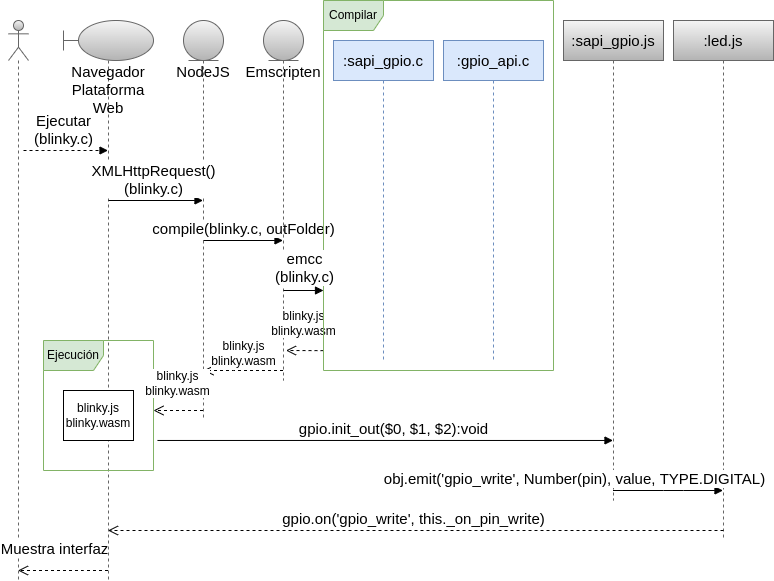
\includegraphics[scale=.49]{./Figures/DiagramaSecuencia.png}
	\caption{Interacción del usuario con las dependencias del emulador.}
	\label{fig:DiagramaSecuencia}
\end{figure}

Además, la capa \textit{JavaScript HAL}, que interactúa con el código \textit{JavaScript} resultante de la compilación de la \textit{Biblioteca C} y \textit{C HAL}, se encarga de notificar los eventos ocurridos en esas capas para el programa de usuario \texttt{blinky}. Mediante la función \texttt{write}, se realiza la activación del evento que escribe en la GPIO, Como resultado, emitirá el evento con el nombre \texttt{gpio\_write}, pasando como argumentos el número de pin, el valor digital y el tipo de pin declarado.


La figura \ref{fig:GPIOEventEmitter} muestra el diagrama en bloques del evento con el nombre \newline \texttt{gpio\_write}.

\begin{figure}[ht]
	\centering
	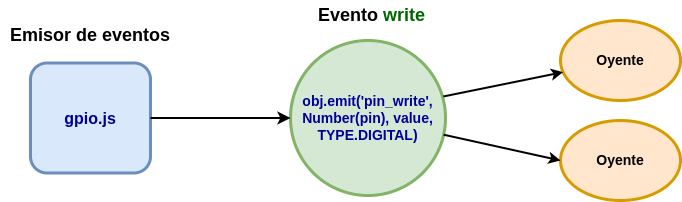
\includegraphics[scale=.40]{./Figures/GPIOEventEmitter.png}
	\caption{Activación de evento con el nombre \texttt{gpio\_write}.}
	\label{fig:GPIOEventEmitter}
\end{figure}



En ese sentido, en la capa \textit{JavaScript UI}  cuando se emite el evento con el nombre \texttt{gpio\_write}, cualquier oyente que esté suscrito a ese evento podrá escucharlo y realizar las acciones correspondientes para la funcionalidad que se requiere. En este caso, la acción solicitada es encender el LED.

La figura \ref{fig:ListeningGPIOEventEmitter} muestra el diagrama en bloques del oyente subscrito al evento \texttt{gpio\_write}.


\begin{figure}[ht]
	\centering
	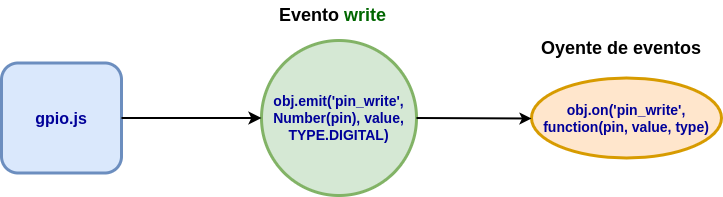
\includegraphics[scale=.40]{./Figures/ListeningGPIOEventEmitter.png}
	\caption{GPIO oyente del evento con el nombre \texttt{gpio\_write}.}
	\label{fig:ListeningGPIOEventEmitter}
\end{figure}

Entonces, en la plataforma web se muestrarán los cambios de \texttt{gpio\_write} en la placa virtual. 

En la figura \ref{fig:AplicacionUsuarioLeds} se presenta para una función de la GPIO, la interacción entre todas las capas de programación.


\begin{figure}[ht]
	\centering
	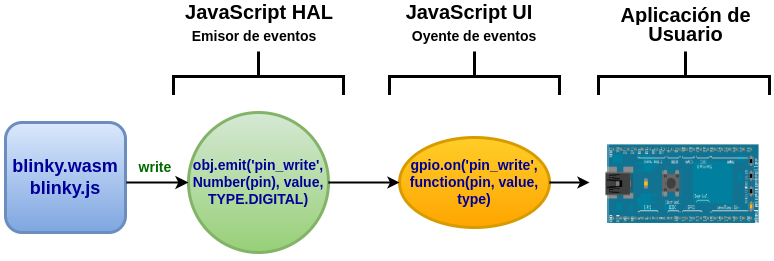
\includegraphics[scale=.36]{./Figures/AplicacionUsuarioLeds.png}
	\caption{Interacción entre todas las capas de programación.}
	\label{fig:AplicacionUsuarioLeds}
\end{figure}


\section{Despliegue}


Para hacer público el emulador de la plataforma en un servidor web, se realizó el proceso de despliegue en el servidor de \textit{DigitalOcean} mediante los siguientes pasos:


\begin{itemize}
	\item Crear una cuenta: implicó registrar una cuenta en la plataforma. Después de iniciar sesión, se creo un \textit{droplet}, que es un servidor virtual. Luego, se instaló el sistema operativo \textit{Ubuntu}, y se configuró la región geográfica donde se ubicaría el servidor y la cantidad de RAM.
	
	\item Acceso al servidor: después que el \textit{droplet} fue creado, se pudo  obtener la dirección IP pública y la clave \textit{SSH} para acceder al servidor.
	
	\item Configuración: implicó instalar las herramientas, como \textit{Mbed CLI} y \textit{Emscripten}, y también, los servicios necesarios, como los entornos de ejecución de \textit{Node.js} y \textit{Python}. Además, se realizó las configuraciones de las reglas de \textit{firewall}.

	\item Copiar la plataforma web al servidor: se utilizó \textit{GitHub}  para clonar el repositorio en el servidor. El código del presente trabajo, se encuentra en el repositorio de GitHub \citep{repositorioEmulador}.
	
	\item Iniciar el emulador web: se utilizó la herramienta \textit{TMUX} para mantener la sesión y la ventana de la terminal donde se ejecuta la aplicación de forma persistente, incluso cuando se cierra la conexión  \textit{SSH}. El presente trabajo, se encuentra actualmente ejecutandose en 
\url{http://134.209.168.175:7900}.
\end{itemize}






% Chapter Template

\chapter{Ensayos y resultados} % Main chapter title

\label{Chapter4} % Change X to a consecutive number; for referencing this chapter elsewhere, use \ref{ChapterX}

En este capítulo se presentan las pruebas realizadas para comprobar el funcionamiento de la plataforma de emulación y las diferencias que presenta con respecto a la placa real. Además, se describen las diferentes herramientas que se utilizaron.
%----------------------------------------------------------------------------------------
%	SECTION 1
%----------------------------------------------------------------------------------------

\section{Banco de pruebas}

Para verificar el funcionamiento de la plataforma de emulación se emplearon diversos recursos de software y hardware, que permitió una evaluación completa del funcionamiento de la plataforma de emulación, garantizando su confiabilidad y funcionalidad. 

El proceso de verificación incluyó también pruebas comparativas entre la plataforma de emulación y la placa física, donde se ejecutaron casos de prueba idénticos en ambos entornos. Esto permitió identificar y analizar las diferencias entre el comportamiento real y la del emulador web, además, proporcionó información valiosa para mejorar la precisión y fiabilidad de la plataforma web de emulación.



En la tabla \ref{tab:RecursosHardware} se presentan los recursos de hardware empleados en el banco de pruebas.

\begin{table}[h]
	\centering
	\caption[Recursos de hardware utilizados]{Recursos de hardware utilizados.}
	\begin{tabular}{l c}    
		\toprule
		\textbf{Herramienta} & \textbf{Propósito}\\
		\midrule
		Computadora & Acceso a la plataforma de emulación.\\		
		Placa EDU-CIAA-NXP &  Implementación de los ejemplos de la sAPI.\\
		Dht11 temperature \& humidity  &  Pruebas de ejemplo.\\
		\bottomrule
		\hline
	\end{tabular}
	\label{tab:RecursosHardware}
\end{table}


Asimismo, se utilizaron herramientas de software para realizar las pruebas
en todos los módulos que componen el sistema. En la tabla \ref{tab:RecursosSoftware} se describe el propósito de estas herramientas.

\hfill \break
\hfill \break
\hfill \break
\hfill \break

\begin{table}[h]
	\centering
	\caption[Recursos de software utilizados]{Recursos de software utilizados.}
	\begin{tabular}{l c}    
		\toprule
		\textbf{Herramienta} & \textbf{Propósito}\\
		\midrule
		Mocha &  Pruebas automatizadas para el frontend.\\		
		Chai &   Pruebas automatizadas para el frontend.\\
		Chrome & Pruebas de la plataforma web.\\
		Firefox & Pruebas de la plataforma web.\\
		Explorer &  Pruebas de la plataforma web. \\
		PostMan \citep{Postman} &  Pruebas de \textit{request} de la plataforma y APIs. \\
		CMocka &  Pruebas automatizadas para el backend. \\
		GCC  & Para la compilación de las pruebas de backend. \\
		Check  & Para la ejecución de las pruebas de backend. \\
		Mocha  &  Pruebas automatizadas para el frontend. \\
		Chai  &  Pruebas automatizadas para el frontend. \\
        Tera Term \citep{TeraTerm} &  Emulador de la terminal serial. \\
		\bottomrule
		\hline
	\end{tabular}
	\label{tab:RecursosSoftware}
\end{table}

\section{Pruebas de Unidad} 
\label{subsec:Pruebas de Unidad}  

Las pruebas de unidad se centraron en evaluar de manera aislada cada método de los archivos de código fuente de la biblioteca C, con el objetivo de que cada unidad de código funcione correctamente y produzca los resultados esperados. 

Asimismo, para el desarrollo de las pruebas unitarias, se utilizaron \textit{Check} y \textit{CMocka}, que son bibliotecas de pruebas unitarias escritas en lenguaje \textit{C}. \textit{CMocka} proporcionó funcionalidades para simular o mockear las funciones y dependencias externas de \textit{emscripten}, lo que posibilitó enfocarse en probar exclusivamente los módulos de la biblioteca C.

Además, para compilar las pruebas unitarias con \textit{CMocka} o \textit{Check}, se utilizó el compilador \textit{GCC (GNU Compiler Collection)}. El proceso consiste en compilar los archivos fuente de las pruebas y generar un archivo ejecutable que contiene el resultado del proceso de compilación y enlazado. Los resultados de las pruebas unitarias se mostrarán en la consola al ejecutar el archivo ejecutable generado.

Por ejemplo, la consola indicará lo siguiente:

\begin{itemize}
	\item El porcentaje de pruebas probadas.
	\item La cantidad de pruebas que aprobaron.
	\item La cantidad de pruebas que fallaron.
	\item Si alguna prueba falla, entonces, indicara el error específico.
	\item Si alguna prueba falla, proporcionará detalles adicionales para identificar el problema.
\end{itemize}

Se desarrollaron estas pruebas y se registraron los resultados en la consola. La figura \ref{fig:PruebasUnidad1} muestra la primera parte de la salida por consola durante la depuración de las pruebas unitarias y la figura \ref{fig:PruebasUnidad2} muestra la segunda parte.

\begin{figure}[ht]
	\centering
	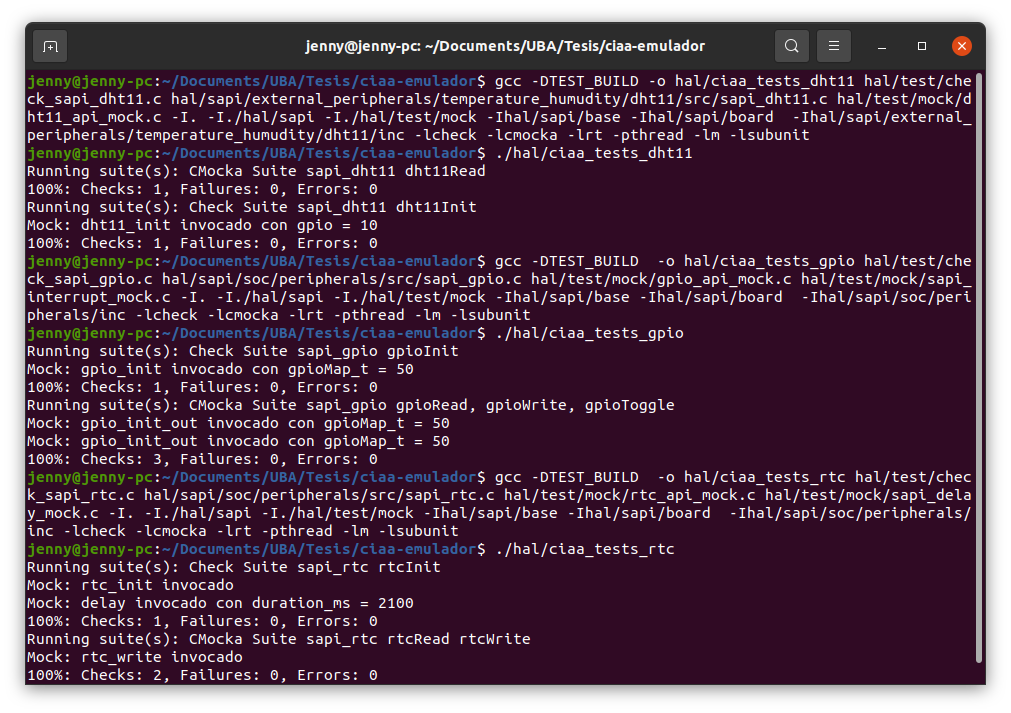
\includegraphics[scale=.27]{./Figures/PruebasUnidad1.png}
	\caption{Primera parte de la salida por consola de las pruebas unitarias con \textit{CMocka} o \textit{Check}.}
	\label{fig:PruebasUnidad1}
\end{figure}


\begin{figure}[ht]
	\centering
	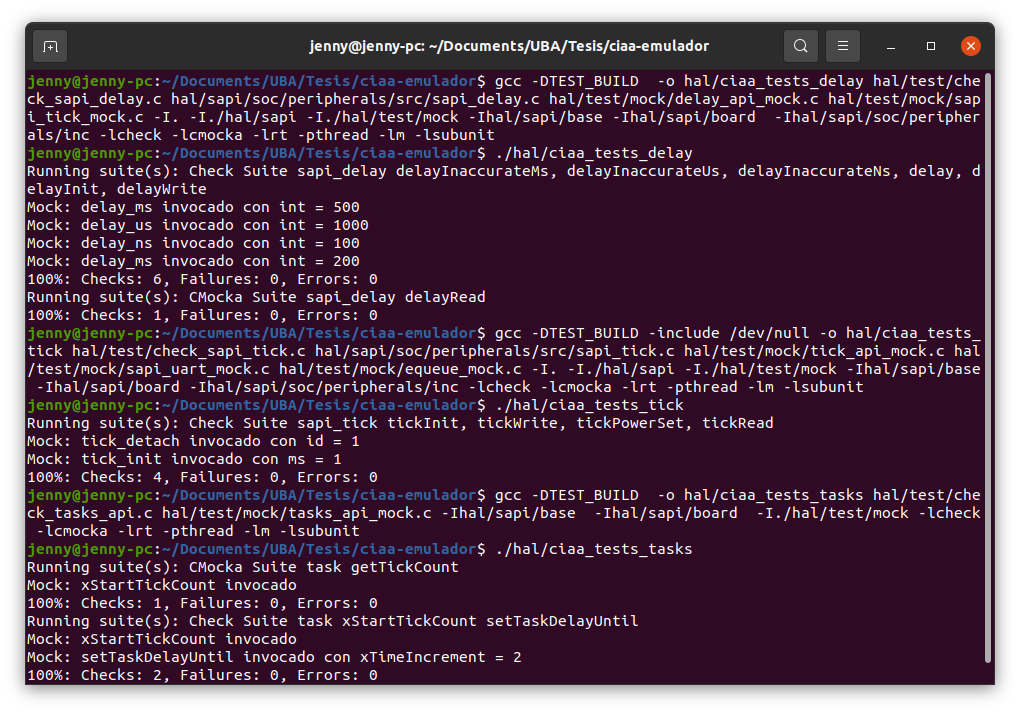
\includegraphics[scale=.27]{./Figures/PruebasUnidad2.png}
	\caption{Segunda parte de la salida por consola de las pruebas unitarias con \textit{CMocka} o \textit{Check}.}
	\label{fig:PruebasUnidad2}
\end{figure}
 

\section{Pruebas de Integración} 
\label{subsec:Pruebas de Integración}

Las pruebas de integración se centran en evaluar la interacción y comunicación entre diferentes componentes. Además, asegura que trabajen en conjunto sin problemas.

A medida que se fueron desarrollando diferentes módulos y funcionalidades del emulador, las pruebas de integración fueron necesarias para identificar posibles conflictos o incompatibilidades entre los distintos componentes de código del emulador web.

Se fueron identificando las interacciones entre componentes que fueron relevantes a partir de las pruebas de unidad existentes, como \texttt{sapi\_delay} y \texttt{sapi\_tick}. Luego, se identificaron las dependencias de \textit{Emscripten} y las funciones que se invocan entre las diferentes pruebas de unidad.

Luego, se crearon archivos de prueba de integración con escenarios especificos que combinen las interacciones entre los componentes y se utilizaron \textit{mocks} para simular comportamientos de funciones de \textit{Emscripten}.

Al igual que en las pruebas de unidad se utilizo el compilador GCC para compilar. A continuacion la figura \ref{fig:PruebasIntegracion} muestra los resultados por consola de las pruebas de integracion.

\begin{figure}[ht]
	\centering
	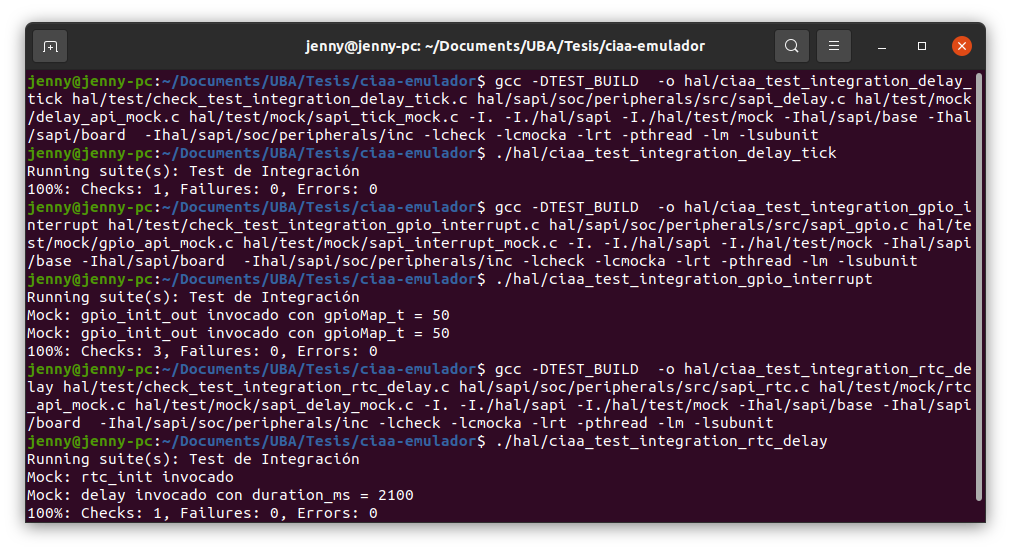
\includegraphics[scale=.35]{./Figures/PruebasIntegracion.png}
	\caption{Depuración de las pruebas de integracion.}
	\label{fig:PruebasIntegracion}
\end{figure}

\section{Pruebas de Interfaz}
\label{sec:Pruebas de Interfaz}

Para lograr que la interfaz de la plataforma de emulación cumpla con los requisitos funcionales y logre que los usuarios lo adopten con éxito fue necesario implementar las pruebas de la interfaz de usuario.

Por tanto, se implementaron pruebas automatizadas que verifiquen que el funcionamiento sea el correcto, tanto desde la interacción con el usuario así como también con las peticiones hacia el backend.

La implementación de estas pruebas automatizadas permitió que se  ejecuten de forma rápida y confiable de manera recurrente. 

Para automatizar las pruebas de la interfaz de usuario con \textit{\textbf{NodeJS}}, se utilizó en el desarrollo las bibliotecas \textit{\textbf{Mocha}} y \textit{\textbf{Chai}}, que permitieron crear pruebas de interfaz muy completas para el desarrollo en \textit{JavaScript}.

Además, permitió asegurar que cada componente de la interfaz funcione correctamente por separado. Incluso, verificó si el código en el navegador web devolvió los nombres de los módulos correctos, los tipos de parámetros previstos y el tipo de retorno esperado.

La figura \ref{fig:TestVS1} muestra la salida por consola durante la depuración de las pruebas de interfaz con \textit{\textbf{Mocha}}.


\begin{figure}[ht]
	\centering
	\includegraphics[scale=.29]{./Figures/TestInterfaz.png}
	\caption{Salida por consola durante la depuración de las pruebas de interfaz con \textit{\textbf{Mocha}}.}
	\label{fig:TestVS1}
\end{figure}

\section{Integracion Continua}
\label{sec:Integracion Continua}

Para implementar la integración continua del código se evaluaron dos plataformas: GitLab CI y Travis CI. Ambas herramientas, proporcionaron excelentes resultados y demostraron ser igualmente eficaces. Sin embargo, se encontraron algunas diferencias importantes en su configuración y en cómo se presentan las pruebas en cada plataforma.

En el caso de GitLab CI, toda la configuración se realizó directamente en la plataforma de GitLab, lo que facilitó la integración con el repositorio de la plataforma web y permitió una gestión más centralizada del proceso de CI/CD.

Por otro lado, con Travis CI, se realizaron configuraciones separadas de GitHub. Esto implicó un enfoque más descentralizado, lo que puede ser útil si se trabaja en varios proyectos alojados en diferentes repositorios.

Después de evaluar ambas opciones, se decidió utilizar ambas tecnologías, dado que son gratuitas para código abierto. Además, esta elección brindó mayor flexibilidad y resguardo en caso de problemas con alguna de estas herramientas.

En general, la experiencia con ambas herramientas fue positiva y permite mejorar la calidad y eficiencia del proceso de desarrollo mediante la automatización de las pruebas unitarias y de integracion, Además de los despliegues continuos.

En ambas plataformas, la información que se muestra en la consola proporciona la siguiente información útil:

\begin{itemize}
	\item Resultado de las pruebas: la consola muestra si las pruebas se ejecutaron con éxito o si hubo fallas en alguna de ellas. 
	
	\item Detalle de los fallos: en el caso de que alguna prueba falle, la consola proporcionará información detallada, como el nombre de la prueba, el nombre del archivo y la línea de código donde ocurrió el error.
	
	\item Información sobre el entorno de prueba: la consola muestra detalles sobre el entorno de prueba utilizado tanto en Travis CI  como en GitLab CI, que incluye la versión del lenguaje de programación, la secuencia de dependencias instaladas y otros detalles de las pruebas.
	
	\item Duración de las pruebas: la consola muestra el tiempo que tardaron todas las pruebas en ejecutarse,  de manera que, permite identificar las pruebas que deben ser modificadas para optimizar su rendimiento.
	
	\item Logs de ejecución: la consola mostrará registros detallados de la ejecución de las pruebas, que incluyen mensajes del progreso de las pruebas, información de depuración y los resultados de las pruebas.
	
\end{itemize}

La siguiente figura \ref{fig:travis} presenta la consola de Travis CI.  

\begin{figure}[ht]
	\centering
	\includegraphics[scale=.35]{./Figures/travis.png}
	\caption{Información de las pruebas que se ejecutaron en Travis CI.}
	\label{fig:travis}
\end{figure}


La figura \ref{fig:gitLab} presenta la consola de GitLab CI.  

\begin{figure}[ht]
	\centering
	\includegraphics[scale=.40]{./Figures/gitLab.png}
	\caption{Información de las pruebas que se ejecutaron en GitLab CI.}
	\label{fig:gitLab}
\end{figure}

\hfill \break
\hfill \break
\hfill \break
\hfill \break
\hfill \break



\subsection{Prueba de acceso}    

Para verificar y validar el acceso mediante solicitudes HTTP al servidor donde se encuentra publicado el emulador de la plataforma web, se utilizó la herramienta Postman.

Antes de comenzar con el ensayo, se creó un caso de prueba con el propósito de ser una guía estructurada y documentada para verificar si el acceso al servidor funciona como se espera.


\textit{\textbf{ID Caso de prueba: CP01}}

Descripción: la primera vez que el usuario ingresa a la plataforma de emulación se muestra en ejecución el ejemplo predeterminado \textit{Blinky}.

Pre-condición: 
\begin{itemize}
	\item La computadora del usuario tiene conexión a internet y un navegador web instalado.
\end{itemize}

Flujo principal:
\begin{itemize}
	\item El usuario ingresa al entorno web de la plataforma de emulación para la placa EDU-CIAA-NXP.
\end{itemize}
Post condiciones:
\begin{itemize}
	\item ÉXITO: la plataforma muestra el ejemplo \textit{\textbf{Blinky}} en ejecución al encender y apagar el LEDB.
	\item FALLA: La plataforma no muestra ningún ejemplo predeterminado en ejecución.
\end{itemize}

Resumen del Test:
\begin{itemize}
	\item Después de acceder a la plataforma mediante los navegadores web Chrome, Firefox y Explorer se comprobó que se muestra en ejecución el ejemplo \textit{\textbf{Blinky}}.
	\item Se realizó la prueba de HTTP \textit{requests} por medio de la utilización de la herramienta \textit{\textbf{Postman}} que luego de acceder a la dirección del servidor donde se encuentra la plataforma, devolvió en formato \textit{\textbf{JSON}} la respuesta del servidor.
\end{itemize}


La figura \ref{fig:PlataformaEmuladorBlinky} muestra la plataforma de emulación ejecutando el ejemplo predeterminado \textit{\textbf{Blinky}}.

\begin{figure}[ht]
	\centering
	\includegraphics[scale=.21]{./Figures/PlataformaEmuladorBlinky.png}
	\caption{Prueba plataforma emulador ejecutando el ejemplo \textit{\textbf{Blinky}}.}
	\label{fig:PlataformaEmuladorBlinky}
\end{figure}

\textit{\textbf{Postman}} es una aplicación que permite realizar pruebas API. La herramienta permitió realizar pruebas \textit{\textbf{HTTP requests}} y acceder al servidor de la plataforma de emulación. Se obtuvo la respuesta en diferentes formatos como  \textit{\textbf{JSON}}, \textit{\textbf{XML}}, \textit{\textbf{HTML}} y \textit{\textbf{Text}}.


En la figura \ref{fig:PostmanBlinky2} se muestra la petición y respuesta de acceso a la plataforma por medio de la herramienta \textit{\textbf{Postman}}.

\hfill \break
\hfill \break
\hfill \break
\hfill \break
\hfill \break
\hfill \break
\hfill \break
\hfill \break
\hfill \break
\hfill \break

\begin{figure}[ht]
	\centering
	\includegraphics[scale=.40]{./Figures/PostmanBlinky2.png}
	\caption{Respuesta del servidor.}
	\label{fig:PostmanBlinky2}
\end{figure}


\section{Pruebas de funcionamiento}  
\label{sec:Pruebas de funcionamiento}

Para evaluar, verificar el comportamiento y desempeño del microcontrolador en el entorno web, se realizan a continuación pruebas funcionales con uno de los periféricos internos seleccionados, que es el RTC. Además, se elige para la prueba un periférico externo, el DHT11.

También, se realiza una prueba de un nuevo proyecto \textquotedbl tick hook\textquotedbl, que muestra las diferencias en el funcionamiento y los resultados obtenidos entre la plataforma web y la placa física EDU-CIAA-NXP.

\subsection{ Prueba del ejemplo \textit{\textbf{rtc printf}}}

Para el ensayo en la plataforma de emulación web se siguió con los pasos del siguiente caso de uso:

\textit{\textbf{ID Caso de prueba: CP02}}

Descripción: la plataforma de emulación permite al usuario ejecutar el ejemplo \textit{\textbf{rtc printf}}.

Pre-condición: 
\begin{itemize}
	\item La computadora del usuario tiene conexión a internet y un navegador web instalado.
\end{itemize}

Flujo principal:
\begin{enumerate}
	\item El usuario ingresa al entorno web de la plataforma de emulación para la placa EDU-CIAA-NXP.
	\item El usuario selecciona desde la lista desplegable el ejemplo \textit{\textbf{rtc printf}}.
	\item La plataforma muestra en pantalla al usuario el código que corresponde al ejemplo \textit{\textbf{rtc printf}}.
	\item El usuario hace click en el botón \textquotedbl Ejecutar\textquotedbl.
	\item La plataforma muestra en la consola integrada la salida del rtc.
	\item El usuario realiza la descarga del ejemplo \textit{\textbf{rtc printf}} al hacer click en el botón de descarga, ubicado en el área de codificación.

\end{enumerate}


Post condiciones:
\begin{itemize}
	\item ÉXITO: la plataforma muestra en ejecución el ejemplo \textit{\textbf{rtc printf}} al actualizar la salida por consola del envío por UART.
	\item FALLA: La plataforma no muestra al usuario ningún cambio en la consola.
\end{itemize}


Luego de completar el caso de uso CP02, se obtuvo el siguiente resultado: 

\begin{itemize}
	\item ÉXITO: la plataforma muestra en ejecución el ejemplo \textit{\textbf{rtc printf}}.
\end{itemize}


La figura \ref{fig:rtcprintf} muestra en la consola integrada la salida del ensayo. 

\begin{figure}[ht]
	\centering
	\includegraphics[scale=.21]{./Figures/rtcprintf.png}
	\caption{Salida por consola del ensayo \textit{\textbf{rtc printf}}.}
	\label{fig:rtcprintf}
\end{figure}

\subsubsection{Ensayo en la placa EDU-CIAA-NXP} 

Primeramente, dentro de la herramienta de desarrollo \textit{eclipse} se importa el archivo \textquotedbl rtc\_printf.c\textquotedbl{} generado por la plataforma web, luego, se realiza las configuraciones necesarias para compilar el proyecto. 

La figura \ref{fig:rtcprintfEclipse} expone el ejemplo \textit{\textbf{rtc printf}} importado en \textit{eclipse}: 

\begin{figure}[ht]
	\centering
	\includegraphics[scale=.20]{./Figures/rtcprintfEclipse.png}
	\caption{Ejemplo \textit{\textbf{rtc printf}} importado en \textit{eclipse}.}
	\label{fig:rtcprintfEclipse}
\end{figure}

\hfill \break
\hfill \break
\hfill \break
\hfill \break
\hfill \break
\hfill \break
\hfill \break
\hfill \break


Finalmente, se ejecuta el mismo ejemplo en la placa física EDU-CIAA-NXP y se obtiene por consola la siguiente salida que se muestra en la figura \ref{fig:rtcprintfPlaca}:

\begin{figure}[ht]
	\centering
	\includegraphics[scale=.90]{./Figures/rtcprintfPlaca.png}
	\caption{Salida de la terminal COM7 -Tera Term VT.}
	\label{fig:rtcprintfPlaca}
\end{figure}



Resumen de la prueba Exitosa:
\begin{itemize}
	\item Después de seguir los pasos del flujo principal del caso de prueba, se comprobó que se muestra en ejecución el ejemplo \textit{\textbf{rtc printf}}.
	\item El ensayo en la placa física EDU-CIAA-NXP  con el mismo ejemplo \textit{\textbf{rtc printf}} obtuvo la misma salida por consola de la plataforma web.

\end{itemize}


\subsection{Prueba del ejemplo \textit{\textbf{dht11}} }

\subsubsection{Ensayo en la plataforma de emulación web} 
Para el ensayo en la plataforma de emulación web se siguió con los pasos del siguiente caso de uso:

\textit{\textbf{ID Caso de prueba: CP03}}

Descripción: la plataforma de emulación permite al usuario ejecutar el ejemplo \textit{\textbf{dht11}}.

Pre-condición: 
\begin{itemize}
	\item La computadora del usuario tiene conexión a internet y un navegador web instalado.
\end{itemize}

Flujo principal:
\begin{enumerate}
	\item El usuario ingresa al entorno web de la plataforma de emulación para la placa EDU-CIAA-NXP.
	\item El usuario selecciona desde la lista desplegable jerárquica el ejemplo \textit{\textbf{dht11}}.
	\item La plataforma web realiza las siguientes acciones:
	 
	\begin{itemize}
	    \item muestra al usuario el código  del ejemplo \textit{\textbf{dht11}} dentro del área de codificación.
	    \item carga el periférico virtual de manera automática dentro del área de ensamblado y muestra las conexiones a los pines configurados por defecto, los cuales son: \textquotedbl SIGNAL=GPIO1\textquotedbl, \textquotedbl SDA/SDI=GND\textquotedbl{} y \textquotedbl VCC=3V3\textquotedbl.
	    \item muestra seleccionado la opción por defecto \textquotedbl Obtener datos de servidor climático local.\textquotedbl
	    \item actualiza los termómetros gráficos que corresponden a la temperatura y a la humedad con los datos obtenidos del servidor climático.
	\end{itemize}

	\item El usuario hace click en el botón \textquotedbl Ejecutar\textquotedbl.
	\item La plataforma muestra en la consola integrada la salida de la temperatura y humedad con los valores enviados desde la central meteorológica en línea.
	\item El usuario realiza la descarga del ejemplo \textit{\textbf{dht11}} al hacer click en el botón de descarga, ubicado en el área de codificación.
\end{enumerate}

Flujo alternativo:
\begin{enumerate}
    \setcounter{enumi}{3}
	\item El usuario hace clic en la opción \textquotedbl Establecer Temperatura y Humedad manualmente(haga click y arrastre sobre
los indicadores).\textquotedbl
	\item La plataforma deselecciona la opción \textquotedbl Obtener datos de servidor climático local.\textquotedbl
    \item El usuario comienza a manipular los termómetros gráficos haciendo clic sobre los que corresponden a la temperatura y a la humedad.
    \item La plataforma actualiza los termómetros gráficos que corresponden a la temperatura y a la humedad con los datos generados por el usuario.

	\item El usuario hace click en el botón \textquotedbl Ejecutar\textquotedbl.
	
	\item La plataforma muestra en la consola integrada la salida de la temperatura y humedad según la selección de obtención de datos.
	
	\item El usuario realiza la descarga del ejemplo \textit{\textbf{dht11}} al hacer click en el botón de descarga, ubicado en el área de codificación.
\end{enumerate}



Post condiciones:
\begin{itemize}
	\item ÉXITO: la plataforma debe cumplir con todas las siguientes condiciones de éxito:
	
		\begin{itemize}
	    \item  carga automáticamente el periférico virtual dentro del área de ensamblado y las conexiones configuradas por defecto.
	    
	    \item actualiza los termómetros gráficos de  temperatura y  humedad, que  corresponden a la elección de obtención de datos.

	    \item muestra en ejecución el ejemplo \textit{\textbf{dht11}} y según la elección de obtención de datos, actualiza la salida de temperatura y humedad en la consola integrada.
	    \end{itemize}
	
	\item FALLA: la plataforma no cumple con todas las condiciones de éxito descritas.
\end{itemize}

Luego de completar el caso de uso CP02 con: flujo principal y flujo alternativo, se obtuvo el siguiente resultado: 

\begin{itemize}
	\item ÉXITO: la plataforma cumple con todas las condiciones de éxito para el ejemplo \textit{\textbf{dht11}}.
\end{itemize}

La figura \ref{fig:RespuestaEmulador} muestra la consola con los datos de temperatura y humedad del ejemplo \textit{\textbf{dht11}} con la opción \textquotedbl  Establecer Temperatura y Humedad manualmente(haga click y arrastre sobre
los indicadores).\textquotedbl


\begin{figure}[ht]
	\centering
	\includegraphics[scale=.20]{./Figures/dht11Opcion2.png}
	\caption{Resultado del CP02 con la opción \textquotedbl Establecer Temperatura y Humedad manualmente(haga click y arrastre sobre
los indicadores).\textquotedbl}
	\label{fig:RespuestaEmulador}
\end{figure}


La figura \ref{fig:RespuestaEmulador} muestra la consola con los datos de temperatura y humedad del ejemplo \textit{\textbf{dht11}} con la opción \textquotedbl Obtener datos de servidor climático local.\textquotedbl


\begin{figure}[ht]
	\centering
	\includegraphics[scale=.20]{./Figures/dht11Opcion1.png}
	\caption{Resultado del  CP02 con la opción \textquotedbl Obtener datos de servidor climático local.\textquotedbl}
	\label{fig:RespuestaEmulador}
\end{figure}




Para verificar que la plataforma obtuvo los datos de temperatura/humedad de la API de meteorología  \textit{\textbf{openweathermap}} se hicieron pruebas de \textit{request} con la herramienta \textit{Postman}.

En la figura \ref{fig:RespuestaPostMan1} se observa que la petición de datos de temperatura/humedad recibe como parámetro la ciudad que se quiere consultar.



\begin{figure}[ht]
	\centering
	\includegraphics[scale=.30]{./Figures/RespuestaPostMan1.png}
	\caption{Petición de datos de temperatura/humedad.}
	\label{fig:RespuestaPostMan1}
\end{figure}

En este paso se verifica que la respuesta de la petición de datos de temperatura/humedad al API \textit{\textbf{openweathermap}} coincide con lo que se observó en la terminal de la plataforma de emulación.


\subsubsection{Ensayo en la placa EDU-CIAA-NXP} 

Este ensayo tuvo como objetivo identificar
las diferencias entre los resultados reales producidos por la placa física EDU-CIAA-NXP y los resultados esperados en la plataforma de emulación.

El primer paso fue conectar el componente dht11 a la placa EDU-CIAA-NXP. En consecuencia, se procedió a importar el archivo generado por la plataforma web  \textquotedbl dht11\_temp\_humidity.c\textquotedbl{} y compilarlo                     dentro de la herramienta 
\textit{eclipse}. Luego, se grabó en la placa física EDU-CIAA-NXP.

A continuación se muestra en la figura \ref{fig:TestHardware} la ejecución del ensayo en la plataforma EDU-CIAA-NXP.

\begin{figure}[ht]
	\centering
	\includegraphics[scale=.45]{./Figures/TestHardware.jpeg}
	\caption{Ensayo en la plataforma EDU-CIAA-NXP del ejemplo \textit{\textbf{dht11}}.}
	\label{fig:TestHardware}
\end{figure}



La figura \ref{fig:TestEclipse} muestra el código del ejemplo \textit{\textbf{dht11}} en la herramienta \textit{eclipse} de la PC de prueba.

\begin{figure}[ht]
	\centering
	\includegraphics[scale=.20]{./Figures/TestEclipse.png}
	\caption{Código del ejemplo en eclipse.}
	\label{fig:TestEclipse}
\end{figure}


El programa \textit{\textbf{dht11}} de la plataforma de emulación es un ejemplo simple que solo enciende el LEDG en la placa y además, lee los datos generados del sensor Dht11 que consisten en temperatura/humedad. Luego, los datos leídos se imprimen por pantalla. 

En este ensayo manual se registraron los cambios en la placa EDU-CIAA-NXP y también, los mensajes de la terminal serie. De modo que, posteriormente, permitió compararlos con la plataforma de emulación.

En la figura \ref{fig:TestPlaca} se observan los cambios en la placa EDU-CIAA-NXP que fueron registrados durante las pruebas.


\begin{figure}[ht]
	\centering
	\includegraphics[scale=.50]{./Figures/TestPlaca.jpeg}
	\caption{Cambios en la placa EDU-CIAA-NXP durante el ensayo.}
	\label{fig:TestPlaca}
\end{figure}


Ahora bien, para leer los datos por pantalla se utilizó la herramienta \textit{Tera Term VT} que permitió levantar los datos de temperatura/humedad.

En la figura \ref{fig:TestTerminal} se muestra los datos de temperatura/humedad usando \textit{Tera Term VT}. 


\begin{figure}[ht]
	\centering
	\includegraphics[scale=.90]{./Figures/TestTerminal.png}
	\caption{Salida de la terminal COM7 -Tera Term VT.}
	\label{fig:TestTerminal}
\end{figure}



Resumen de la prueba Exitosa:
\begin{itemize}
	\item Después de acceder a la plataforma mediante el navegador y siguiendo los pasos del flujo principal y el flujo alternativo de la prueba, se comprobó que se muestra en ejecución el ejemplo \textit{\textbf{Dht11 temperature/humidity}}.
	\item Se realizó la prueba de HTTP \textit{requests} usando la herramienta \textit{\textbf{Postman}} para comprobar la respuesta del \textit{\textbf{API openweathermap}} que consume la plataforma de emulación de manera que, los datos de temperatura y humedad sean los mismos.
	\item Se ensayo en la placa física EDU-CIAA-NXP  el mismo ejemplo \textit{\textbf{Dht11 temperature/humidity}} y se registraron los resultados de la terminal serial.

\end{itemize}


\subsection{ Prueba de un nuevo proyecto \textit{\textbf{tick hook}}}
El objetivo de este ensayo es exponer las diferencias en los resultados encontrados entre el emulador web y la placa física EDU-CIAA-NXP.

\subsubsection{Ensayo en la plataforma de emulación web} 
Para ensayar la plataforma web, se ejecuto el siguiente caso de prueba:

\textit{\textbf{ID Caso de prueba: CP04}}

Descripción: la plataforma de emulación permite al usuario ejecutar un nuevo ejemplo de \textit{\textbf{tick hook}}.

Pre-condición: 
\begin{itemize}
	\item La computadora del usuario tiene conexión a internet y un navegador web instalado.
\end{itemize}

Flujo principal:
\begin{enumerate}
	\item El usuario ingresa al entorno web de la plataforma de emulación para la placa EDU-CIAA-NXP.
	\item El usuario hace click en el botón \textquotedbl Nuevo Proyecto\textquotedbl.
	\item La plataforma muestra al usuario en el área de codificacion, la pantalla para que pueda ingresar su propio codigo.
	\item El usuario ingresa el siguiente código de prueba:
	
\begin{lstlisting}[caption={nuevo proyecto}]
#include "sapi.h"

void myTickHook( void *ptr )
{
   gpioWrite( LED3, ON );
   printf( "Blinky LED3.\r\n" );
   while(TRUE) {
      printf( " while(TRUE)  Blinky LED1.\r\n" );
      gpioToggle( LED1 );
      delay(1);
   }
}

int main()
{
    boardConfig();
    tickInit(50);
    while ( TRUE )
    {
		tickCallbackSet( myTickHook, NULL );
		delay(5000);
    }
    return 0;
}
\end{lstlisting}

	\item El usuario hace click en el botón \textquotedbl Ejecutar\textquotedbl.
	\item La plataforma muestra en la consola integrada la salida del programa en ejecución.
	
\end{enumerate}
	

La figura \ref{fig:Testtickhook} muestra en la consola integrada la salida de \textquotedbl Blinky LED3\textquotedbl muchas veces. 


\begin{figure}[ht]
	\centering
	\includegraphics[scale=.20]{./Figures/Testtickhook.png}
	\caption{Salida por consola del ensayo tick hook.}
	\label{fig:Testtickhook}
\end{figure}

\subsubsection{Ensayo en la placa EDU-CIAA-NXP} 

Se ejecuta el mismo ejemplo en la placa física EDU-CIAA-NXP y se obtiene por consola la siguiente salida que se muestra en la siguiente figura \ref{fig:TesttickhookPlaca}:


\begin{figure}[ht]
	\centering
	\includegraphics[scale=.80]{./Figures/TesttickhookPlaca.png}
	\caption{Salida de la terminal COM7 -Tera Term VT.}
	\label{fig:TesttickhookPlaca}
\end{figure}

\hfill \break
\hfill \break
\hfill \break
\hfill \break
\hfill \break
\hfill \break
\hfill \break
\hfill \break
\hfill \break
\hfill \break
\hfill \break
\hfill \break
\hfill \break
Se observa que la salida por consola de \textquotedbl Blinky LED3\textquotedbl se muestra solo una vez, lo cual difiere de la salida por consola de la plataforma web que muestra \textquotedbl Blinky LED3\textquotedbl{} muchas veces.

La diferencia de este comportamiento en el emulador web esta relacionada con la forma en cómo JavaScript reanuda la ejecución después de que ocurre un tick. Por lo tanto, la forma en que se gestionan los estados en la ejecución de funciones puede diferir del comportamiento en la placa EDU-CIAA-NXP.

En un entorno físico, el sistema operativo o el microcontrolador pueden mantener un seguimiento del estado de la ejecución y reanudarla adecuadamente después de una interrupción o tick del sistema. Sin embargo, para esta prueba en particular, dentro de la plataforma de emulación web, no se mantiene este estado de ejecución, lo que resulto la repetición de ciertas porciones de código, como se probó anteriormente.

Para solucionar esta diferencia en el entorno del emulador web, se podría explorar algunas opciones para mantener un seguimiento adecuado del estado de ejecución después de que ocurra un tick del sistema.

\subsection{Periféricos implementados en \textit{Mbed Simulator} y en el Emulador EDU-CIAA-NXP}

La siguiente tabla \ref{tab:perifericosInternosMBED} expone los  periféricos internos implementados actualmente en \textit{Mbed Simulator}.

\begin{table}[h]
\centering
\caption[Comparación de características de periféricos internos implementados en \textit{Mbed Simulator}]{Comparación de características de Periféricos internos implementados en \textit{Mbed Simulator}}
\begin{tabular}{p{0.24\linewidth} p{0.14\linewidth}  p{0.14\linewidth}  p{0.14\linewidth}}
\toprule
\textbf{Periféricos} 
& \textbf{Velocidad y tiempo real}
& \textbf{Responde a eventos}
\\
\midrule
GPIO & Si & Si  \\
UART & Si & Si \\
BUTTON & SI & Si \\
ADC & Si & Si \\
DAC & Si & No \\
PWM & Si & No \\ 
\bottomrule
\hline
\end{tabular}
\label{tab:perifericosInternosMBED}
\end{table}


En la figura \ref{fig:GPIOMbed} se muestra el funcionamiento de GPIO y en la figura \ref{fig:PMWMbed} expone el funcionamiento de PWM del \textit{Mbed Simulator}.


\hfill \break
\hfill \break
\hfill \break
\hfill \break
\hfill \break
\hfill \break
\hfill \break
\hfill \break
\hfill \break
\hfill \break

\begin{figure}[ht]
	\centering
	\includegraphics[scale=.28]{./Figures/GPIOMbed.png}
	\caption{Funcionamiento GPIO en \textit{Mbed Simulator}.}
	\label{fig:GPIOMbed}
\end{figure}



\begin{figure}[ht]
	\centering
	\includegraphics[scale=.28]{./Figures/PMWMbed.png}
	\caption{Funcionamiento PWM en \textit{Mbed Simulator}.}
	\label{fig:PMWMbed}
\end{figure}





Además, en la tabla \ref{tab:perifericosExternosMBED} expone los  periféricos externos implementados actualmente en \textit{Mbed Simulator}.


\begin{table}[h]
\centering
\caption[Comparación de características de Periféricos externos implementados en \textit{Mbed Simulator}]{Comparación de características de Periféricos externos implementados en \textit{Mbed Simulator}}
\begin{tabular}{p{0.30\linewidth} p{0.14\linewidth}  p{0.14\linewidth}  p{0.14\linewidth}}
\toprule
\textbf{Periféricos} 
& \textbf{Velocidad y tiempo real}
& \textbf{Responde a eventos}
\\
\midrule
DHT11 & Si & Si  \\
LCD Display C12832 & Si & Si  \\
LED & Si & Si \\
Thermistor & Si & Si \\
SHT31 & Si & Si \\
Touch Screen ST7789H2 & Si & Si \\
\bottomrule
\hline
\end{tabular}
\label{tab:perifericosExternosMBED}
\end{table}

\hfill \break
\hfill \break
\hfill \break
\hfill \break
\hfill \break
\hfill \break
\hfill \break
\hfill \break
\hfill \break
\hfill \break
\hfill \break
\hfill \break
\hfill \break
La figura \ref{fig:perifericosMbed} muestra los periféricos externos de \textit{Mbed Simulator}.


\begin{figure}[ht]
	\centering
	\includegraphics[scale=.81]{./Figures/perifericosMBED.png}
	\caption{Periféricos externos de \textit{Mbed Simulator}.}
	\label{fig:perifericosMbed}
\end{figure}

En la siguiente tabla \ref{tab:perifericosInternosCIAA} se exponen los  periféricos internos implementados en la primera versión de la plataforma de emulación web de la placa EDU-CIAA.

\begin{table}[h]
\centering
\caption[Comparación de características de periféricos internos del Emulador EDU-CIAA]{Comparación de características de Periféricos}
\begin{tabular}{p{0.24\linewidth} p{0.14\linewidth}  p{0.14\linewidth}  p{0.14\linewidth}}
\toprule
\textbf{Periféricos} 
& \textbf{Velocidad y tiempo real}
& \textbf{Responde a eventos}
\\
\midrule
GPIO & Si & Si  \\
UART & Si & Si \\
BUTTON & SI & Si \\
RTC & Si & Si  \\
SYSTICK & No & Si \\
ADC & Si & Si \\
DAC & Si & No \\
\bottomrule
\hline
\end{tabular}
\label{tab:perifericosInternosCIAA}
\end{table}


Además, la siguiente tabla \ref{tab:perifericosExternosCIAA} se exponen los  periféricos externos implementados en la plataforma de emulación web.


\begin{table}[h]
\centering
\caption[Comparación de características de periféricos externos del Emulador EDU-CIAA]{Comparación de características de los periféricos externos del Emulador EDU-CIAA}
\begin{tabular}{p{0.30\linewidth} p{0.14\linewidth}  p{0.14\linewidth}  p{0.14\linewidth}}
\toprule
\textbf{Periféricos} 
& \textbf{Velocidad y tiempo real}
& \textbf{Responde a eventos}
\\
\midrule
DHT11 & Si & Si  \\
LCD & Si & Si  \\
LED & Si & Si  \\
LCD DISPLAY 128x64 & Si & Si \\
LCD DISPLAY 20x4 & Si & Si \\
Thermistor NTC & Si & Si \\
Potentiometer & Si & Si \\
Joystick & Si & Si \\
\bottomrule
\hline
\end{tabular}
\label{tab:perifericosExternosCIAA}
\end{table}


La figura \ref{fig:perifericosCIAA} muestra los periféricos externos implementados en el emulador web EDU-CIAA.

\begin{figure}[ht]
	\centering
	\includegraphics[scale=.34]{./Figures/perifericosCIAA.png}
	\caption{Periféricos externos del emulador web EDU-CIAA.}
	\label{fig:perifericosCIAA}
\end{figure}

 
% Chapter Template

\chapter{Conclusiones} % Main chapter title

\label{Chapter5} % Change X to a consecutive number; for referencing this chapter elsewhere, use \ref{ChapterX}

En este capítulo se presentan los aspectos más relevantes del trabajo realizado y
se identifican los pasos a seguir.

%----------------------------------------------------------------------------------------

%----------------------------------------------------------------------------------------
%	SECTION 1
%----------------------------------------------------------------------------------------

\section{Objetivos alcanzados}

En el trabajo realizado se logró diseñar e implementar una plataforma de emulación para la placa EDU-CIAA-NXP mediante tecnología web. Se destacan a continuación los aportes del
trabajo.

\begin{itemize}

\item El desarrollo de una plataforma de emulación para la placa EDU-CIAA-NXP que realiza un aporte al proyecto CIAA y a la comunidad de sistemas
embebidos en general.

\item El diseño de un sistema modular y flexible que permite agregar fácilmente nuevas
funcionalidades.

\item El desarrollo de una plataforma abierta que permite la colaboración de otros desarrolladores.

\item La implementación de un sistema usable que facilita el aprendizaje y promueve la enseñanza de
programación en sistemas embebidos.

\item El desarrollo de una plataforma que es especialmente útil para realizar un prototipado rápido o pruebas de concepto sin depender de la placa.

\item Emulación a nivel de API de la biblioteca sAPI del proyecto CIAA.

\item Implementación de ejemplos funcionales predeterminados en la plataforma de emulación.

\item La realización de pruebas de acceso y de funcionamiento para validar los resultados que se esperan de la plataforma on-line.

\item Implementación de pruebas unitarias y de integración en la interfaz de usuario que verifican el cumplimiento de los requisitos funcionales.

\item La creación de una herramienta que puede ser una nueva rama de desarrollo para el proyecto CIAA.

\end{itemize}

En este trabajo fue fundamental los conocimientos y habilidades adquiridos en las diferentes asignaturas de la carrera,  destacando: implementación de manejadores de dispositivos, implementación de sistemas operativos, sistemas operativos de tiempo real y testing de software embebido.

%----------------------------------------------------------------------------------------
%	SECTION 2
%----------------------------------------------------------------------------------------
\section{Próximos pasos}

A continuación, se indican las principales líneas de trabajo futuro para continuar con el desarrollo de la plataforma de emulación.

\begin{itemize}

\item Incorporar otras plataformas de hardware del proyecto CIAA.

\item Emular nuevos periféricos, tales como servo motores, PWM, I2C, etc.

\item Agregar características gráficas entre las conexiones de la placa y los periféricos.

\item Implementar herramientas de depuración que permitan observar los valores de las variables, monitorear el flujo del programa y detectar posibles errores en el código..

\item Implementar otros componentes o funcionalidades proporcionados por las bibliotecas de FreeRTOS, tales como queues, prioridades y hooks.


\end{itemize} 

%----------------------------------------------------------------------------------------
%	CONTENIDO DE LA MEMORIA  - APÉNDICES
%----------------------------------------------------------------------------------------

\appendix % indicativo para indicarle a LaTeX los siguientes "capítulos" son apéndices

% Incluir los apéndices de la memoria como archivos separadas desde la carpeta Appendices
% Descomentar las líneas a medida que se escriben los apéndices

%% Appendix A

\chapter{Appendix Title Here} % Main appendix title

\label{AppendixA} % For referencing this appendix elsewhere, use \ref{AppendixA}

Write your Appendix content here.
%\include{Appendices/AppendixB}
%\include{Appendices/AppendixC}

%----------------------------------------------------------------------------------------
%	BIBLIOGRAPHY
%----------------------------------------------------------------------------------------

\Urlmuskip=0mu plus 1mu\relax
\raggedright
\printbibliography[heading=bibintoc]

%----------------------------------------------------------------------------------------

\end{document}  
